\chapter{Results}\label{Ch:Results}

\section{Band gaps in the Kronig Penney Model}

We are interested in how size of a square potential would affect the band gap for such a system. Due to computational limitation, we only consider finite system with periodic boundary conditions, i.e. each atom has the same square well potential as shown below.
We first see whether the number of atoms will affect the band gap. Ideally, if the model is good, there should not be any discrepancies in the band gaps because in each case we are imposing the periodic boundary conditions, so the band gap should be independent of the number atoms we choose. 
\begin{table}[h]
\centering
\begin{tabular}{ c|c|c|c|c|c|c|c } 
 Number of atoms & 11 & 15 & 19& 31 & 51 & 71& 101 \\ 
 \hline
 Band gap & 5.749 & 5.749 & 5.749& 5.749 & 5.749 & 5.749& 5.749\\ 
\end{tabular}
\caption{band gap against number of atoms}
\label{tab:num of atoms vs band gap}
\centering
\end{table}

\newpage
We investigate the behavior of band gap when fixing the well width and varying the potential. 

\begin{figure}[h]
\centering
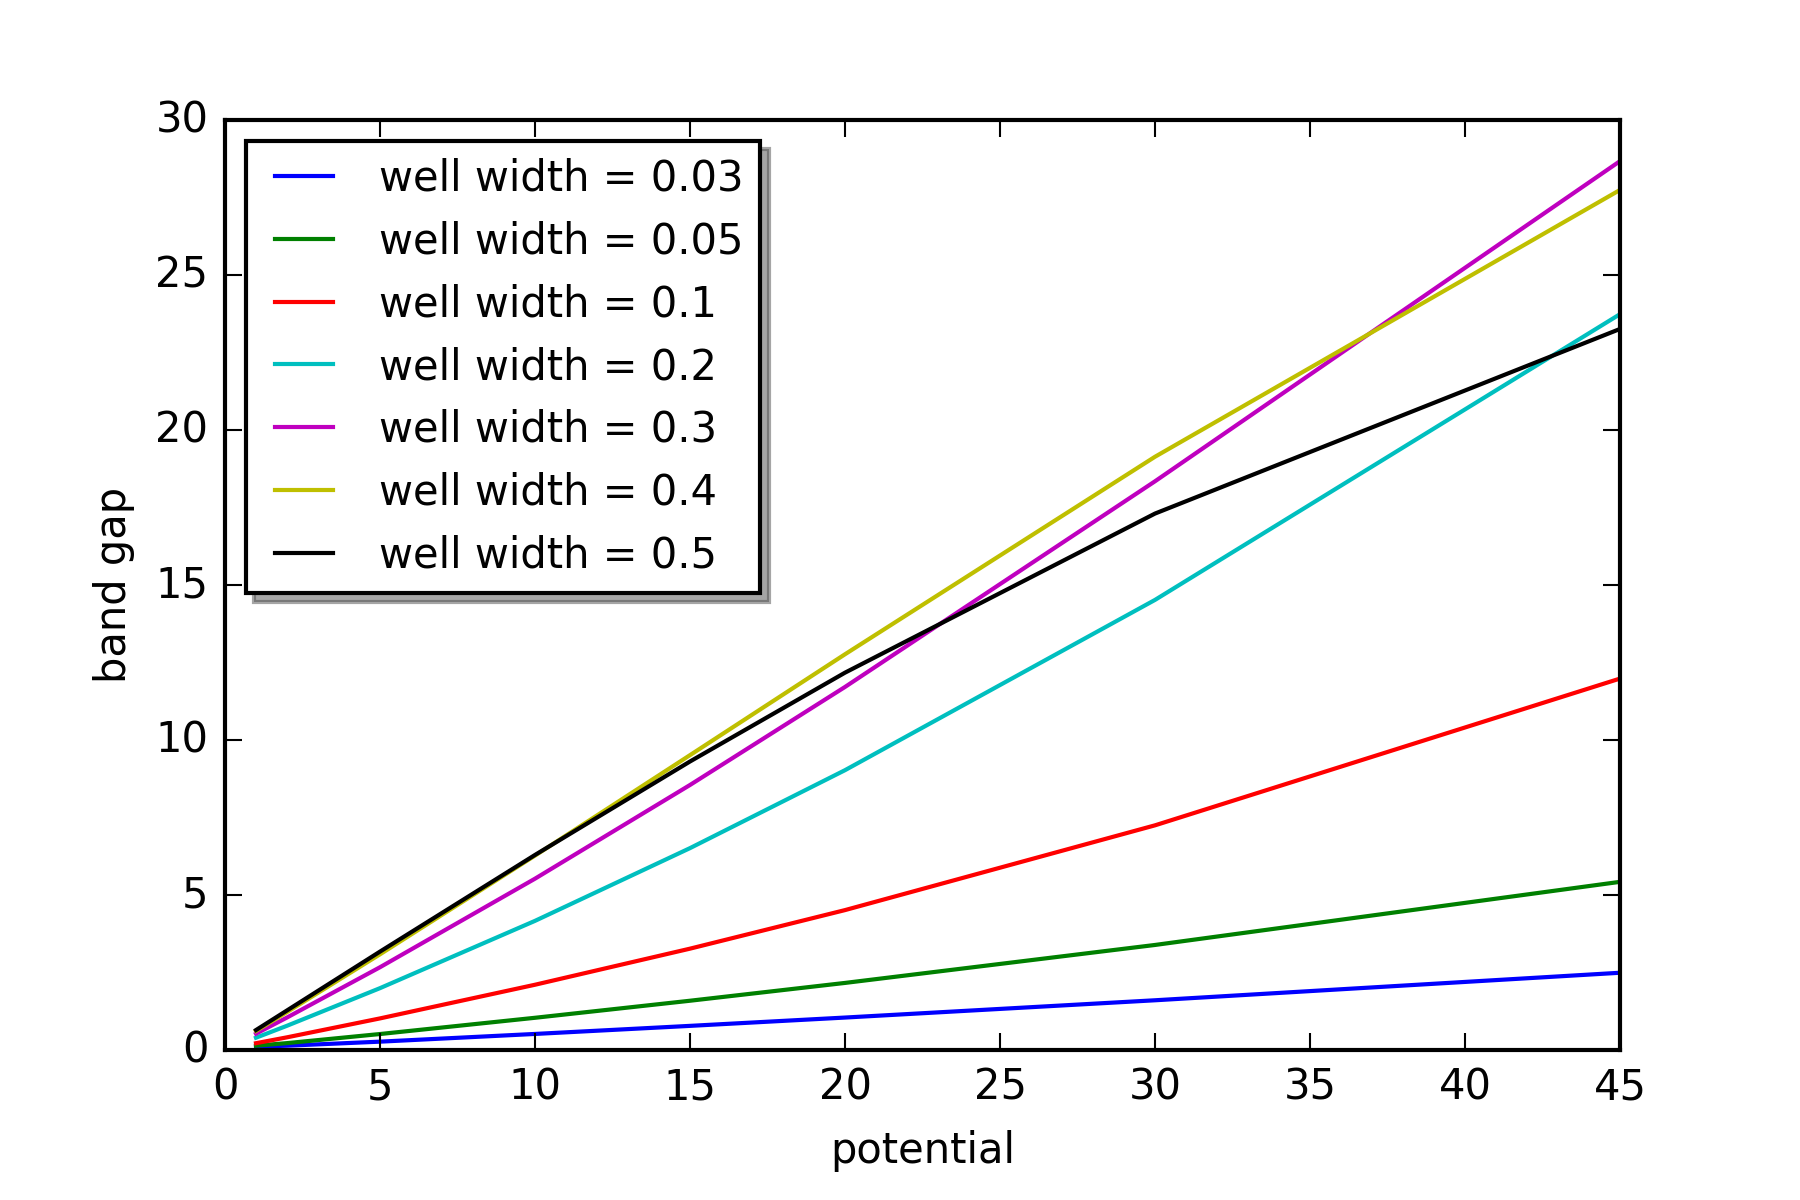
\includegraphics[scale=.8]{Bandgap/30_change_Potentials.png}
\caption{band gap against potential heights at fixed well widths}
\label{fig: band gap against potential }
\end{figure}

We investigate the behavior of band gap when fixing the potential height and varying the well width. 

\begin{figure}[h]
\centering
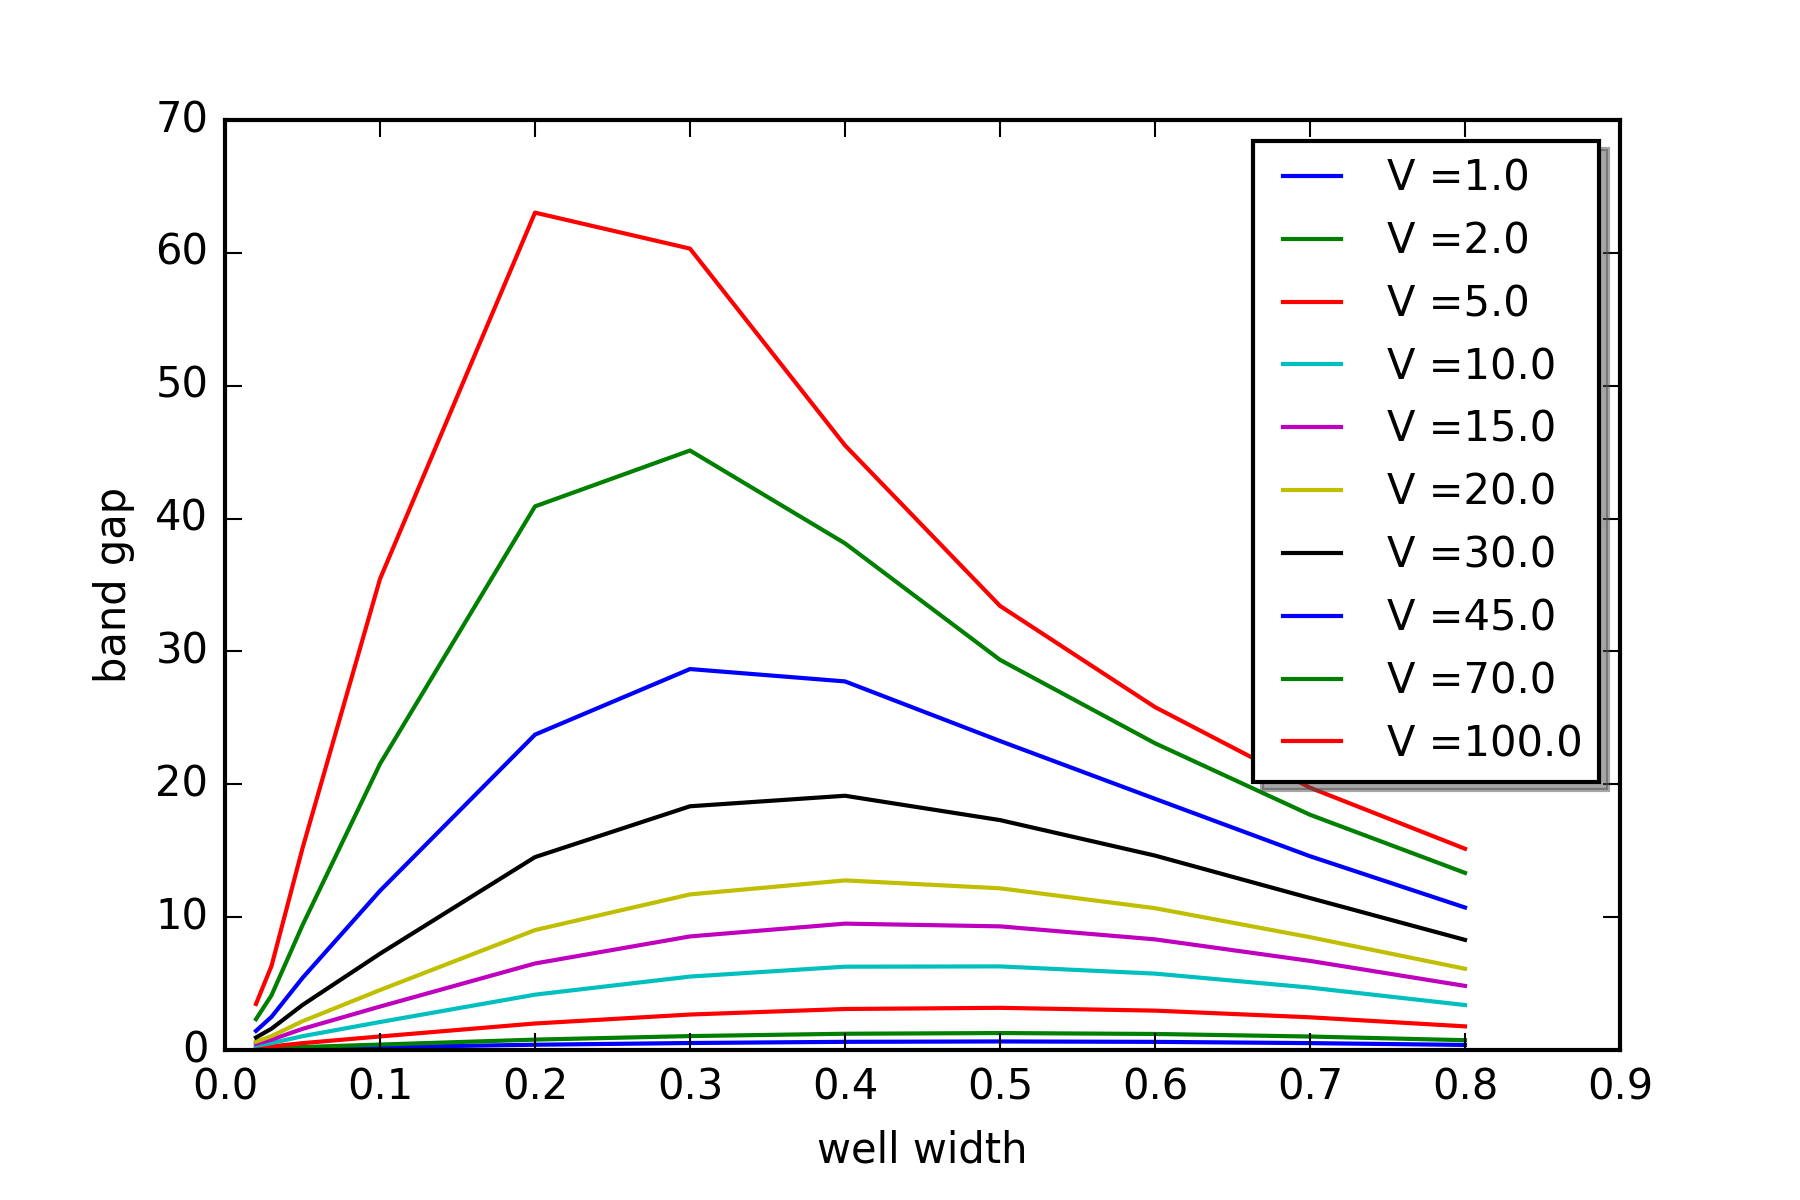
\includegraphics[scale=.8]{Bandgap/complete_change_well_width.png}
\caption{band gap against well width at fixed potentials}
\label{fig:band gap against well width fixed potential}
\end{figure}
\newpage 
Finally, we plot the graph of behavior of band gap when fixing the area of the potential and varying the well width.

\begin{figure}[h]
\centering
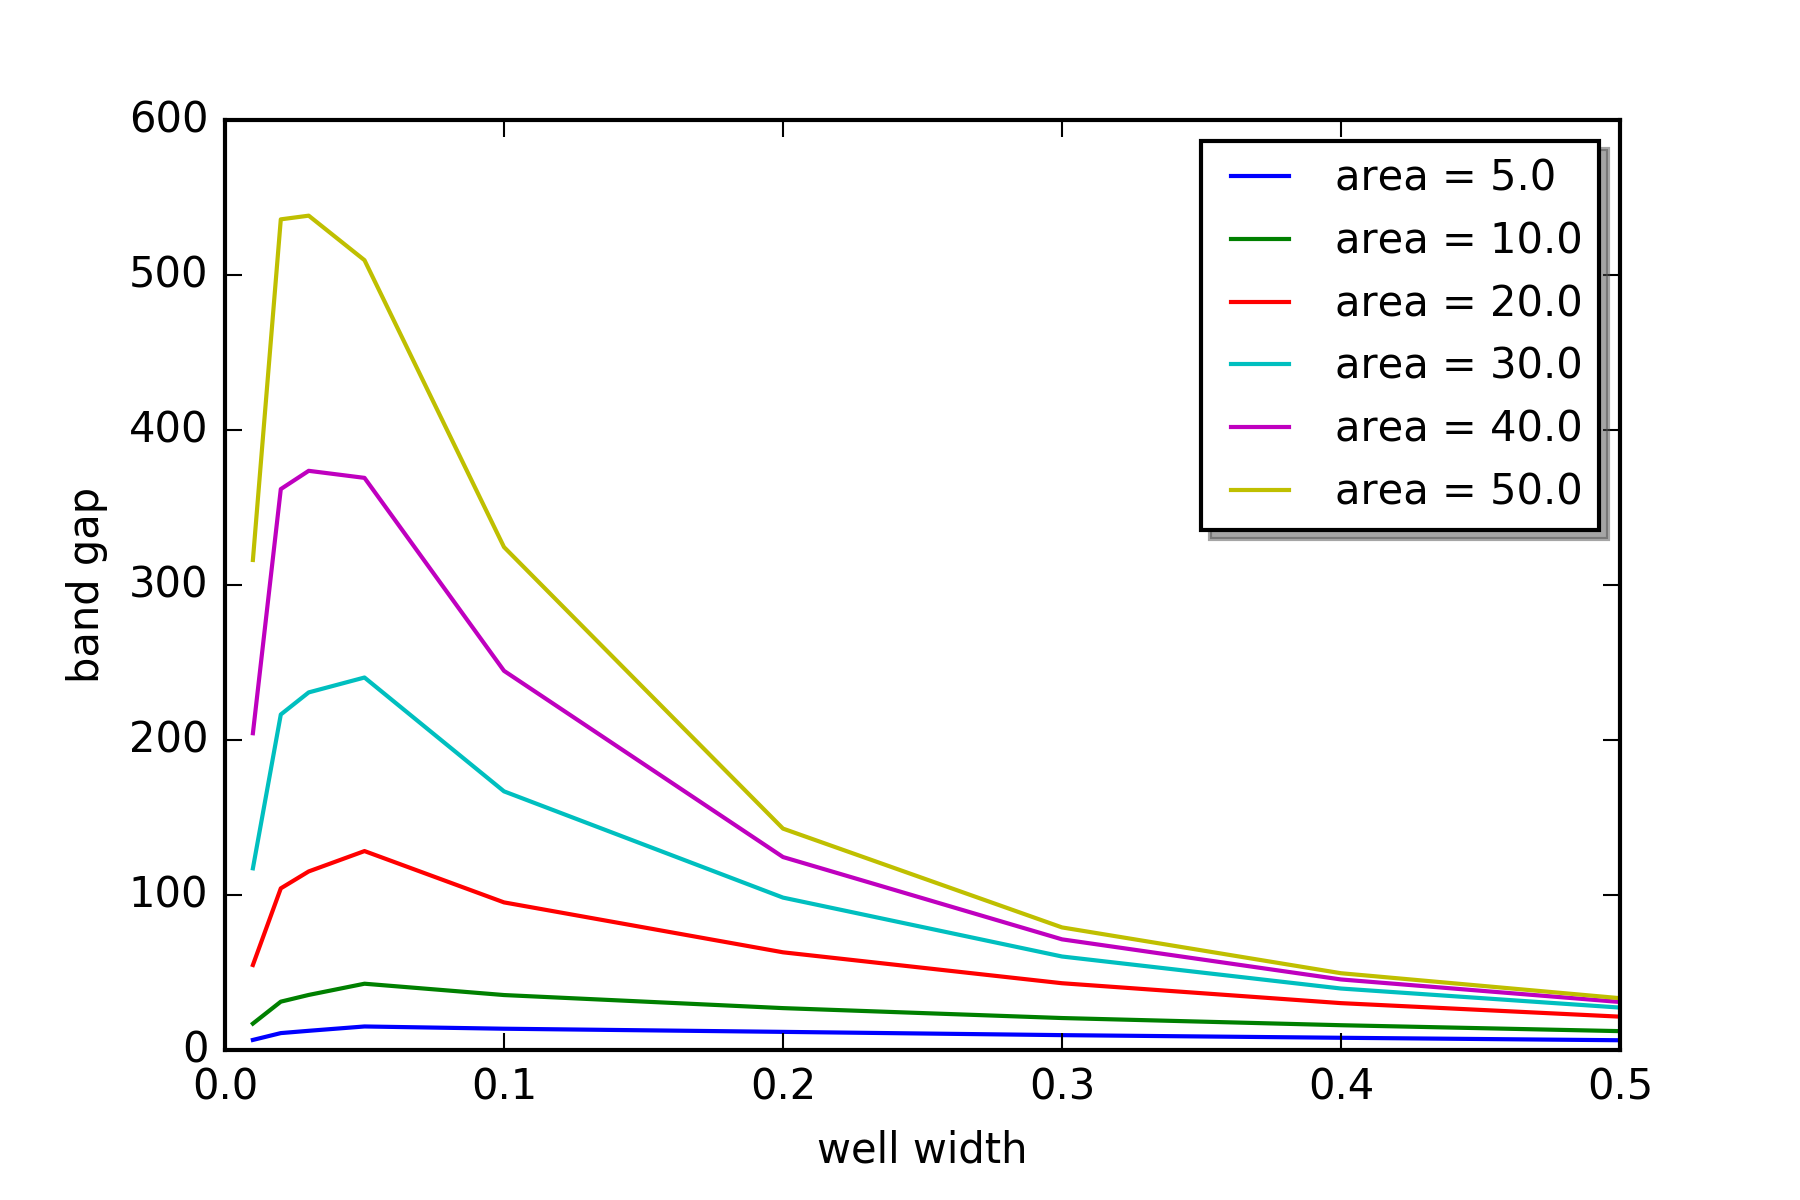
\includegraphics[scale=.8]{Bandgap/change_area5_to_50.png}
\caption{band gap against well width with potential area fixed}
\label{fig:bang gap against well width fixed area}
\end{figure}



\newpage
\section{Localization of eigenstates of Random Kronig Penney Model with zero boundary condition}\label{sec: localization}
In this section, the following figures are for the model we introduced in Chapter \ref{Ch:Background} Section \ref{model:model1}, in which the potential at the boundaries are assumed to be positive infinity, in other words, the wave function at the boundaries is zero.

\subsection{Randomness in atomic spacing}\label{subsec:Randomness in atomic spacing}
The following graphs are the probability density function for both ordered and disordered system under different conditions. The model uses a chain of 31 atoms. The well width is set to be 0.5 for all cases since we are only investigating effect of random spacing between atoms. 

For the ordered system, atoms are equally spaced with 1.0 unit distance.
For the disordered system, the atom spacings are generated from two values$\{p_1,p_2\}$, each with probability 0.5. Then we determine the atom coordinates according to the generated spacings. 

The following are figures for eigenstates of the disordered system when $V_0l$ is equal to 1.
The eigenvalues labeled on each figure are that of an ordered system. 


\begin{figure}[!htbh]
\centering
\begin{minipage}{.45\textwidth}
  \centering
  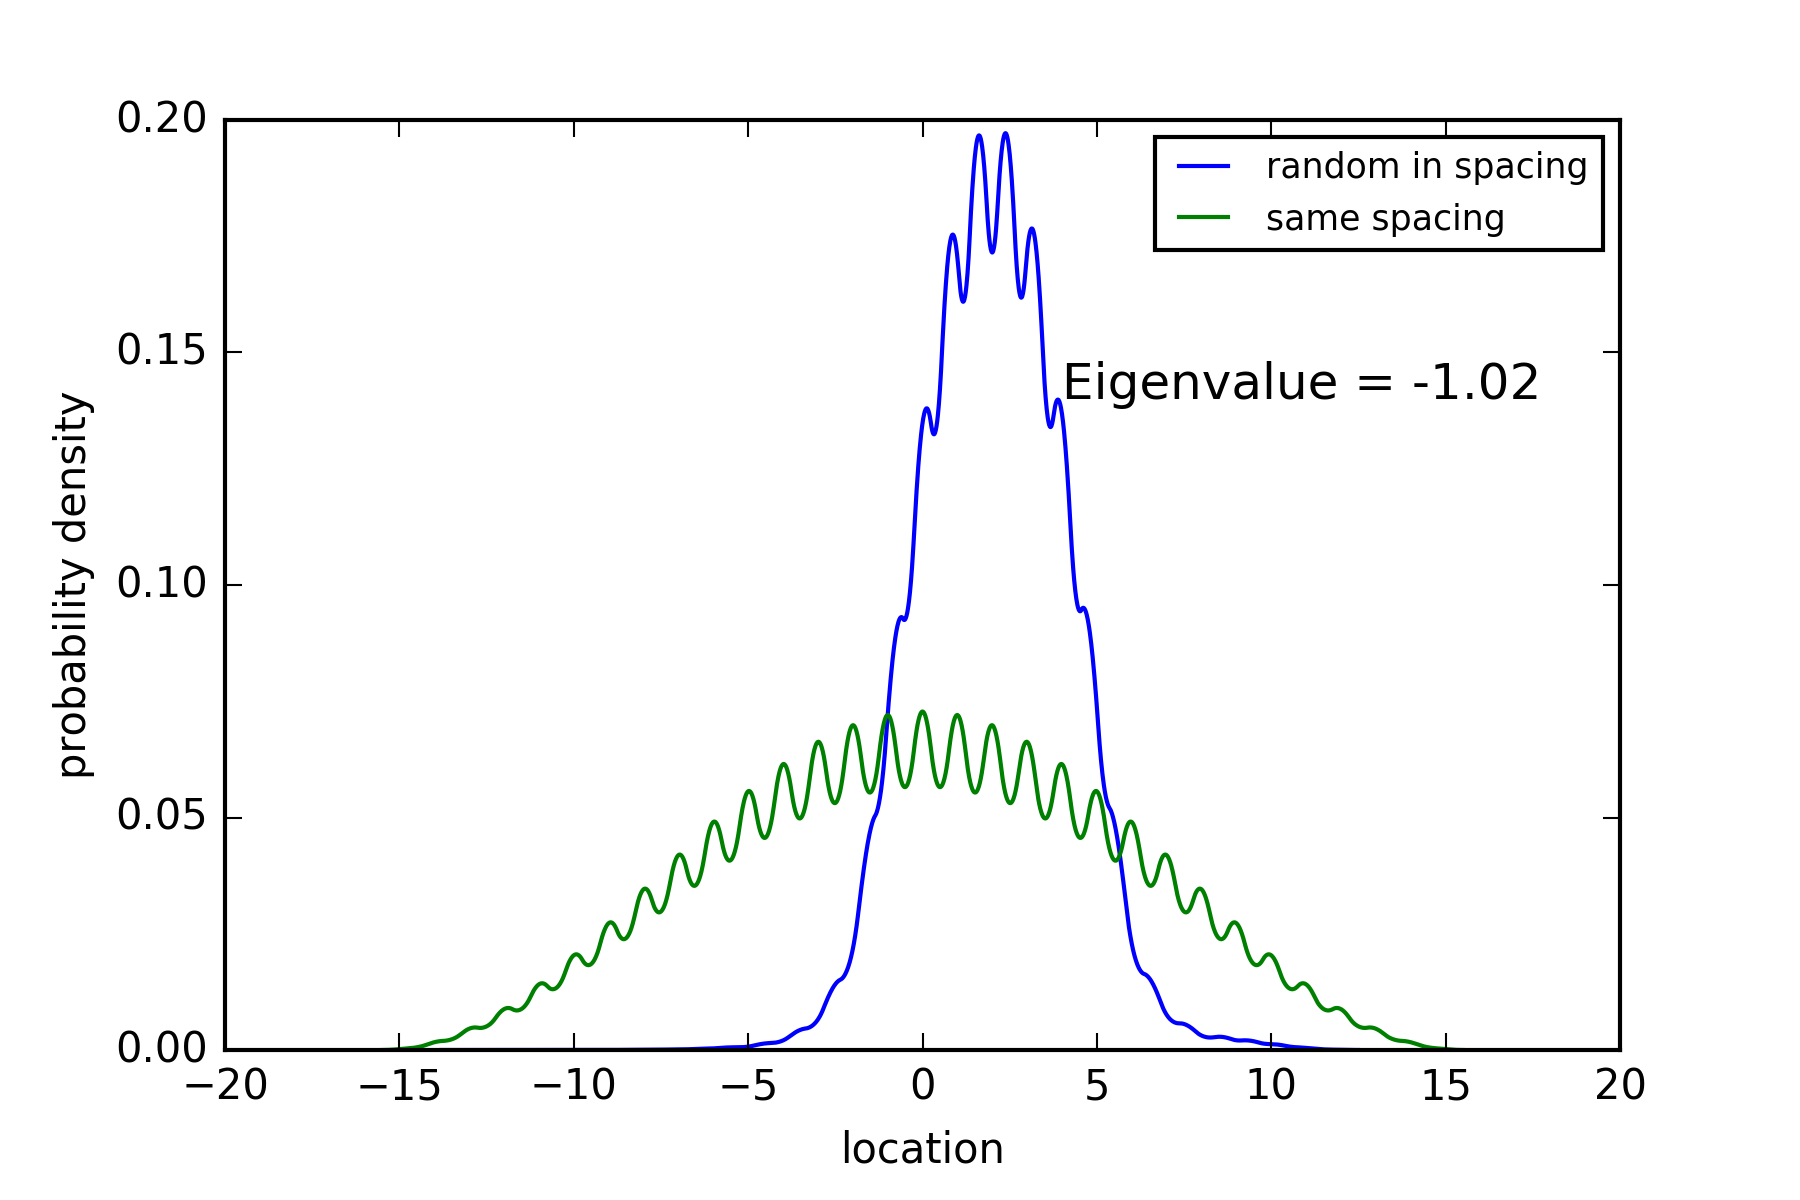
\includegraphics[width=1.1\linewidth]{Graphics/1_0_1th_Lowest_Rand0_8.png}
  \captionof{figure}{Lowest eigenvalue, $V_0l=1$, $\{p_1,p_2\}=\{0.8,1.0\}$}
  \label{fig:Area1_1thlowestRand0.8}
\end{minipage}\qquad
\begin{minipage}{.45\textwidth}
  \centering
  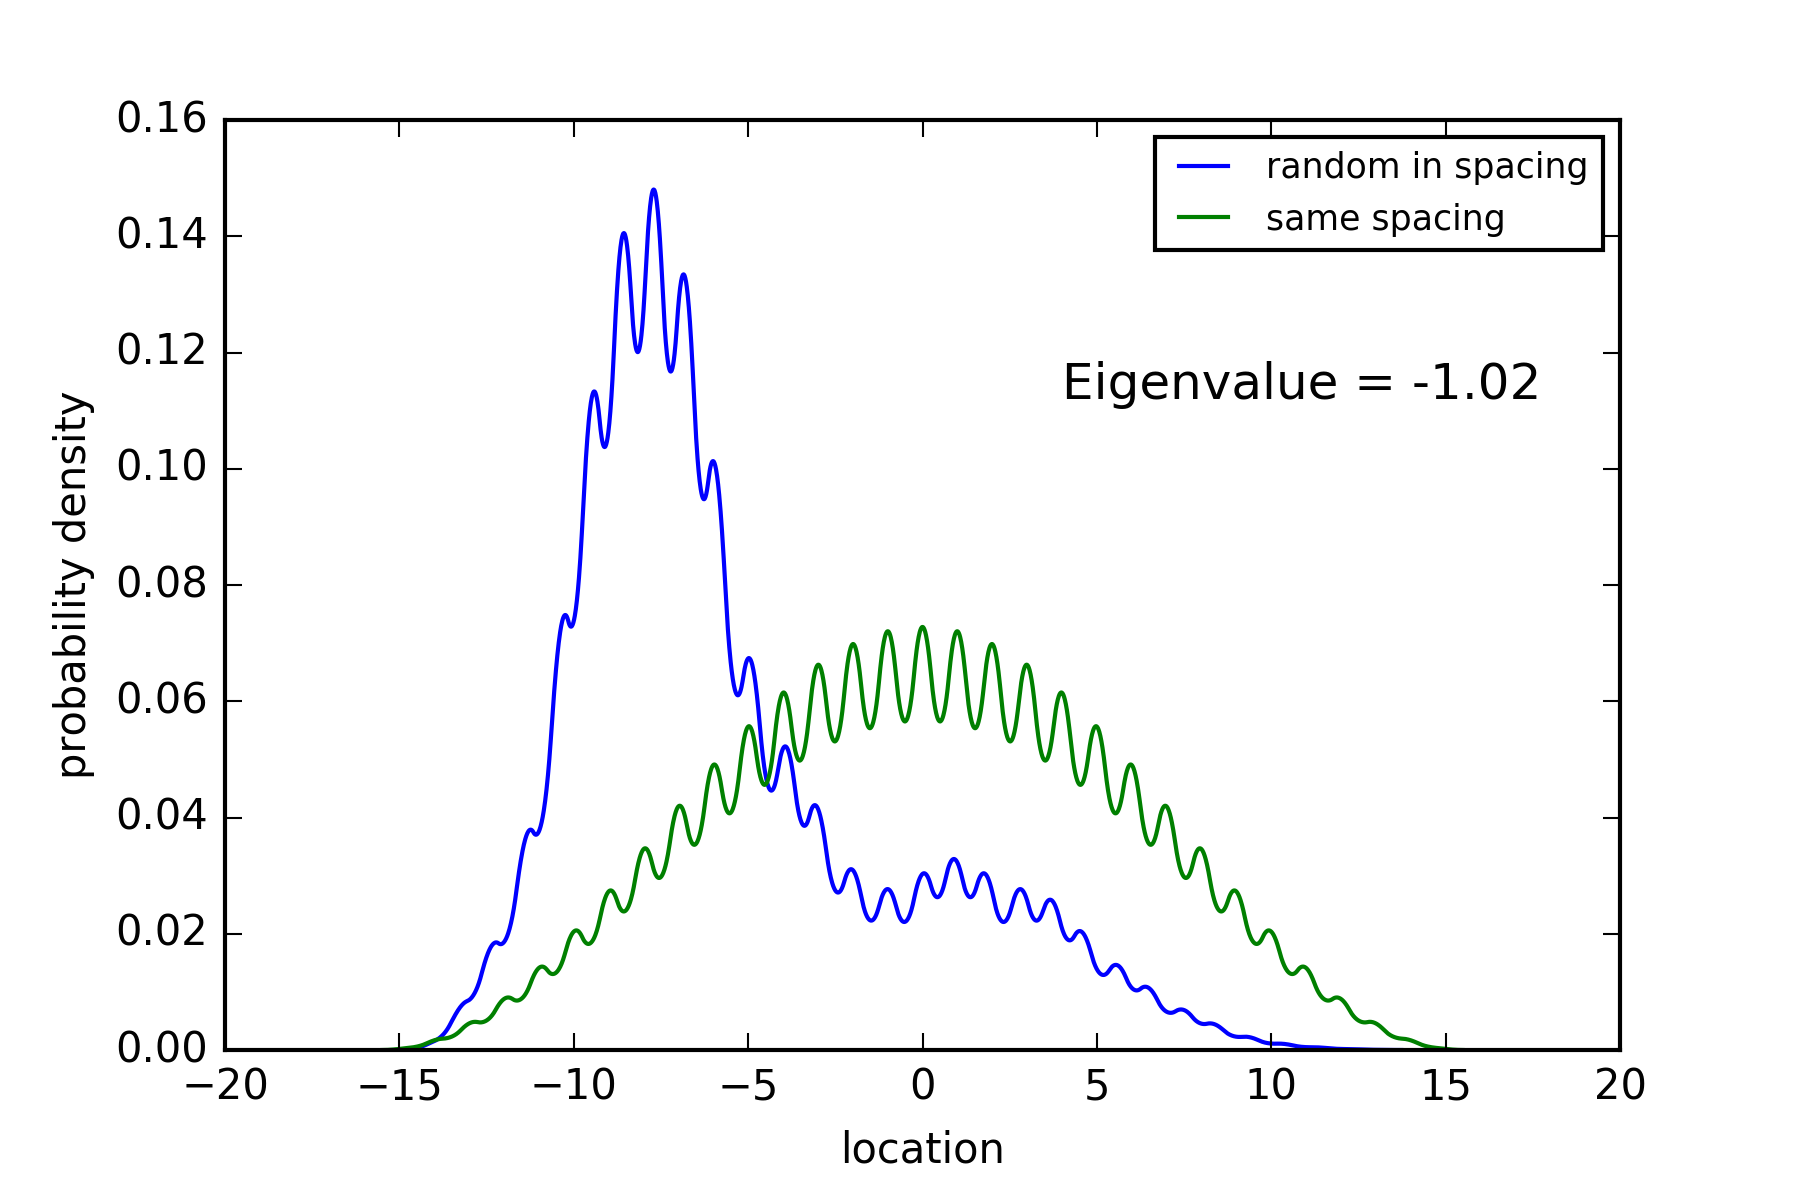
\includegraphics[width=1.1\linewidth]{Graphics/1_0_1th_Lowest_Rand0_9.png}
  \captionof{figure}{Lowest eigenvalue, $V_0l=1$, $\{p_1,p_2\}=\{0.9,1.0\}$}
  \label{fig:Area1_1thlowestRand0.9}
\end{minipage}
\end{figure}

\begin{figure}[!htbh]
\centering
\begin{minipage}{.45\textwidth}
  \centering
  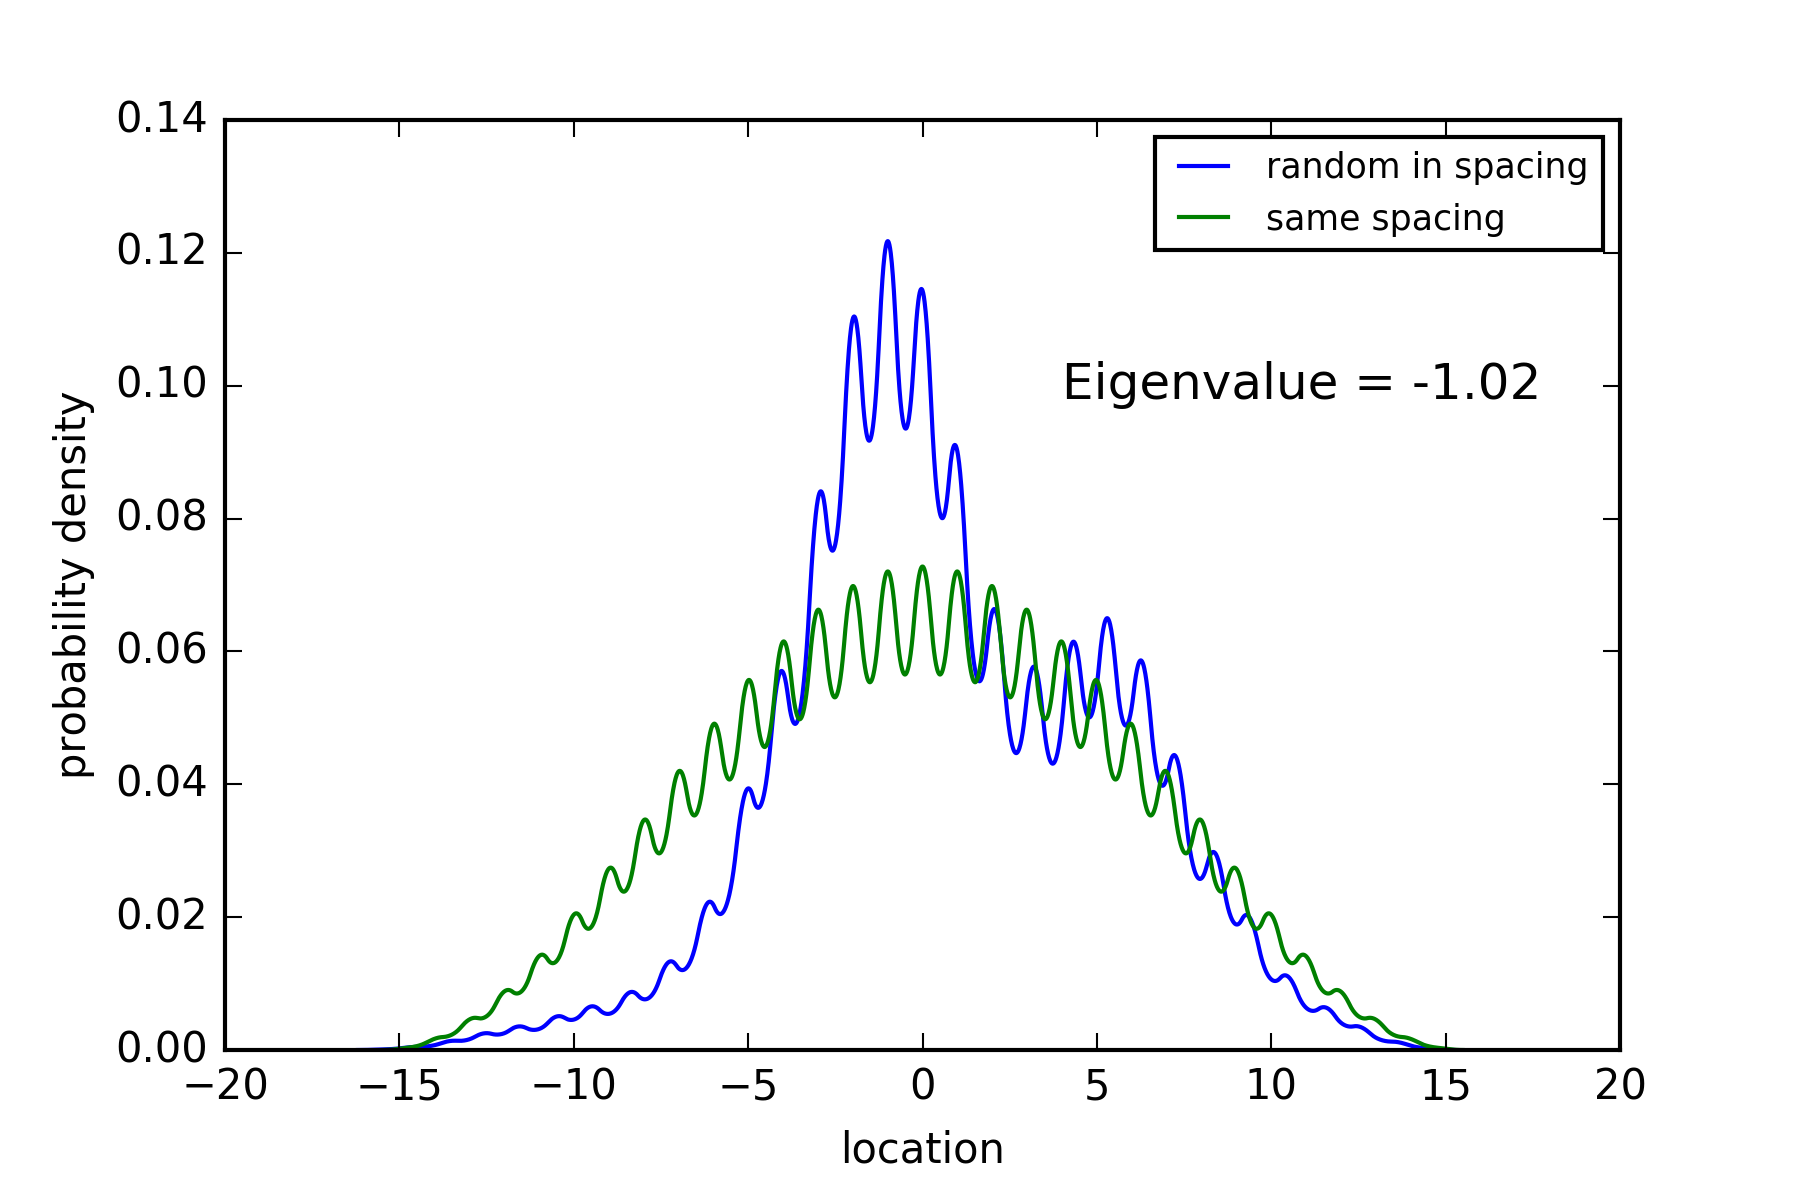
\includegraphics[width=1.1\linewidth]{Graphics/1_0_1th_Lowest_Rand1_1.png}
  \captionof{figure}{Lowest eigenvalue, $V_0l=1$, $\{p_1,p_2\}=\{1.1,1.0\}$}
  \label{fig:Area1_1thlowestRand1.1}
\end{minipage}\qquad
\begin{minipage}{.45\textwidth}
  \centering
  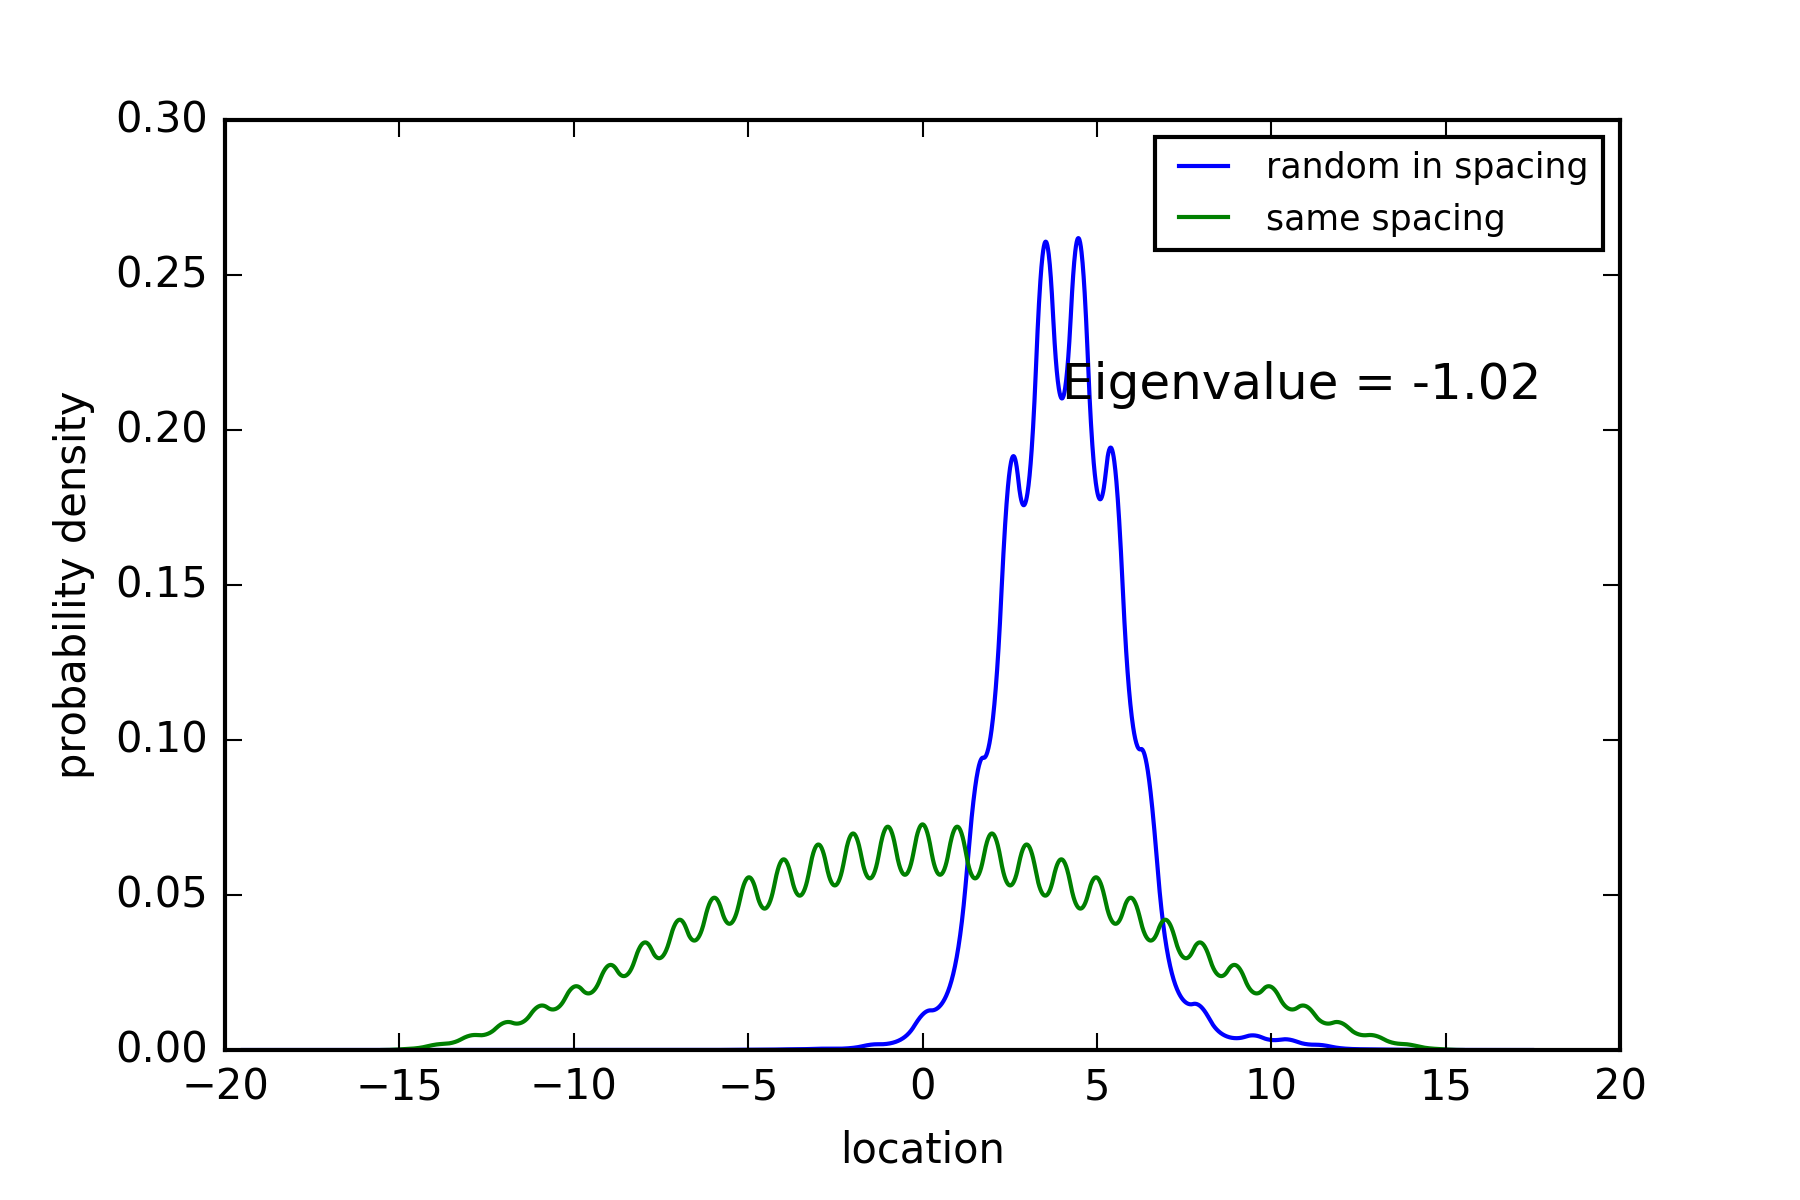
\includegraphics[width=1.1\linewidth]{Graphics/1_0_1th_Lowest_Rand1_5.png}
  \captionof{figure}{Lowest eigenvalue, $V_0l=1$, $\{p_1,p_2\}=\{1.5,1.0\}$}
  \label{fig:Area1_1thlowestRand1.5}
\end{minipage}
\end{figure}

\newpage
The following are figures for the eigenstate of the disordered system when $V_0l$ is equal to 10.

\begin{figure}[!htbh]
\centering
\begin{minipage}{.45\textwidth}
  \centering
  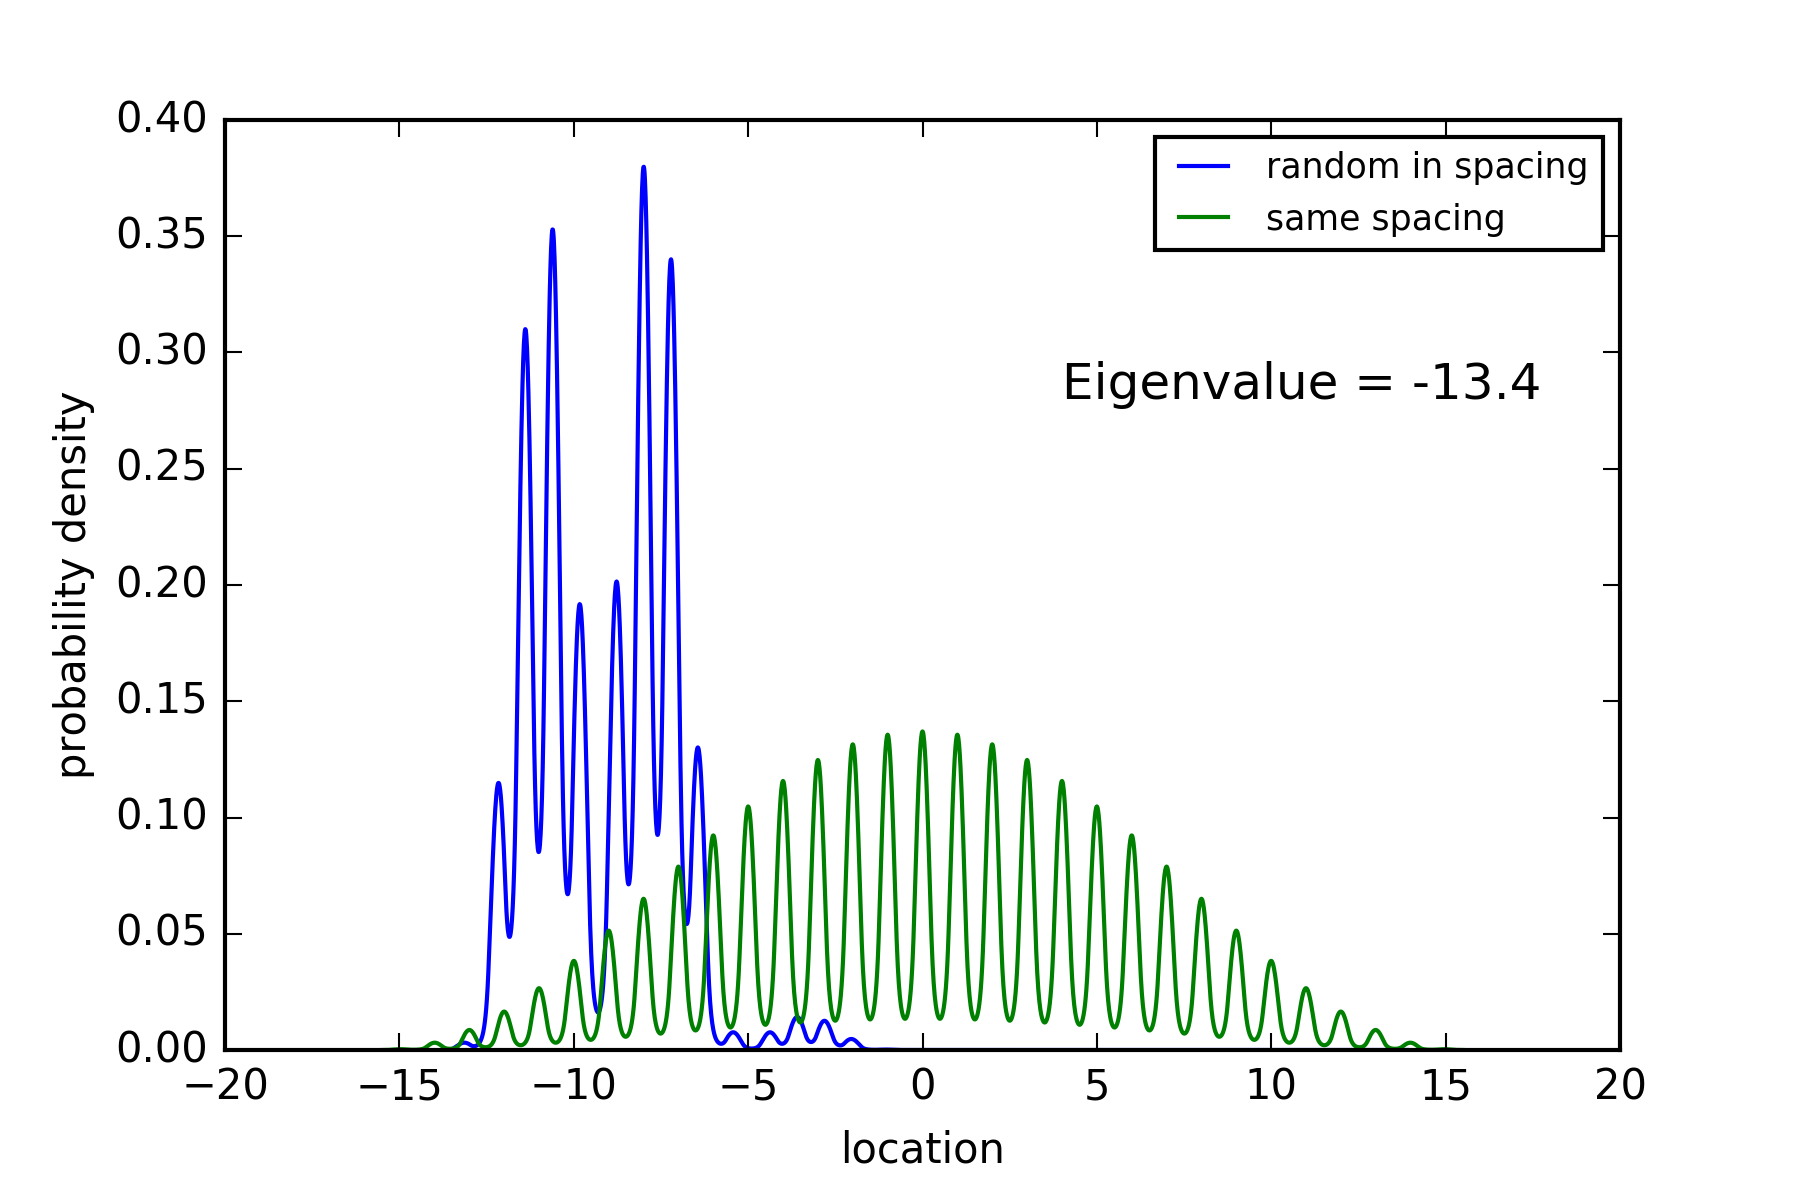
\includegraphics[width=1.1\linewidth]{Graphics/10_0_1th_Lowest_Rand0_8.png}
  \captionof{figure}{Lowest eigenvalue, $V_0l=10.0$ ,$\{p_1,p_2\}=\{0.8,1.0\}$}
  \label{fig:Area10_1thlowestRand0.8}
\end{minipage}\qquad
\begin{minipage}{.45\textwidth}
  \centering
  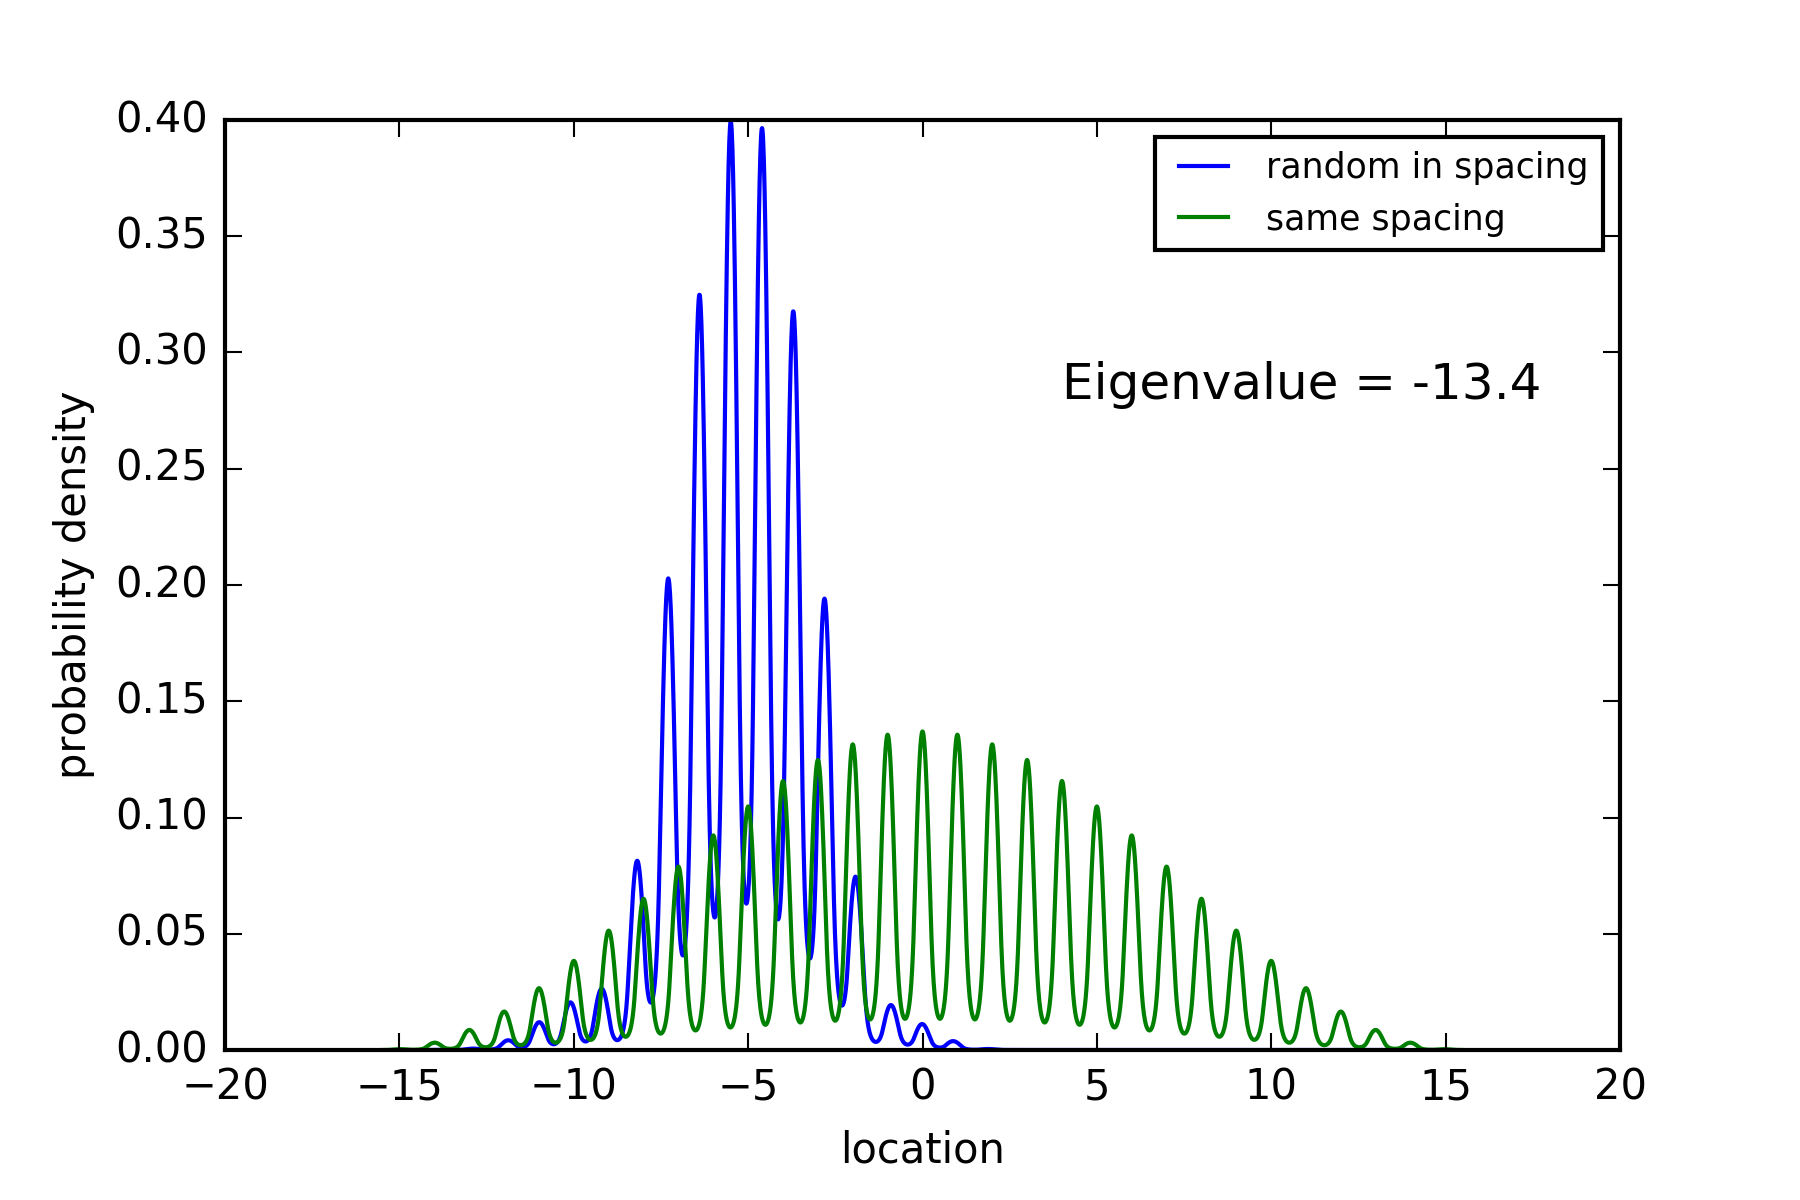
\includegraphics[width=1.1\linewidth]{Graphics/10_0_1th_Lowest_Rand0_9.png}
  \captionof{figure}{Lowest eigenvalue, $V_0l=10.0$, $\{p_1,p_2\}=\{0.9,1.0\}$}
  \label{fig:Area10_1thlowestRand0.9}
\end{minipage}
\end{figure}

\begin{figure}[!htbh]
\centering
\begin{minipage}{.45\textwidth}
  \centering
  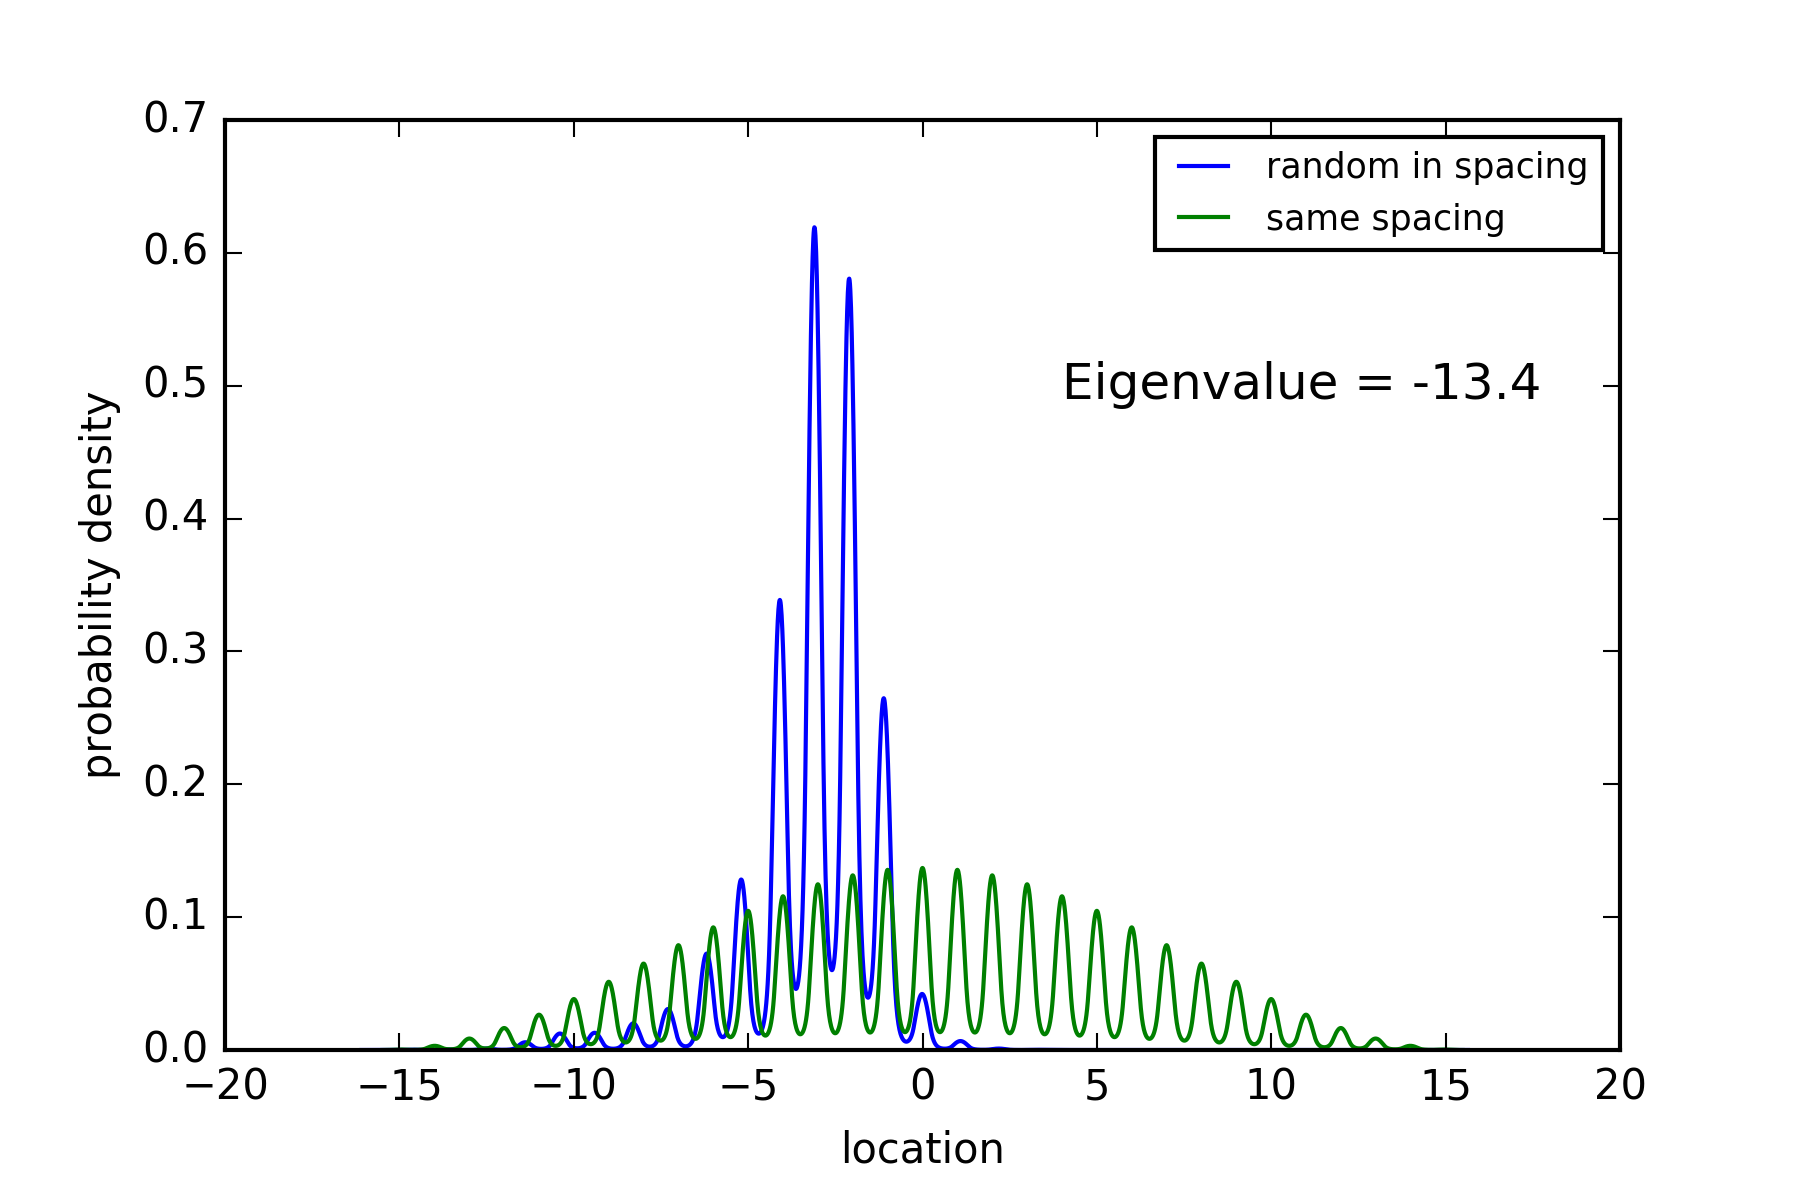
\includegraphics[width=1.1\linewidth]{Graphics/10_0_1th_Lowest_Rand1_1.png}
  \captionof{figure}{Lowest eigenvalue, $V_0l=10.0$, $\{p_1,p_2\}=\{1.1,1.0\}$}
  \label{fig:Area10_1thlowestRand1.1}
\end{minipage}\qquad
\begin{minipage}{.45\textwidth}
  \centering
  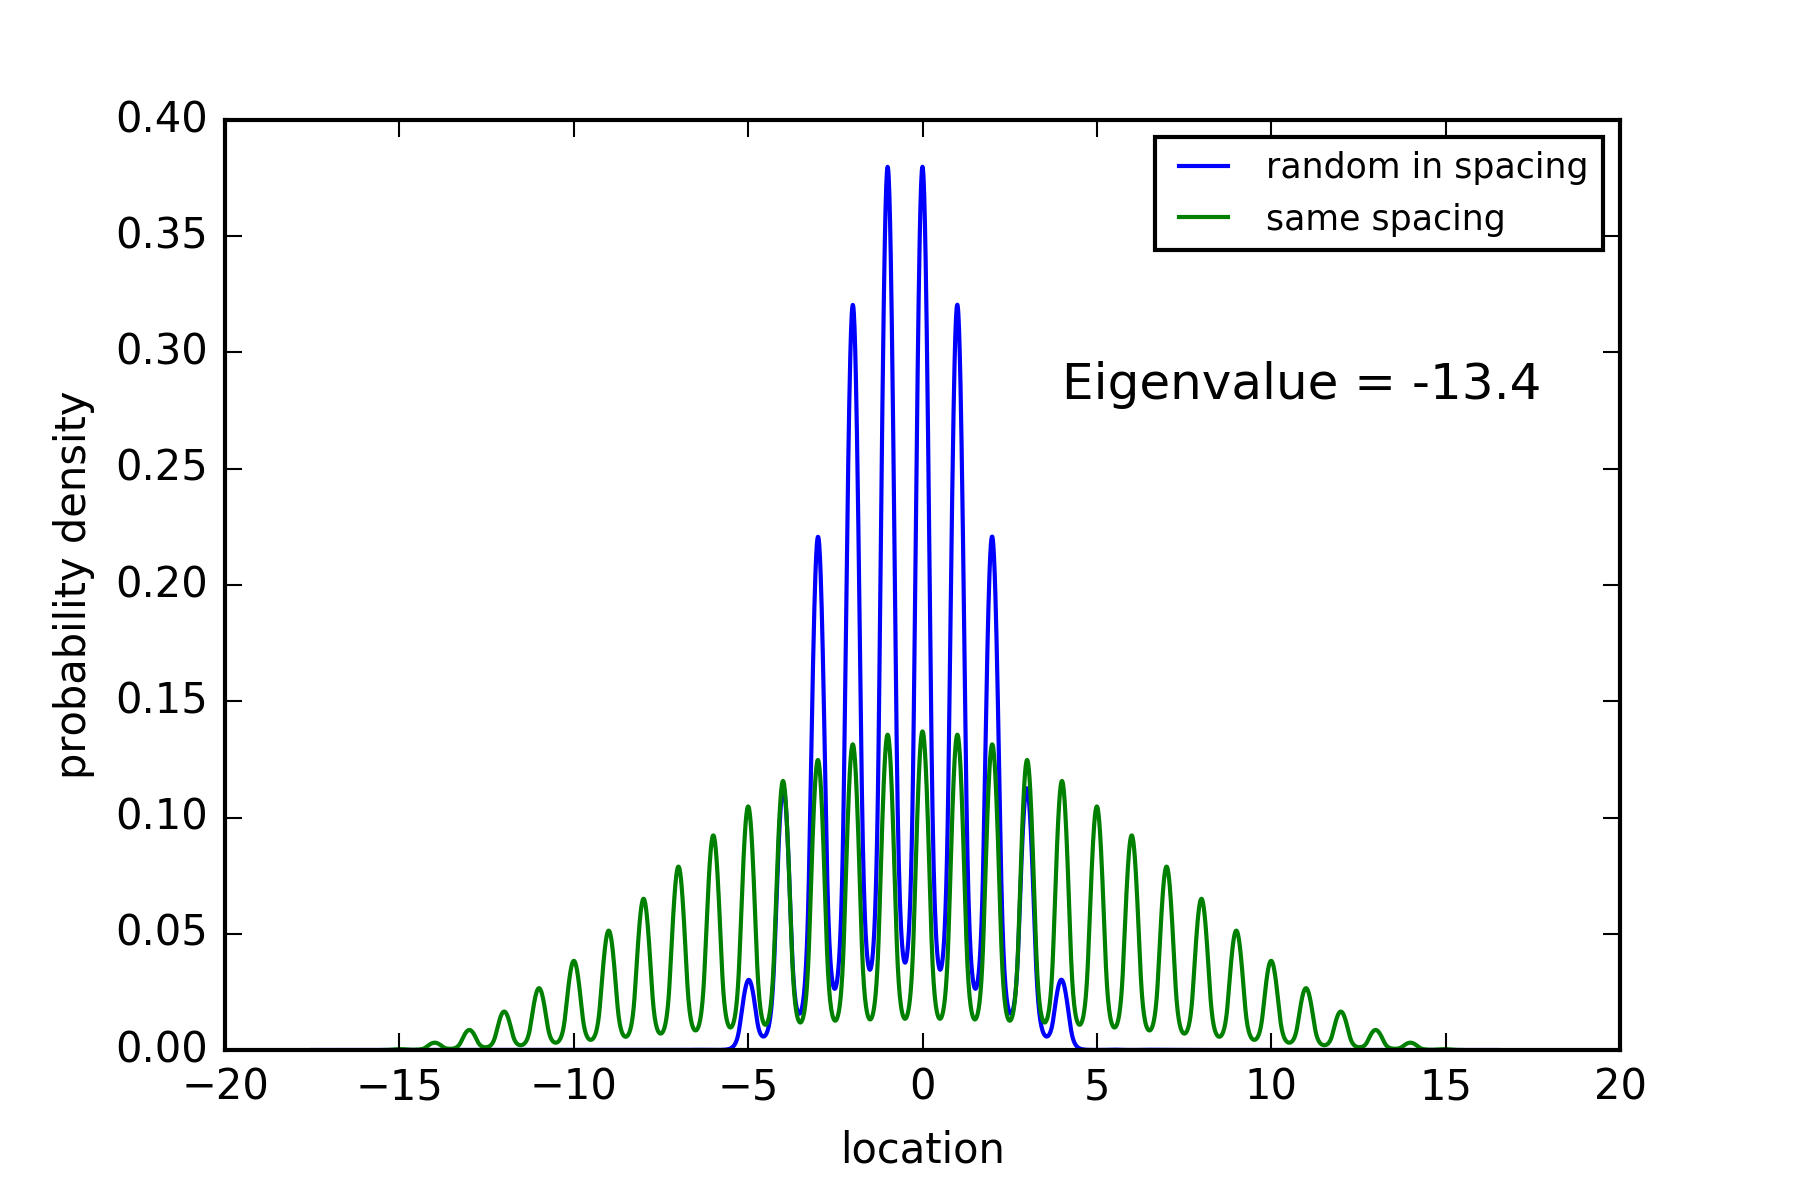
\includegraphics[width=1.1\linewidth]{Graphics/10_0_1th_Lowest_Rand1_5.png}
  \captionof{figure}{Lowest eigenvalue, $V_0l=10.0$, $\{p_1,p_2\}=\{1.5,1.0\}$}
  \label{fig:Area10_1thlowestRand1.5}
\end{minipage}
\end{figure}

% modified Wed 15:15 pm

The following are figures for the eigenstate corresponding to the second lowest eigenenergy. Again, $V_0l$ is equal to 1 for the first 4 figures, and 10 for the other 4 figures. They are in the same order as the eigenstates for the lowest eigenenergy.

%2nd lowest, Vl = 1.0
\begin{figure}[!htbh]
\centering
\begin{minipage}{.45\textwidth}
  \centering
  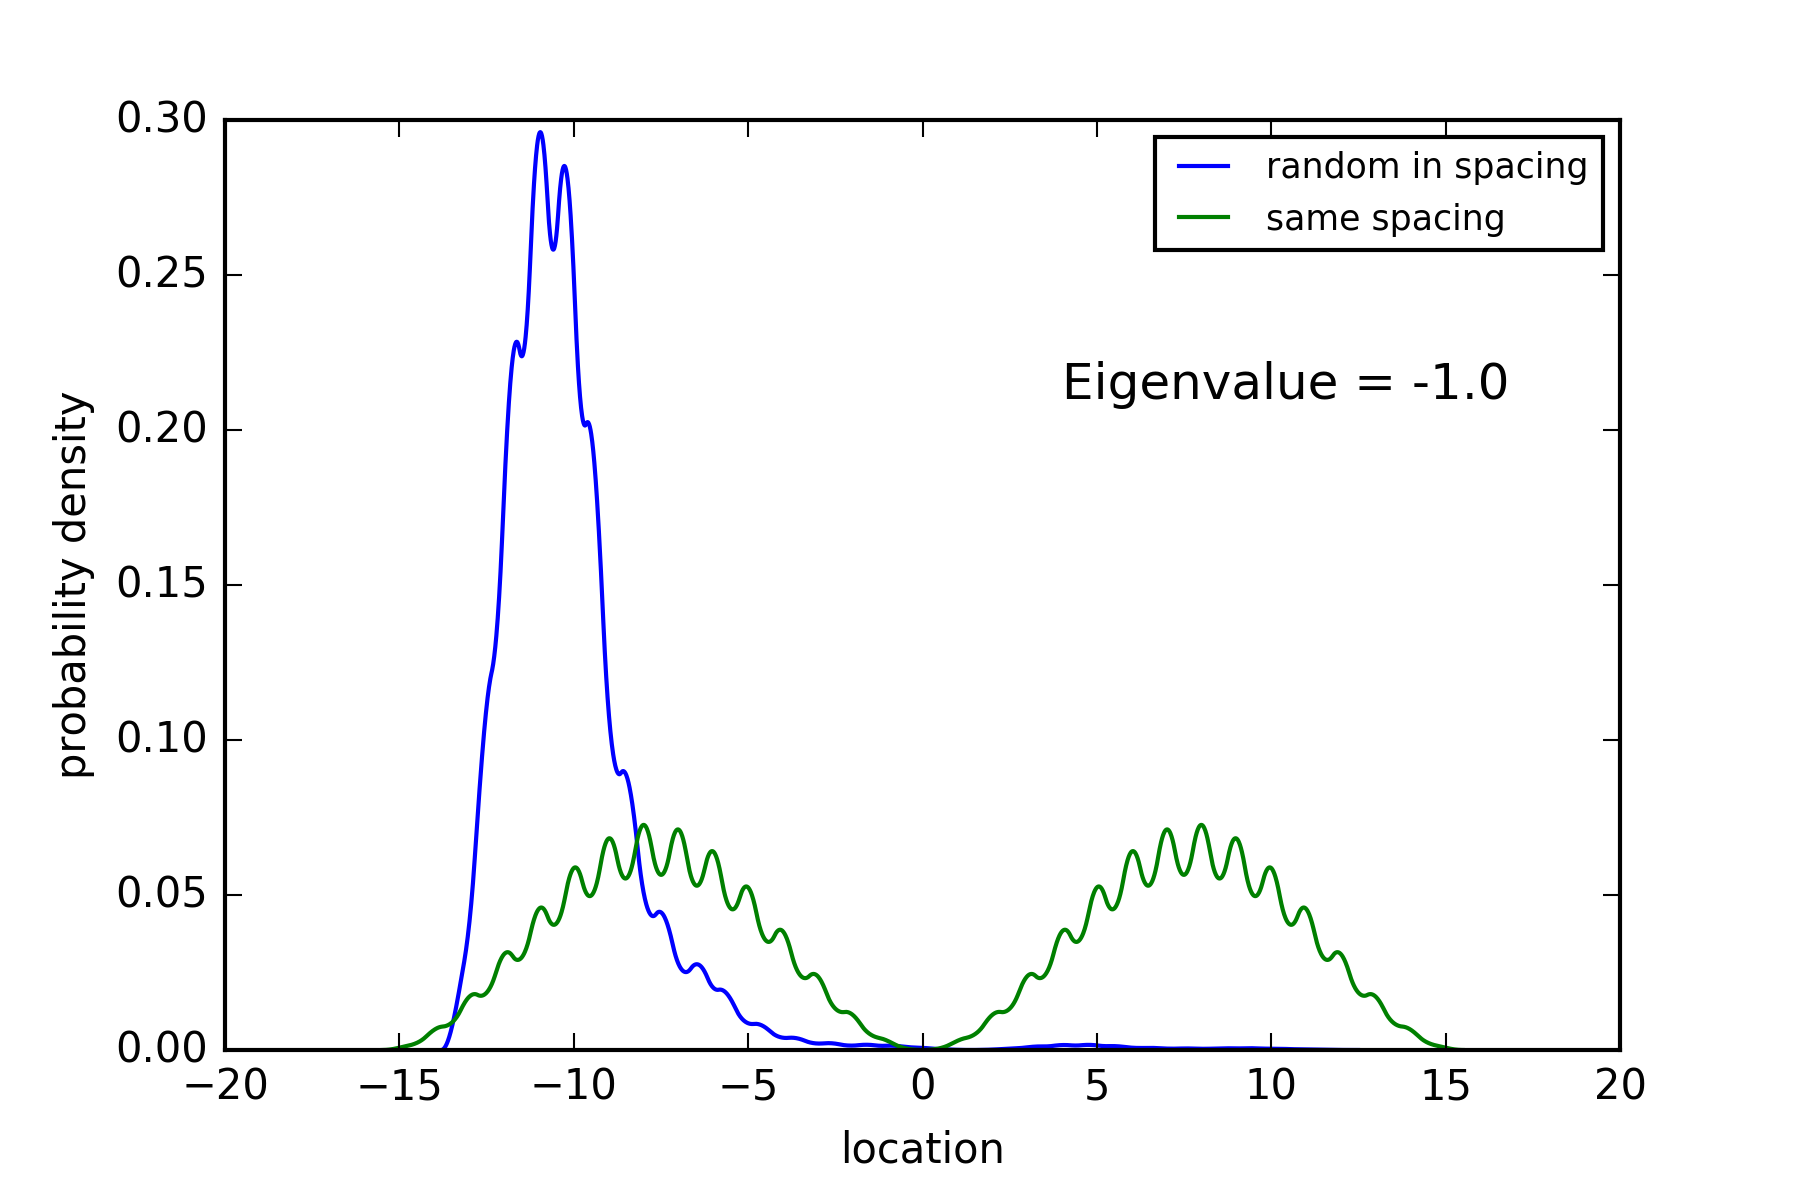
\includegraphics[width=1.1\linewidth]{Graphics/1_0_2th_Lowest_Rand0_8.png}
  \captionof{figure}{2nd Lowest eigenvalue, $V_0l=1.0$, $\{p_1,p_2\}=\{0.8,1.0\}$}
  \label{fig:Area1_2thlowestRand0.8}
\end{minipage}\qquad
\begin{minipage}{.45\textwidth}
  \centering
  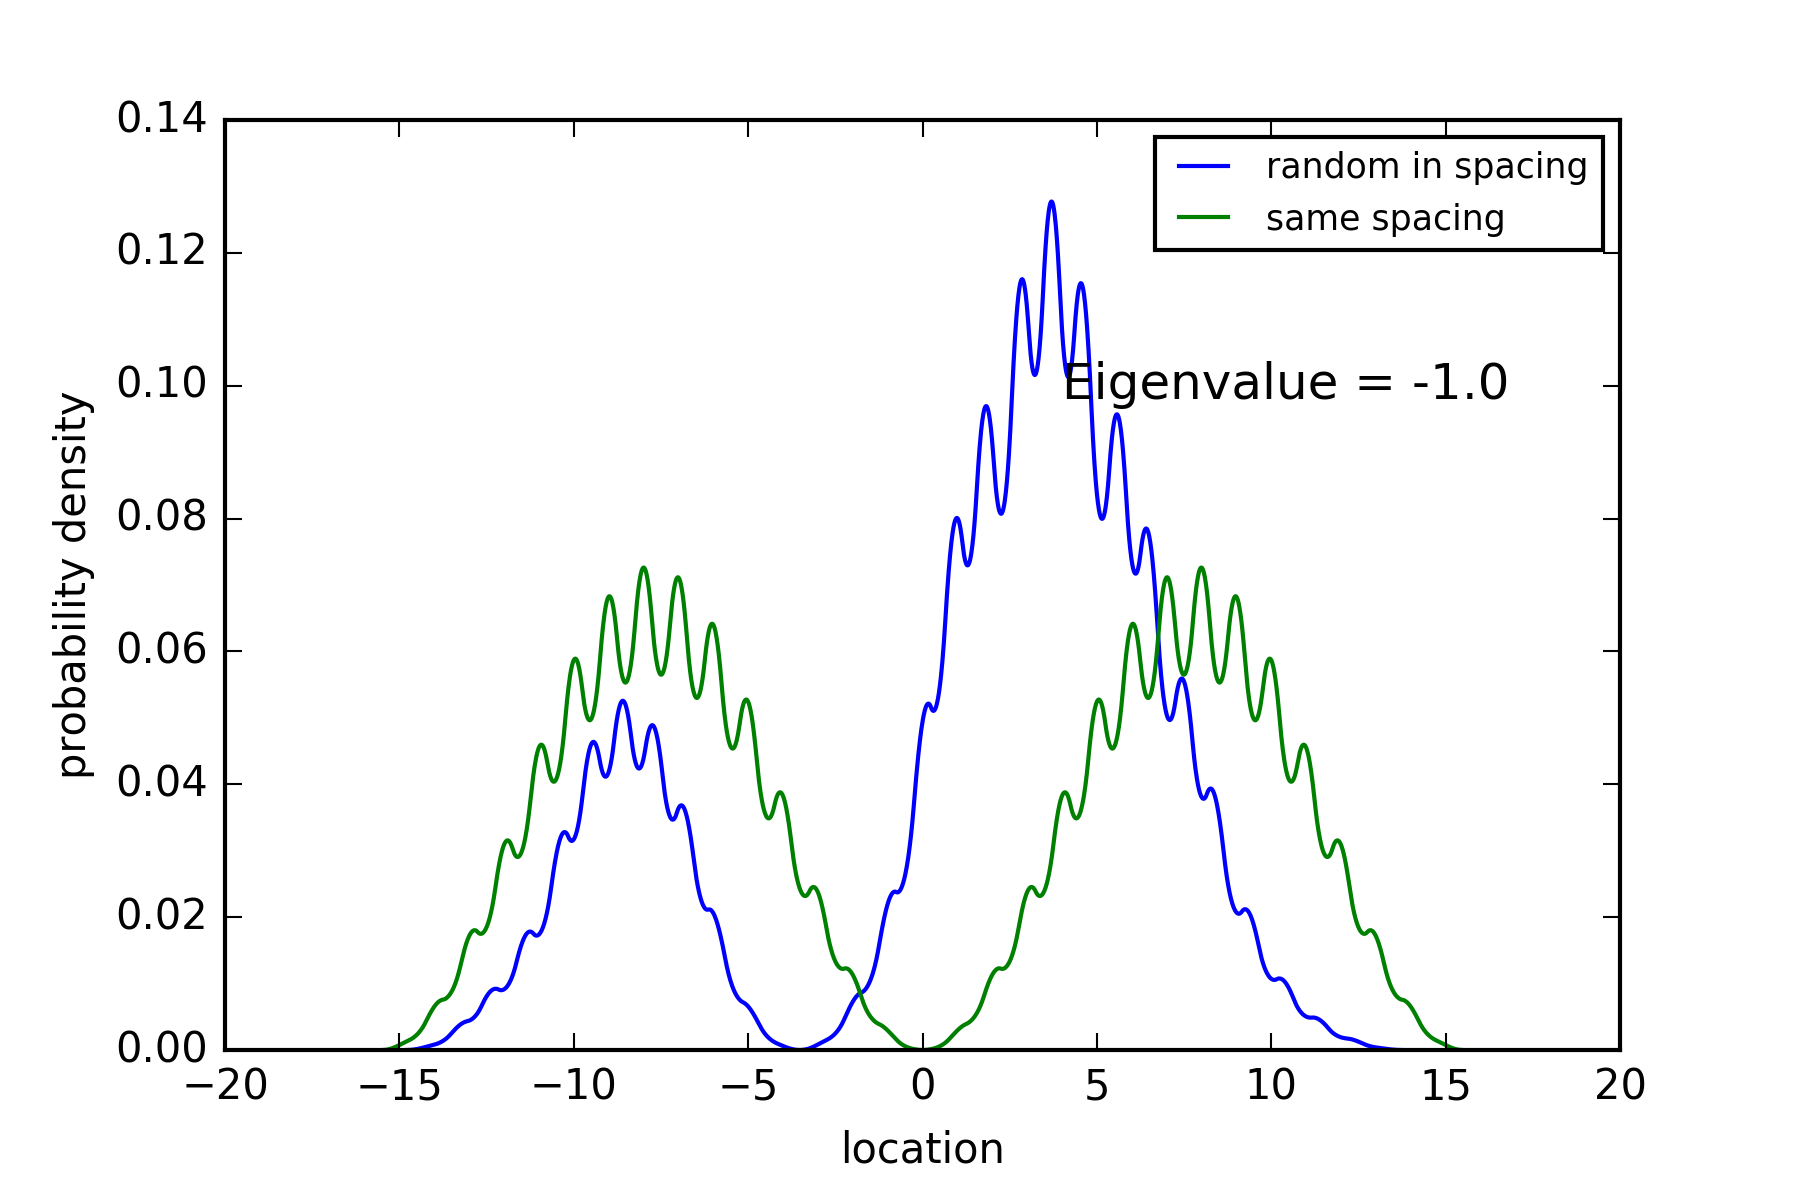
\includegraphics[width=1.1\linewidth]{Graphics/1_0_2th_Lowest_Rand0_9.png}
  \captionof{figure}{2nd Lowest eigenvalue, $V_0l=1.0$, $\{p_1,p_2\}=\{0.9,1.0\}$}
  \label{fig:Area1_2thlowestRand0.9}
\end{minipage}
\end{figure}

\begin{figure}[!htbh]
\centering
\begin{minipage}{.45\textwidth}
  \centering
  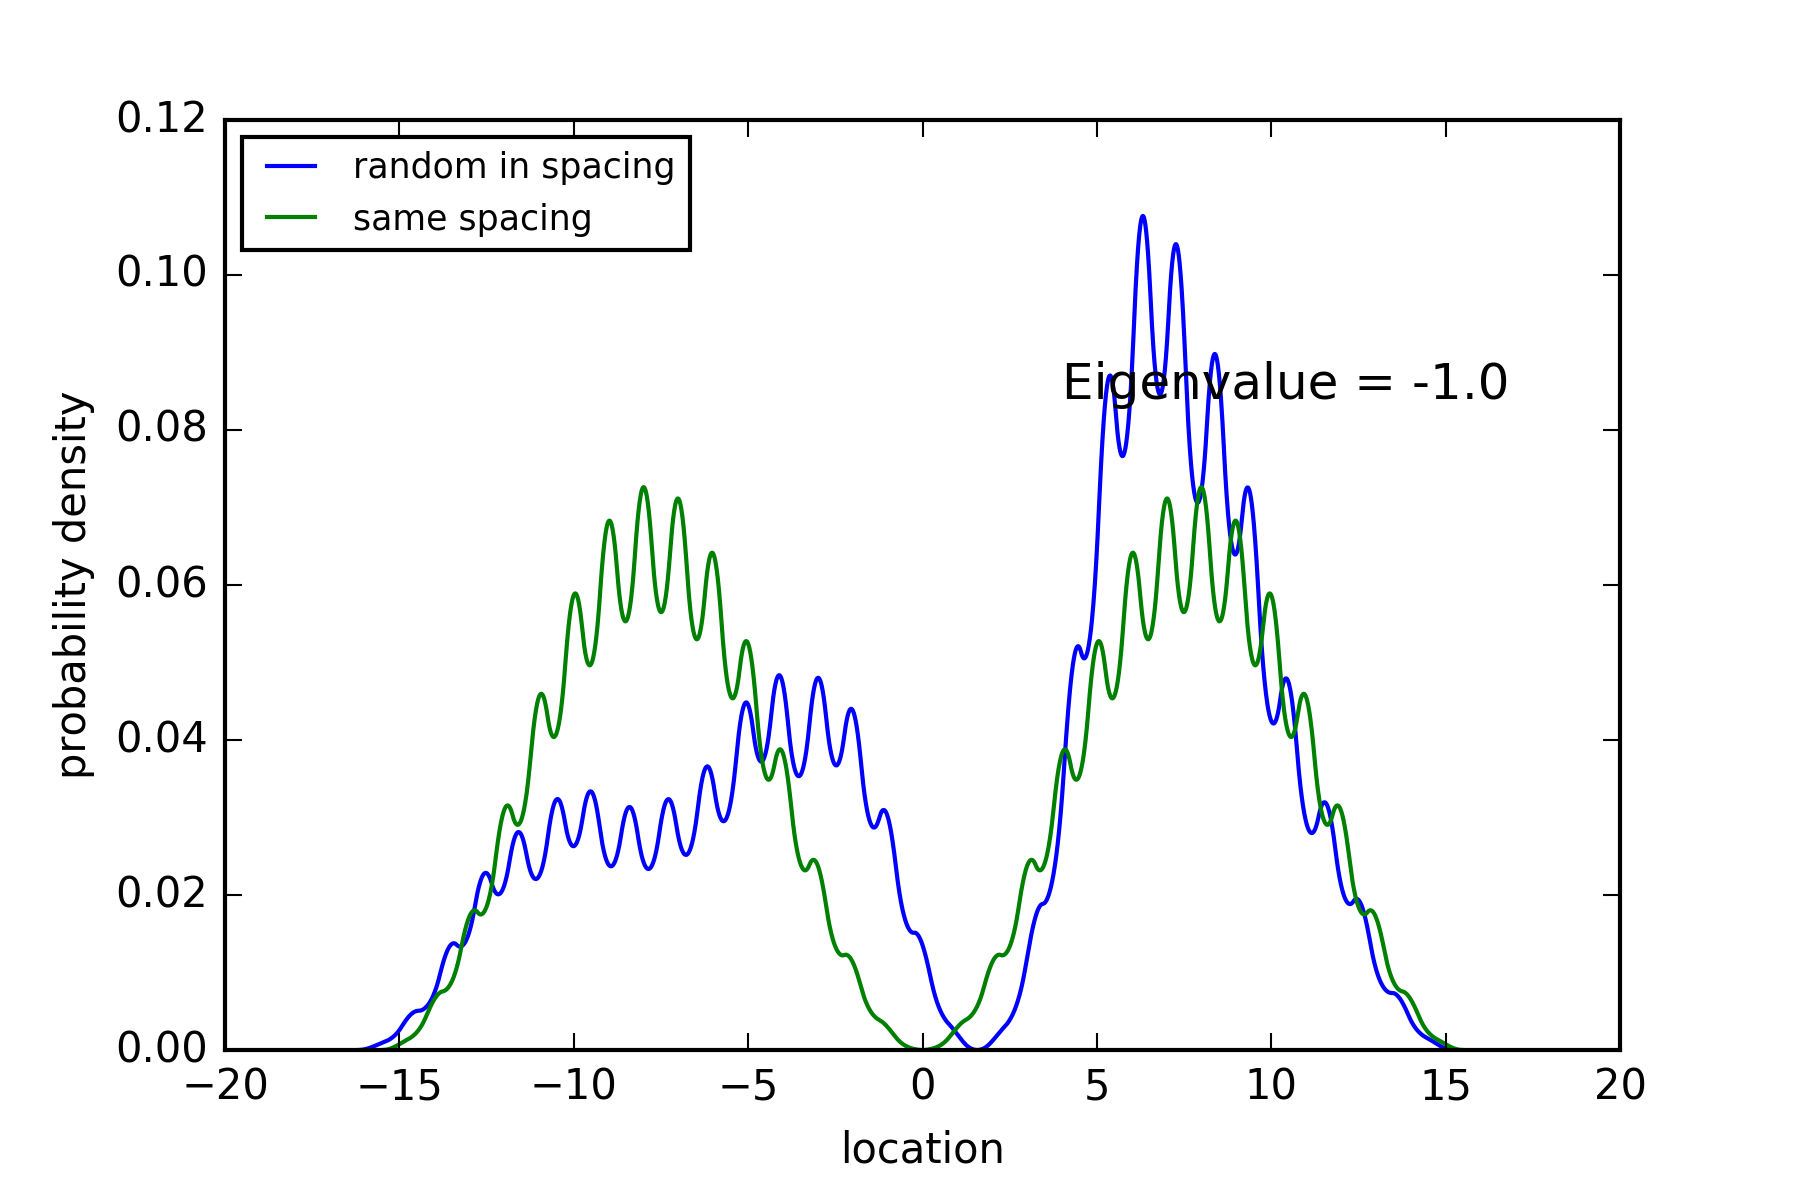
\includegraphics[width=1.1\linewidth]{Graphics/1_0_2th_Lowest_Rand1_1.png}
  \captionof{figure}{2nd Lowest eigenvalue, $V_0l = 1.0$, $\{p_1,p_2\}=\{1.1,1.0\}$}
  \label{fig:Area1_2thlowestRand1.1}
\end{minipage}\qquad
\begin{minipage}{.45\textwidth}
  \centering
  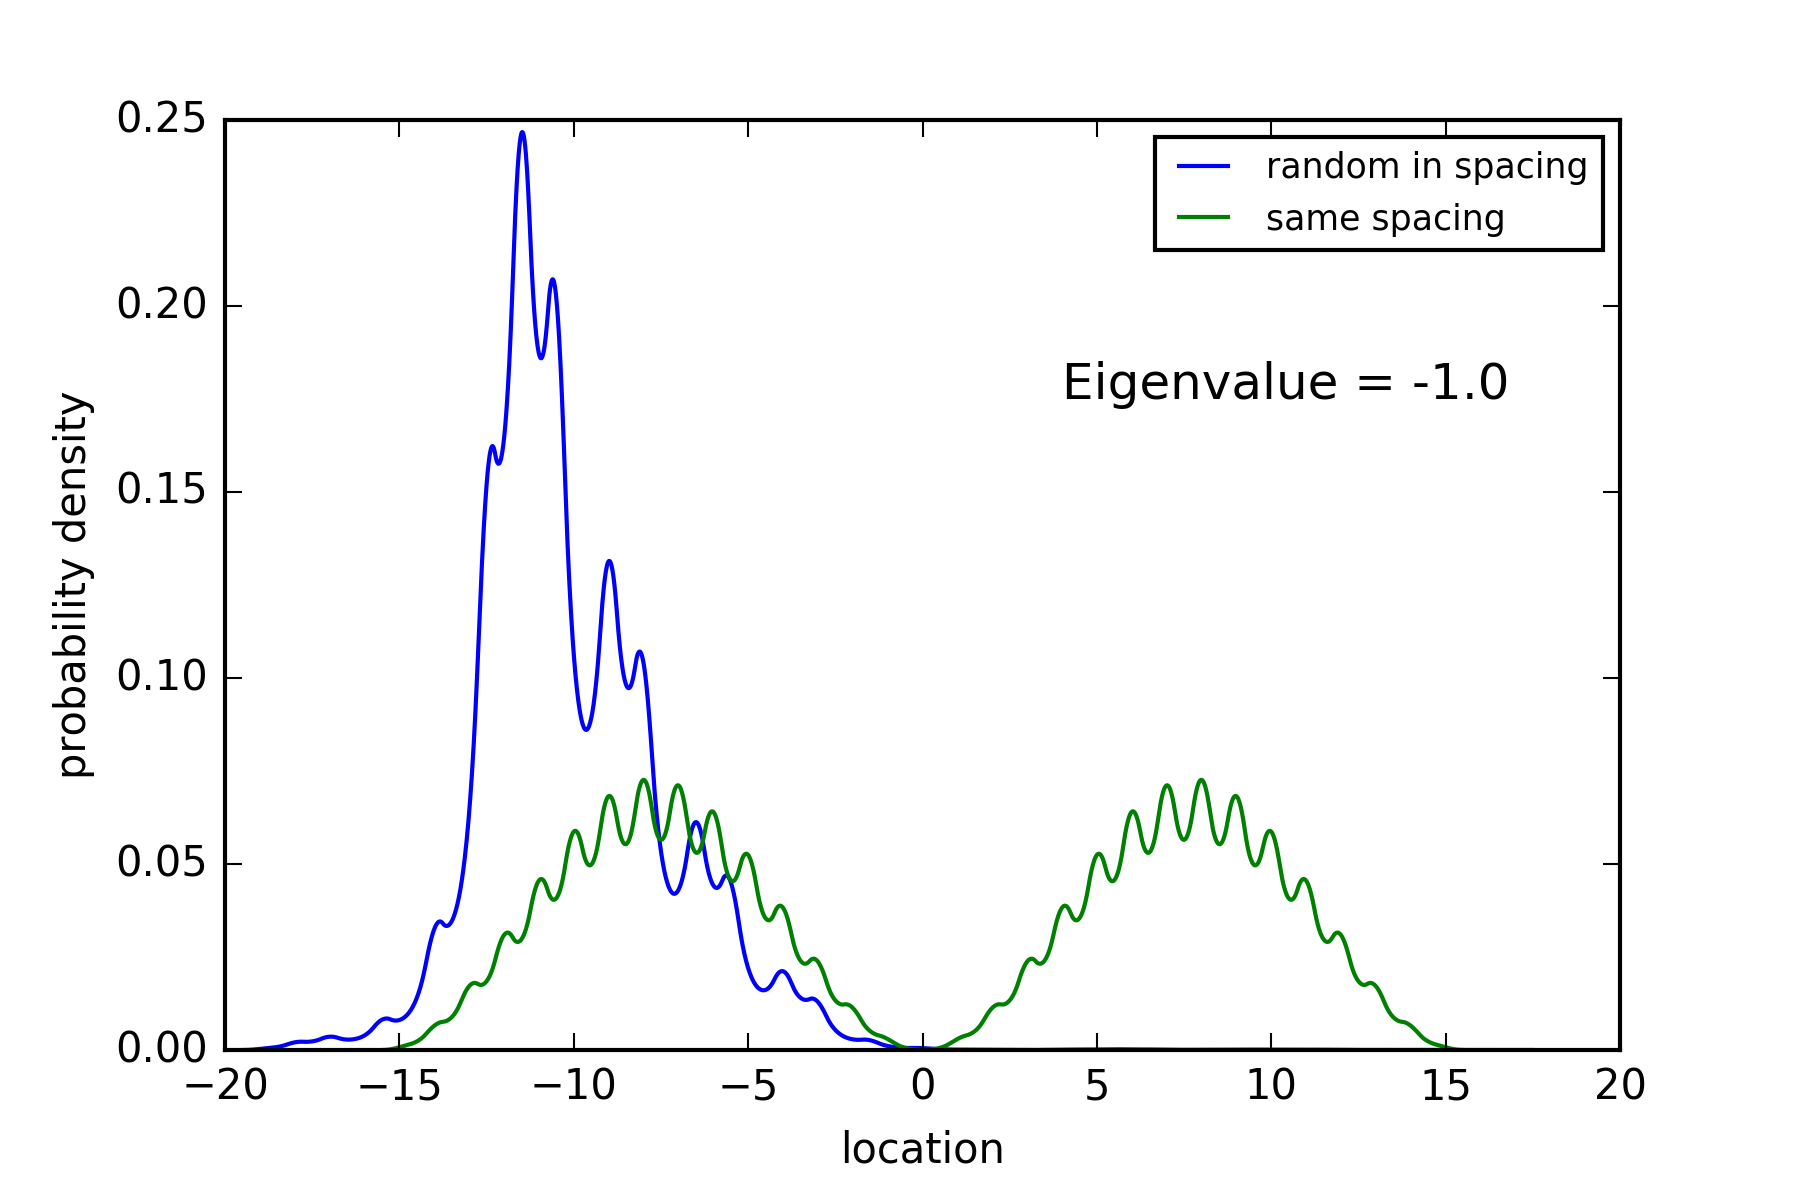
\includegraphics[width=1.1\linewidth]{Graphics/1_0_2th_Lowest_Rand1_5.png}
  \captionof{figure}{2nd Lowest eigenvalue, $V_0l=1.0$, $\{p_1,p_2\}=\{1.5,1.0\}$}
  \label{fig:Area1_2thlowestRand1.5}
\end{minipage}
\end{figure}

%2nd lowest, Vl = 10
\begin{figure}[!htbh]
\centering
\begin{minipage}{.45\textwidth}
  \centering
  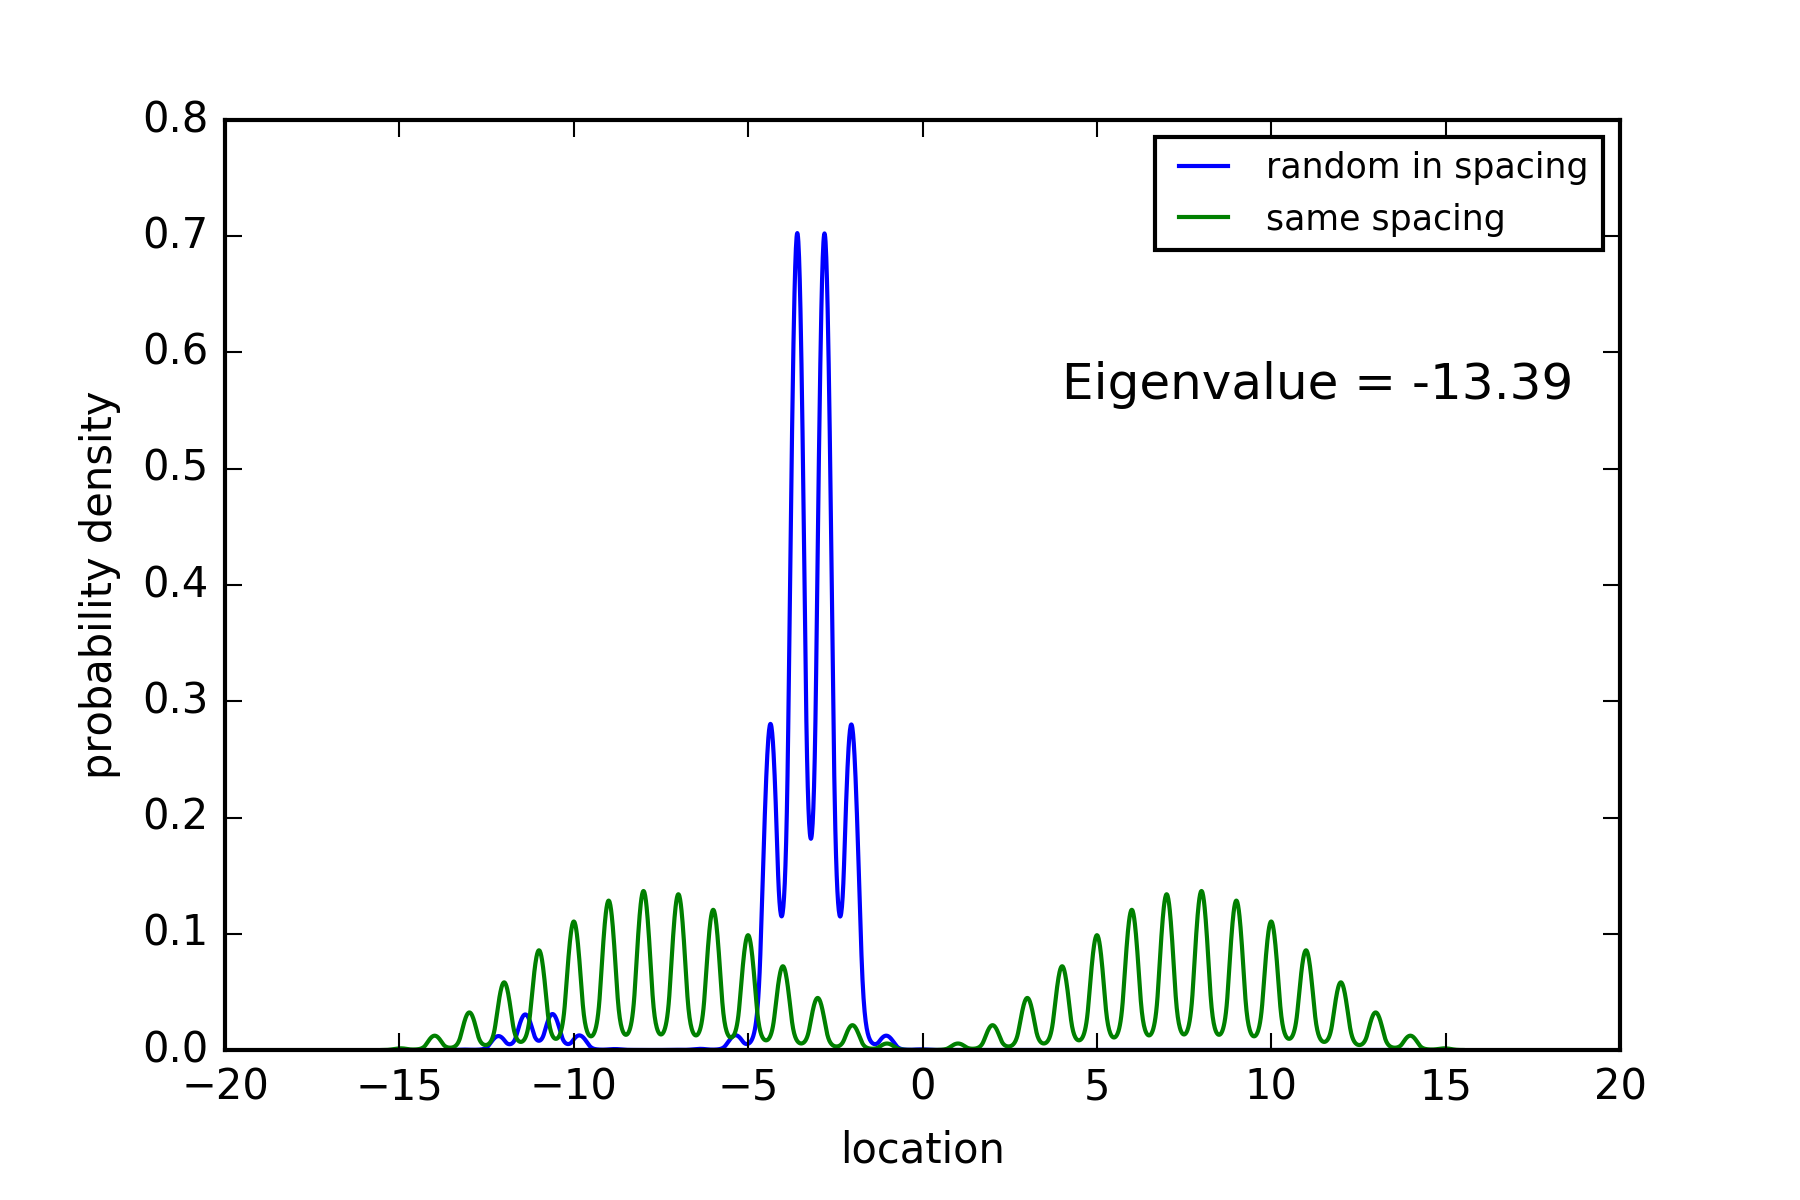
\includegraphics[width=1.1\linewidth]{Graphics/10_0_2th_Lowest_Rand0_8.png}
  \captionof{figure}{2nd Lowest eigenvalue, $V_0l=10.0$, $\{p_1,p_2\}=\{0.8,1.0\}$}
  \label{fig:Area10_2thlowestRand0.8}
\end{minipage}\qquad
\begin{minipage}{.45\textwidth}
  \centering
  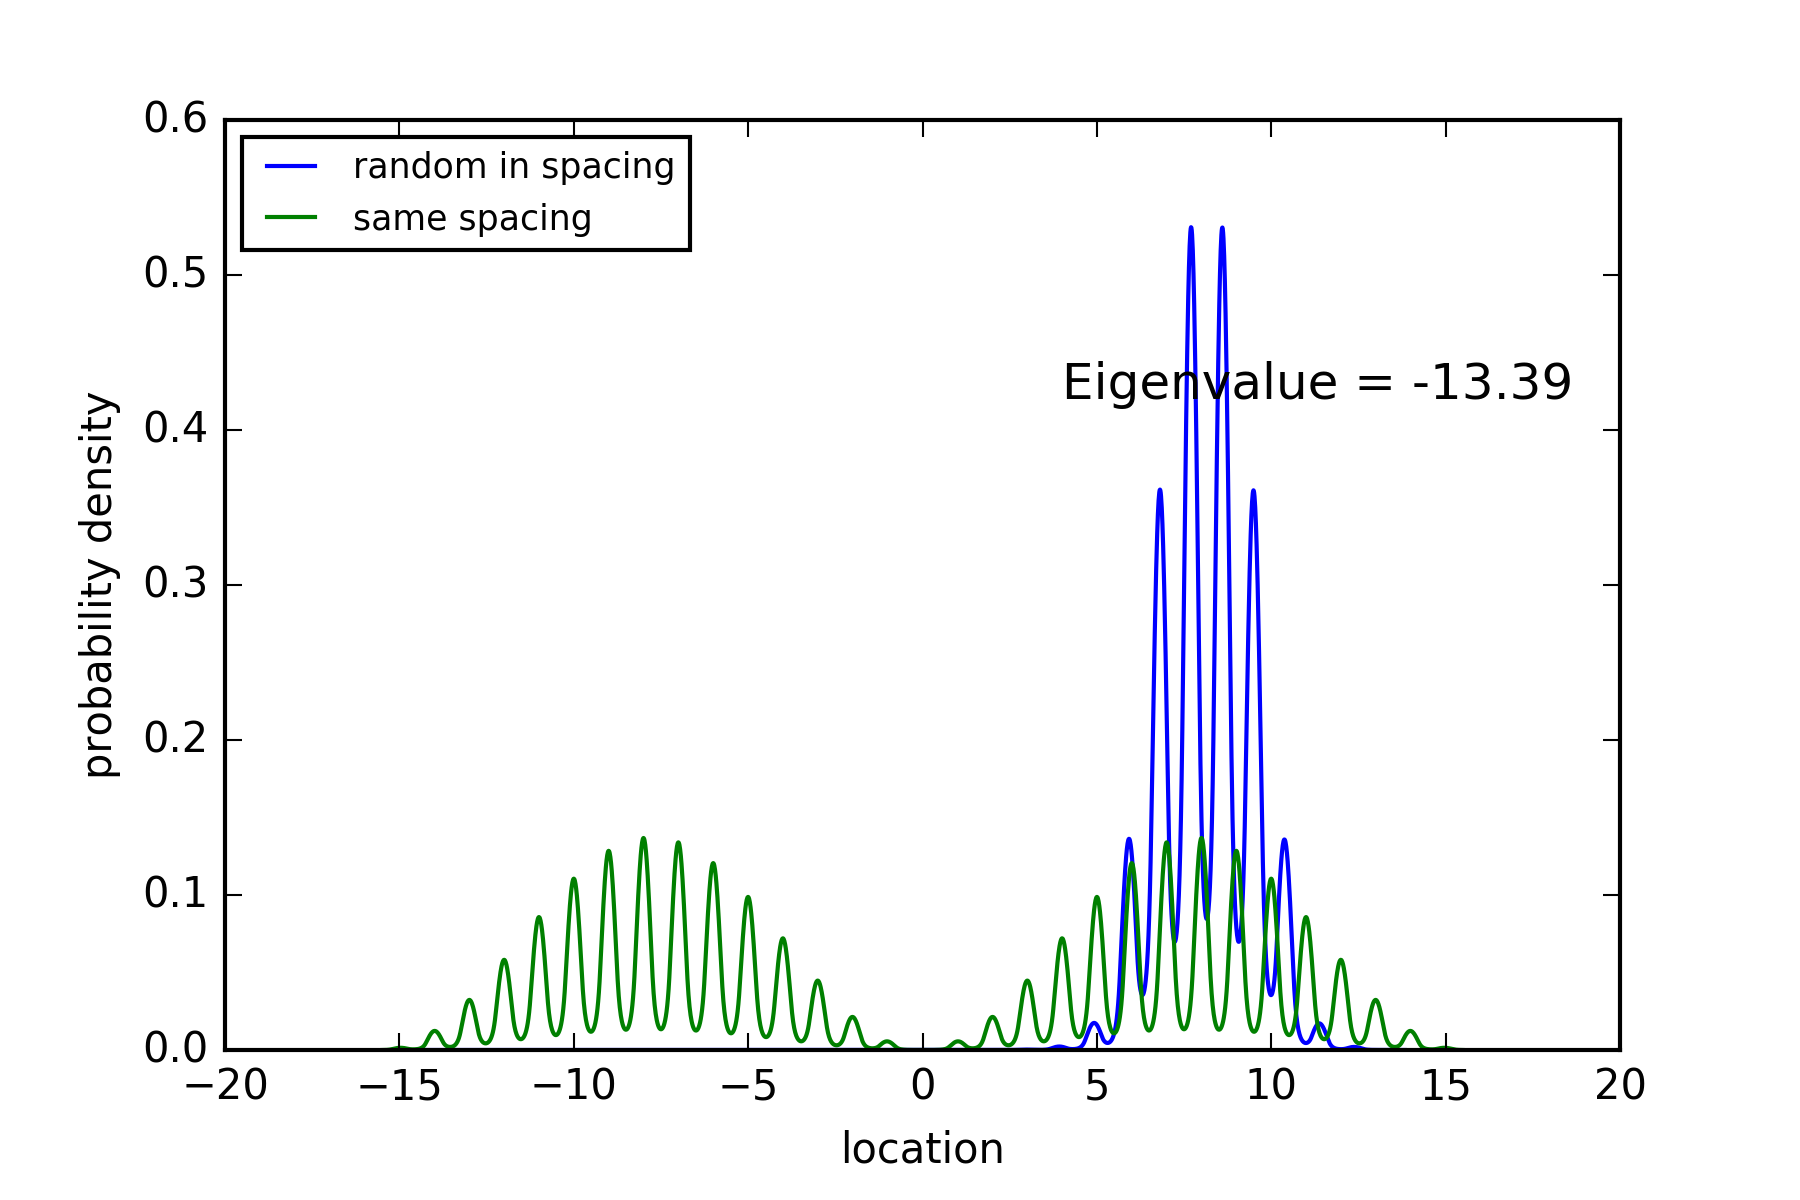
\includegraphics[width=1.1\linewidth]{Graphics/10_0_2th_Lowest_Rand0_9.png}
  \captionof{figure}{2nd Lowest eigenvalue, $V_0l=10.0$,$\{p_1,p_2\}=\{0.9,1.0\}$}
  \label{fig:Area10_2thlowestRand0.9}
\end{minipage}
\end{figure}

\begin{figure}[!htbh]
\centering
\begin{minipage}{.45\textwidth}
  \centering
  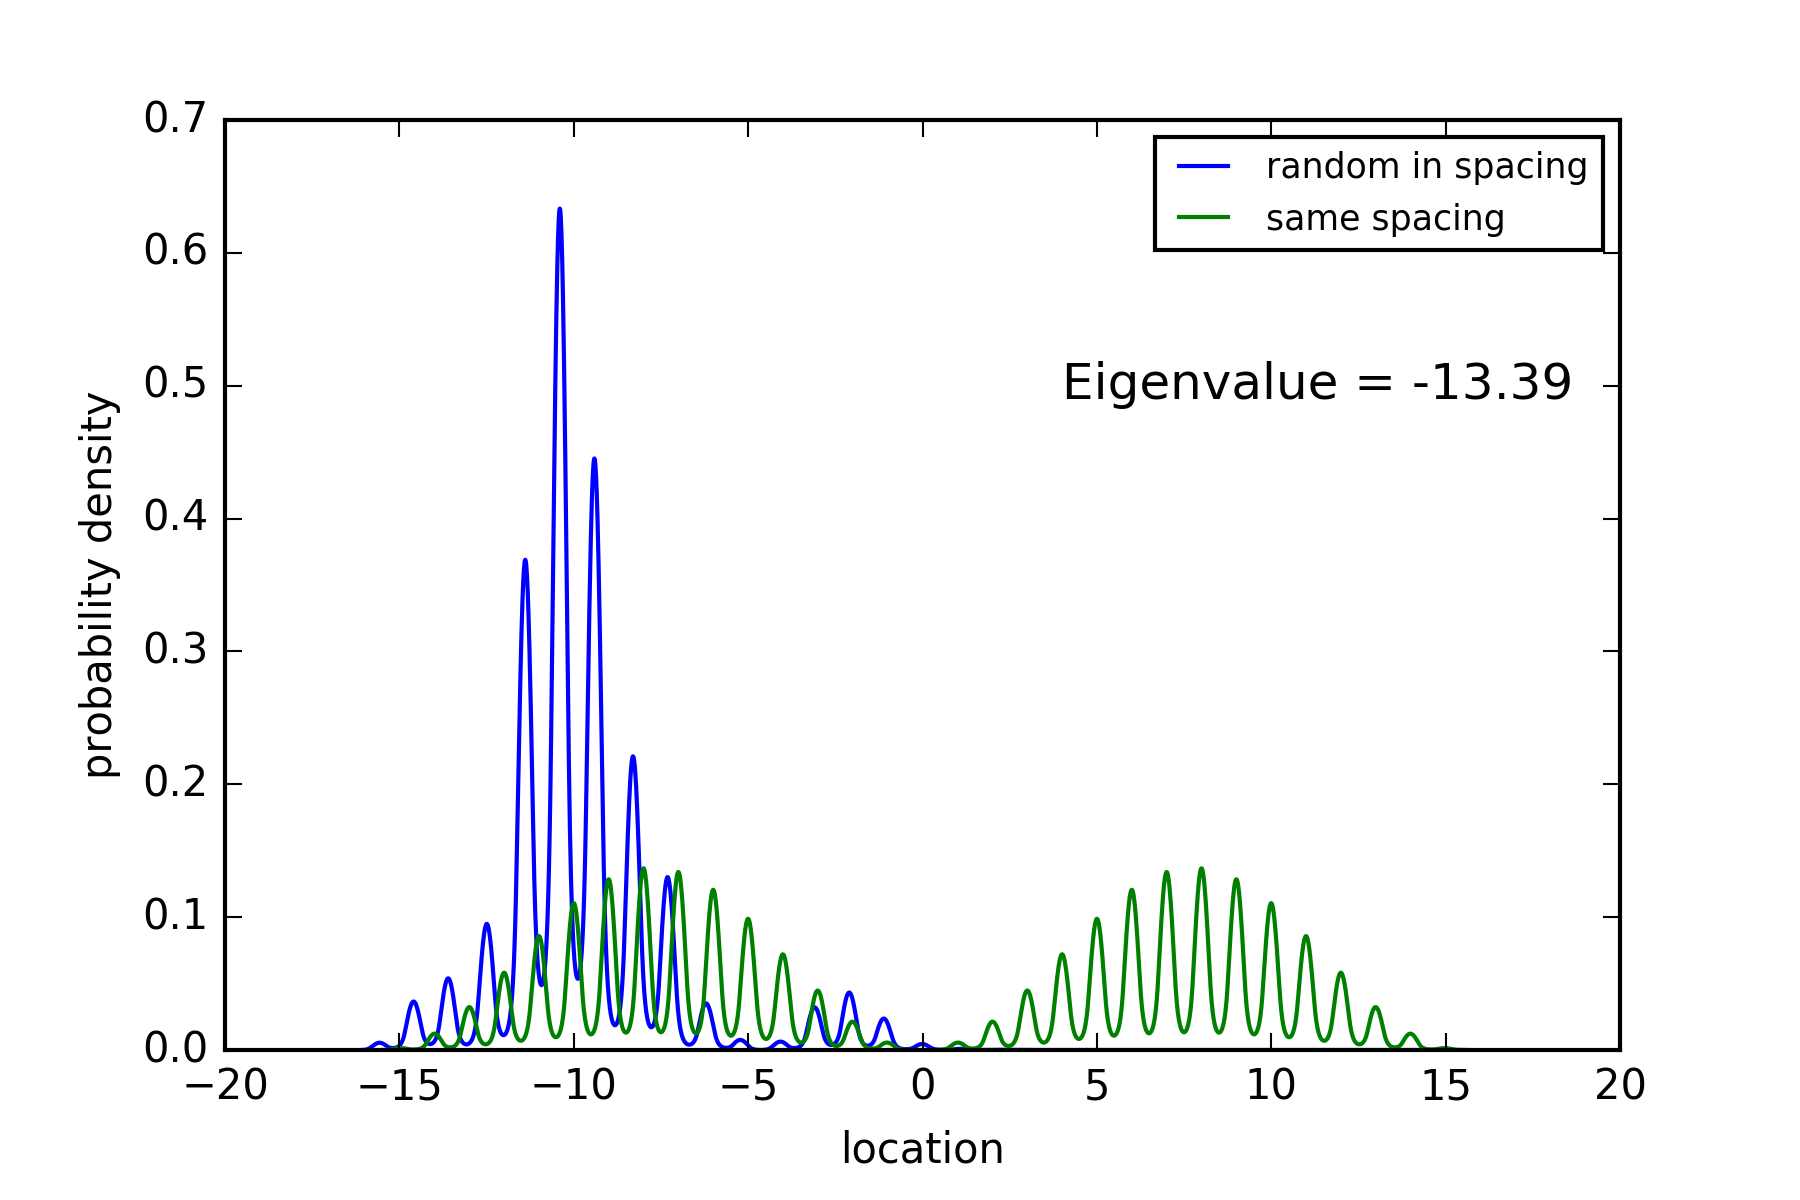
\includegraphics[width=1.1\linewidth]{Graphics/10_0_2th_Lowest_Rand1_1.png}
  \captionof{figure}{2nd Lowest eigenvalue, $V_0l=10.0$, $\{p_1,p_2\}=\{1.1,1.0\}$}
  \label{fig:Area10_2thlowestRand1.1}
\end{minipage}\qquad
\begin{minipage}{.45\textwidth}
  \centering
  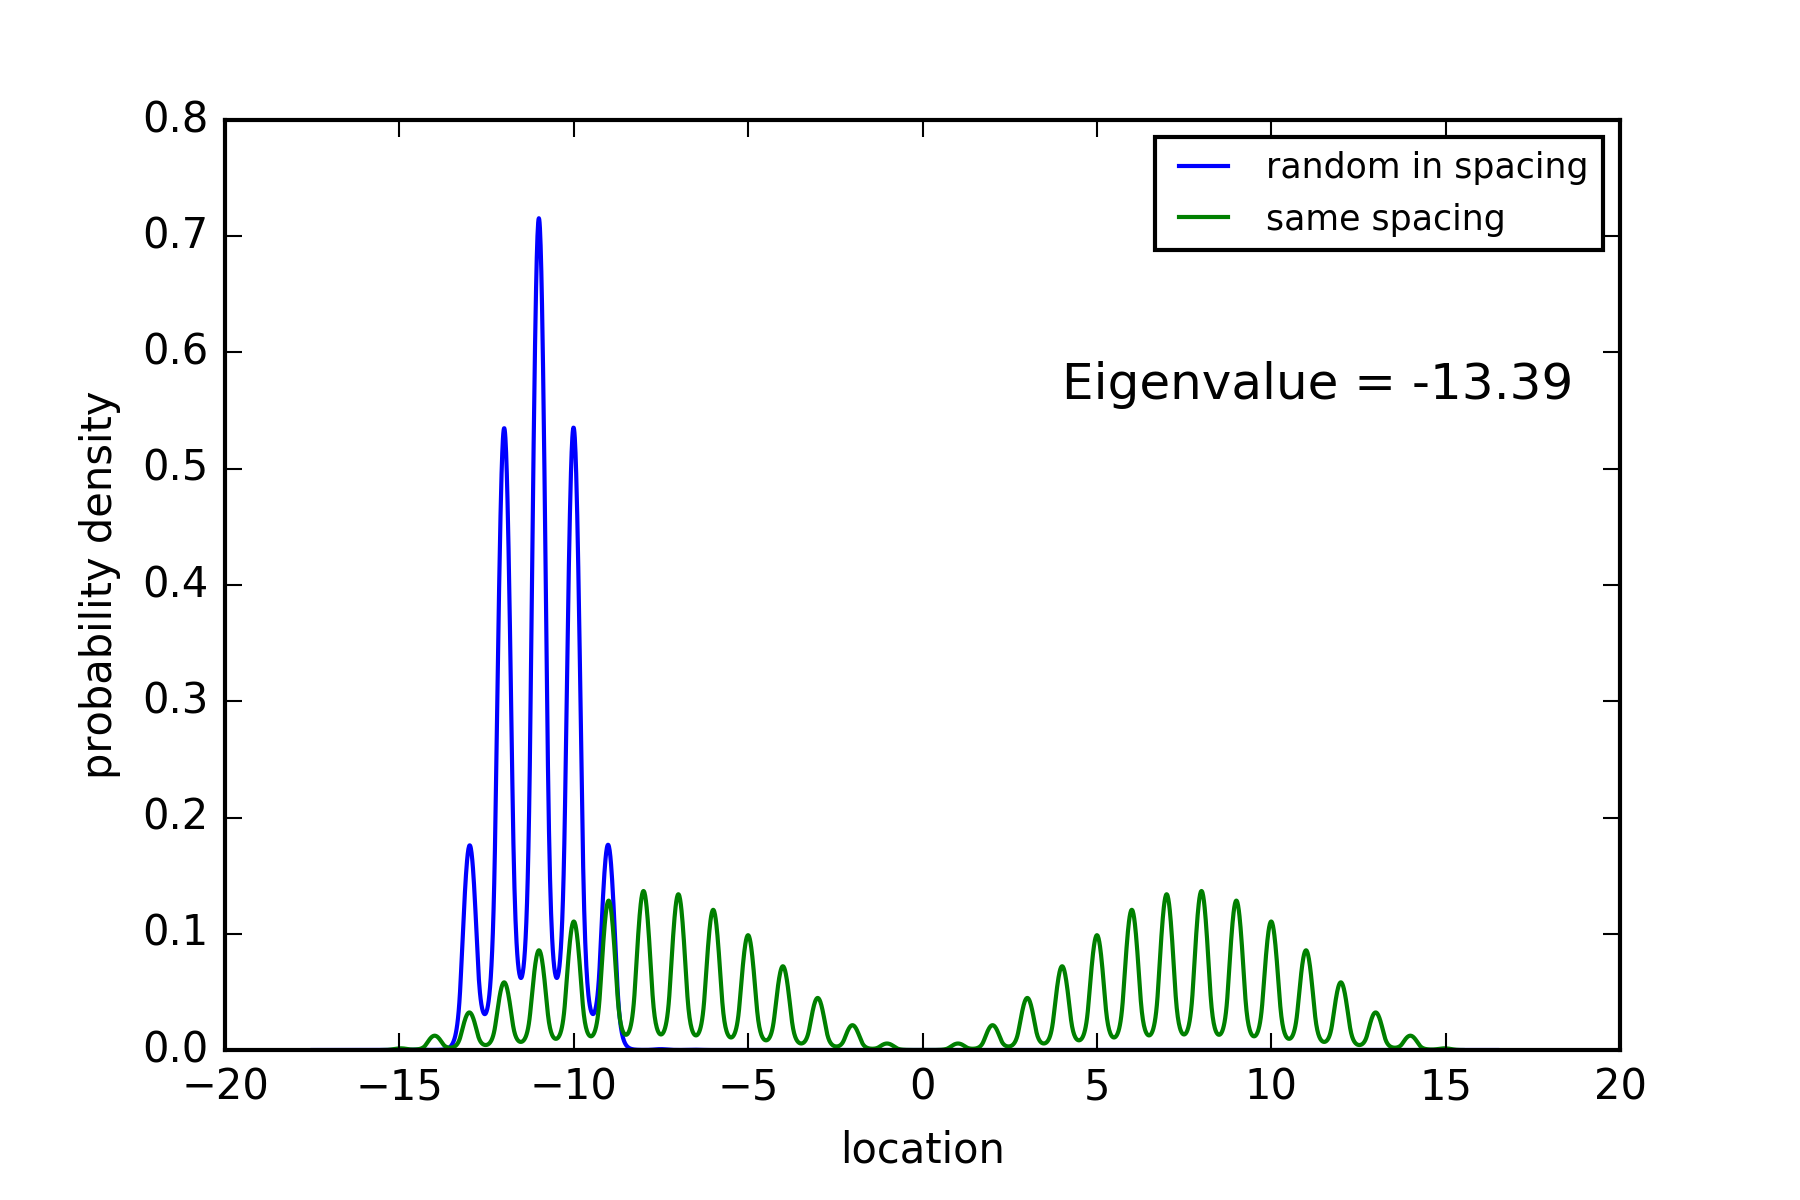
\includegraphics[width=1.1\linewidth]{Graphics/10_0_2th_Lowest_Rand1_5.png}
  \captionof{figure}{2nd Lowest eigenvalue, $V_0l=10.0$, $\{p_1,p_2\}=\{1.5,1.0\}$}
  \label{fig:Area10_2thlowestRand1.5}
\end{minipage}%
\end{figure}

%16:45 modifiled

\newpage
\subsection{Randomness in potential}\label{Randomness in potential}
Since the potential is determined in this model by the potential height and well width, and the product of potential height and well width gives the area of the square potential, we can introduce randomness to this type of system by fixing a value for the area first, and at each atom site, picking a value for the well width from $\{w_1,w_2\}$ with probability $\{0.5,0.5\}$.  For example, for a chain of 5 atoms, we might get a sequence of well widths, ${0.2,0.5,0.5,0.2,0.2}$ if we are allowed to pick from $\{0.2,0.5\}$. With area given, say 1.0, we are can get a sequence of potential heights for the atoms, {5,2,,2,5,5}. Hence these two sequences define the non-overlapping square potential at each atom site for this system of 5 atoms. 

The following figures are probability density function corresponding to first and second lowest eigenenergies when $V_0l$ is equal to 1 or 2 or 5, with well width picked from $\{w_1,w_2\}$ with probability of $\{0.5,0.5\}$.

%lowest vl = 1.0

\begin{figure}[!htbh]
\centering
\begin{minipage}{.45\textwidth}
  \centering
  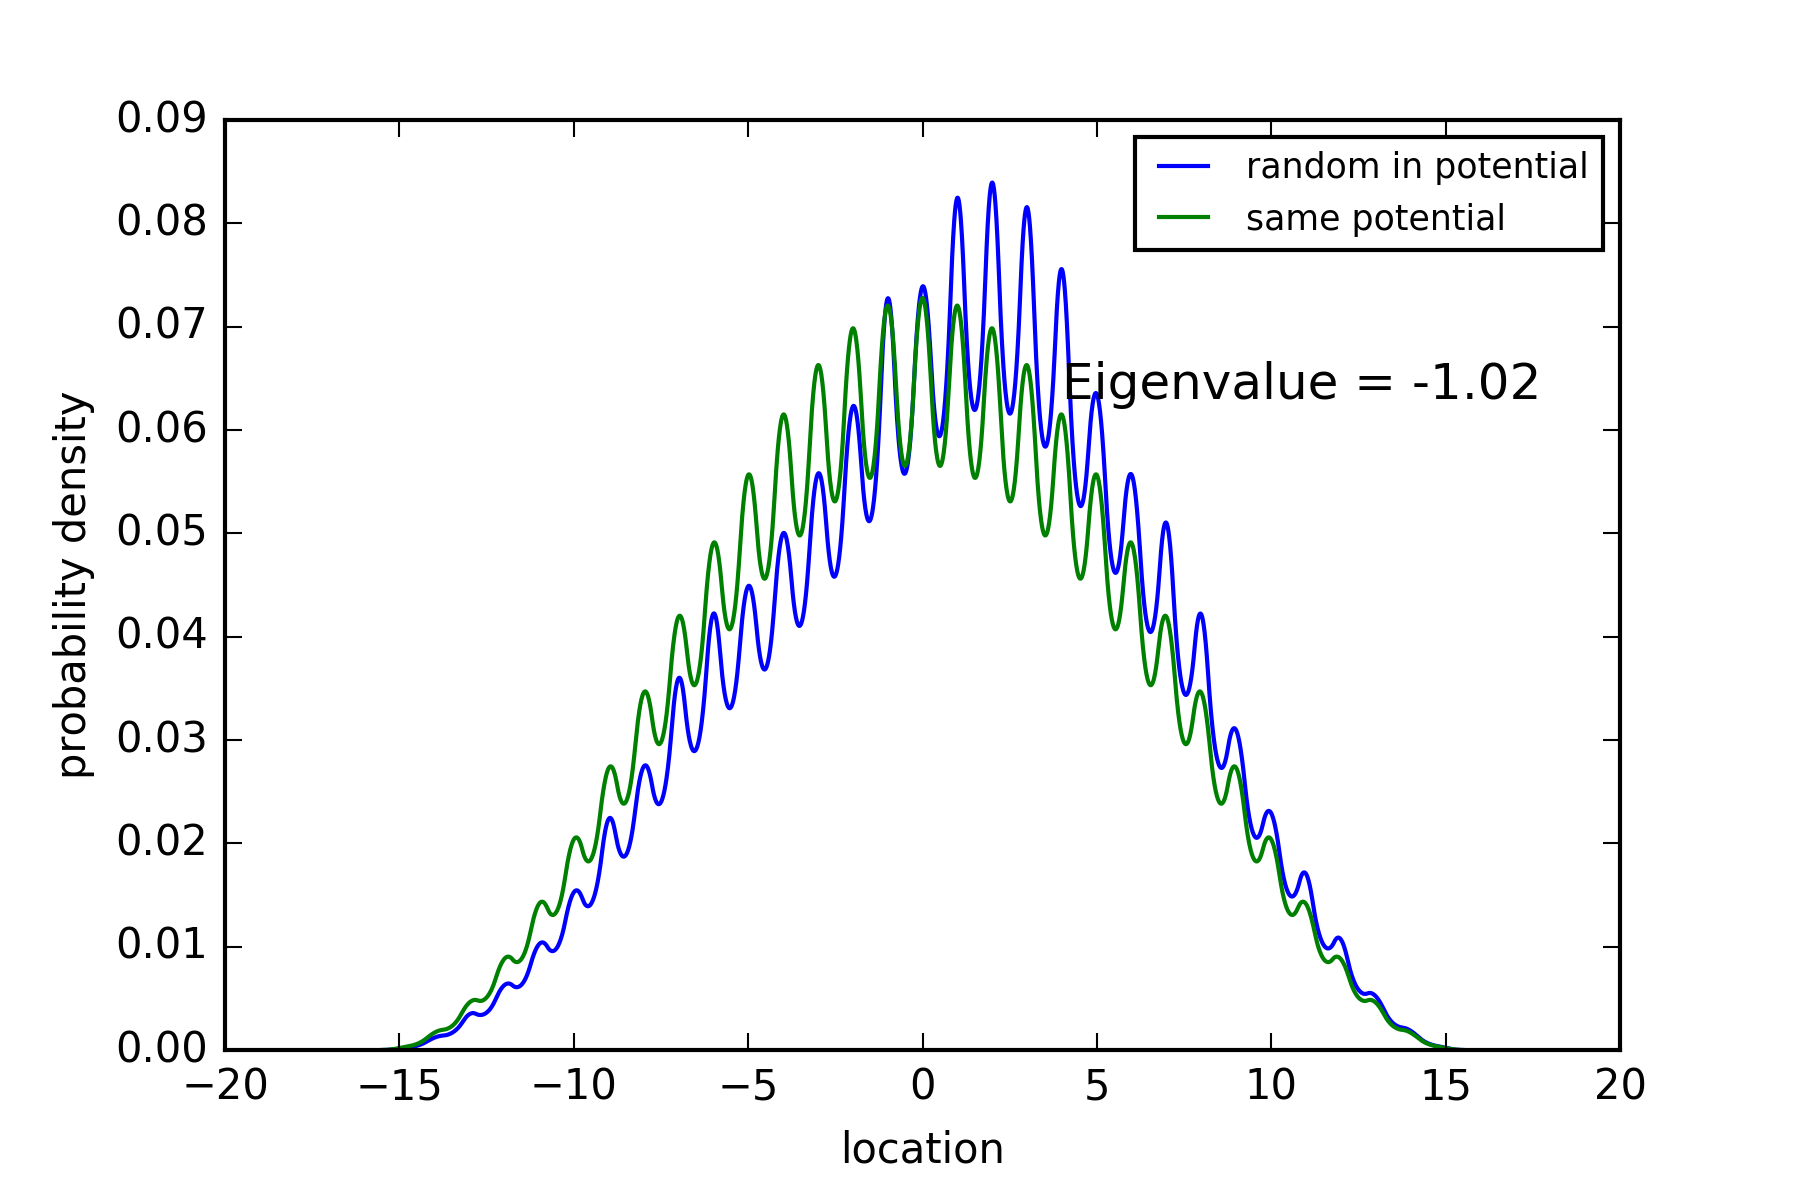
\includegraphics[width=1.1\linewidth]{RandomPotential2/1_0a_1th_Lowest_Rand0_4_0_5.png}
  \captionof{figure}{Lowest eigenvalue, $V_0l =1.0$ , $w_1 = 0.4 $,$w_2 = 0.5$ }
  \label{fig:randPoa1_1th_0.5_0.4}
\end{minipage}\qquad
\begin{minipage}{.45\textwidth}
  \centering
  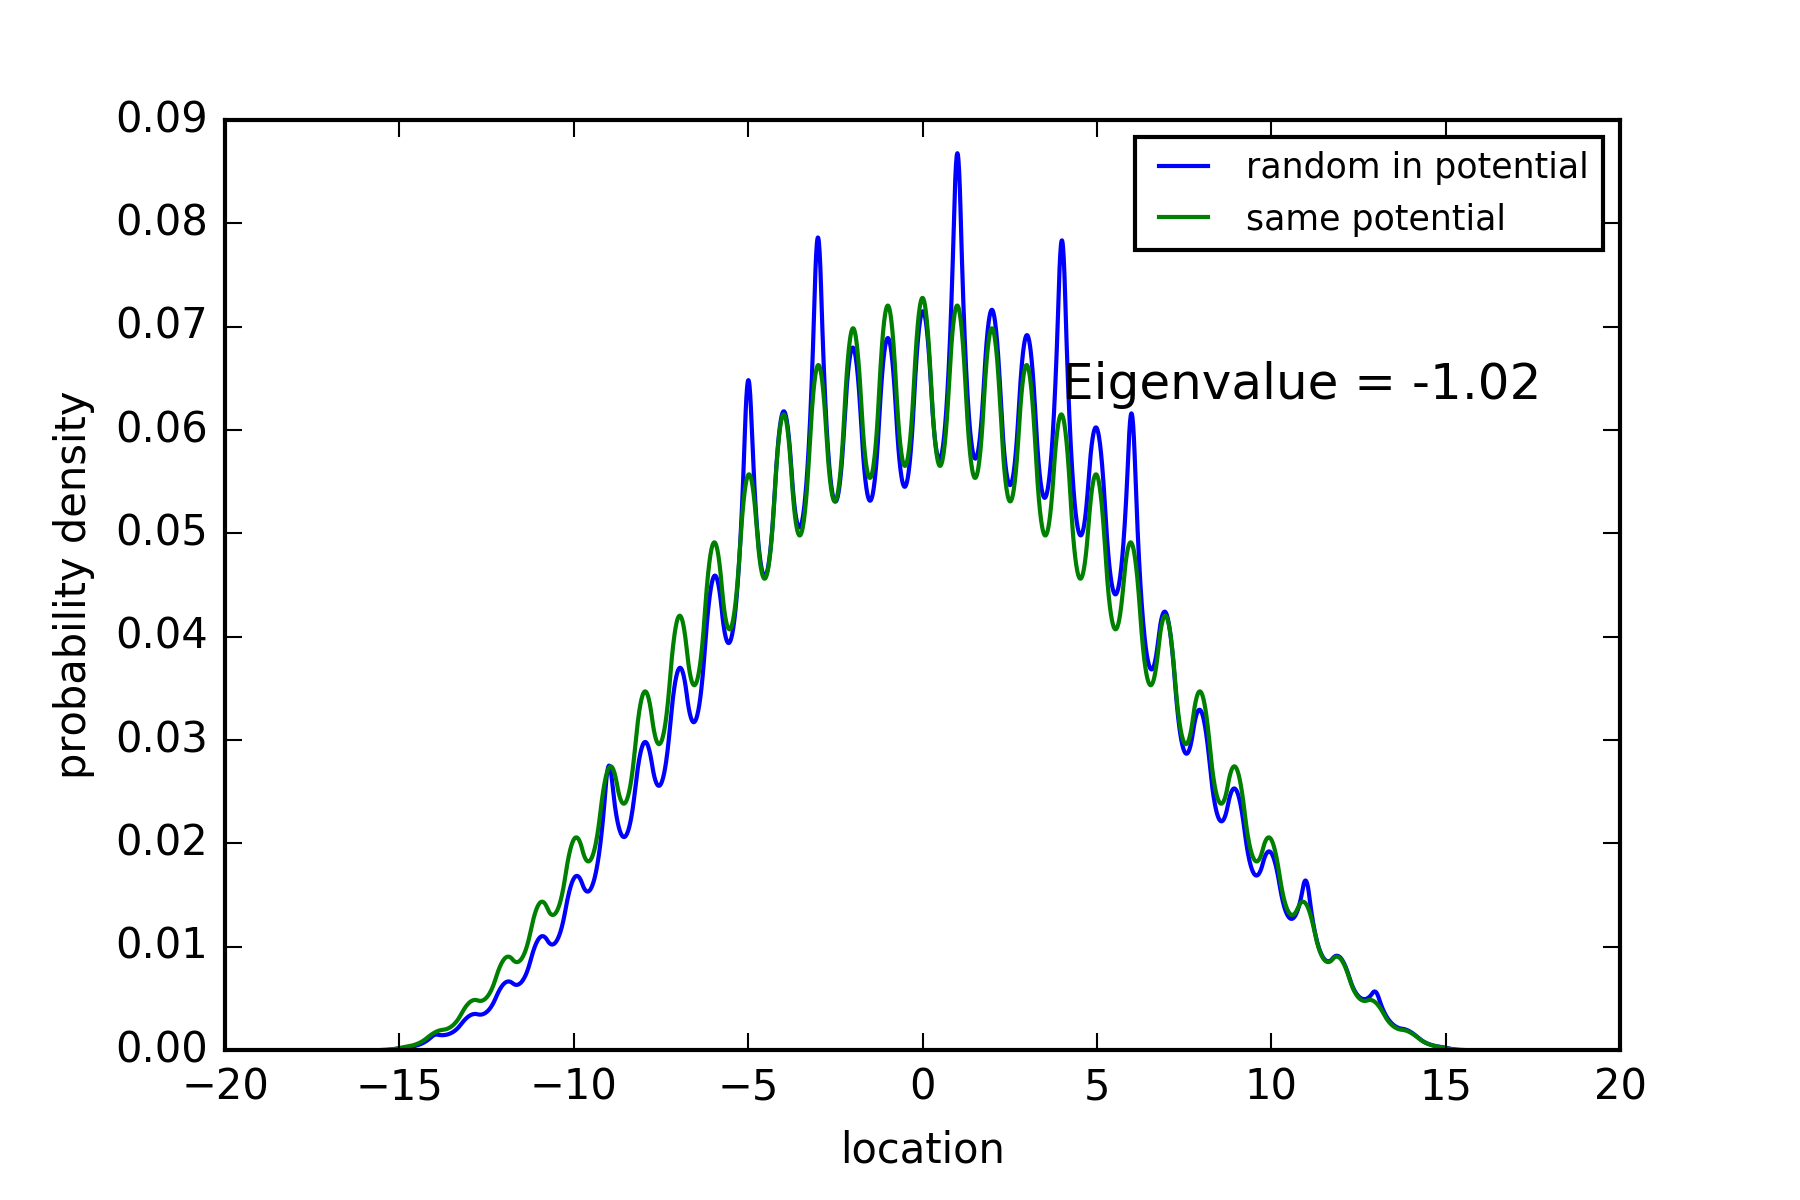
\includegraphics[width=1.1\linewidth]{RandomPotential2/1_0a_1th_Lowest_Rand0_2_0_5.png}
  \captionof{figure}{Lowest eigenvalue, $V_0l=1.0$, $w_1 = 0.2 $, $w_2 = 0.5 $}
  \label{fig:randPoa1_1th_0.5_0.2}
\end{minipage}
\end{figure}

%2nd lowest vl = 1.0
\begin{figure}[!htbh]
\centering
\begin{minipage}{.45\textwidth}
  \centering
  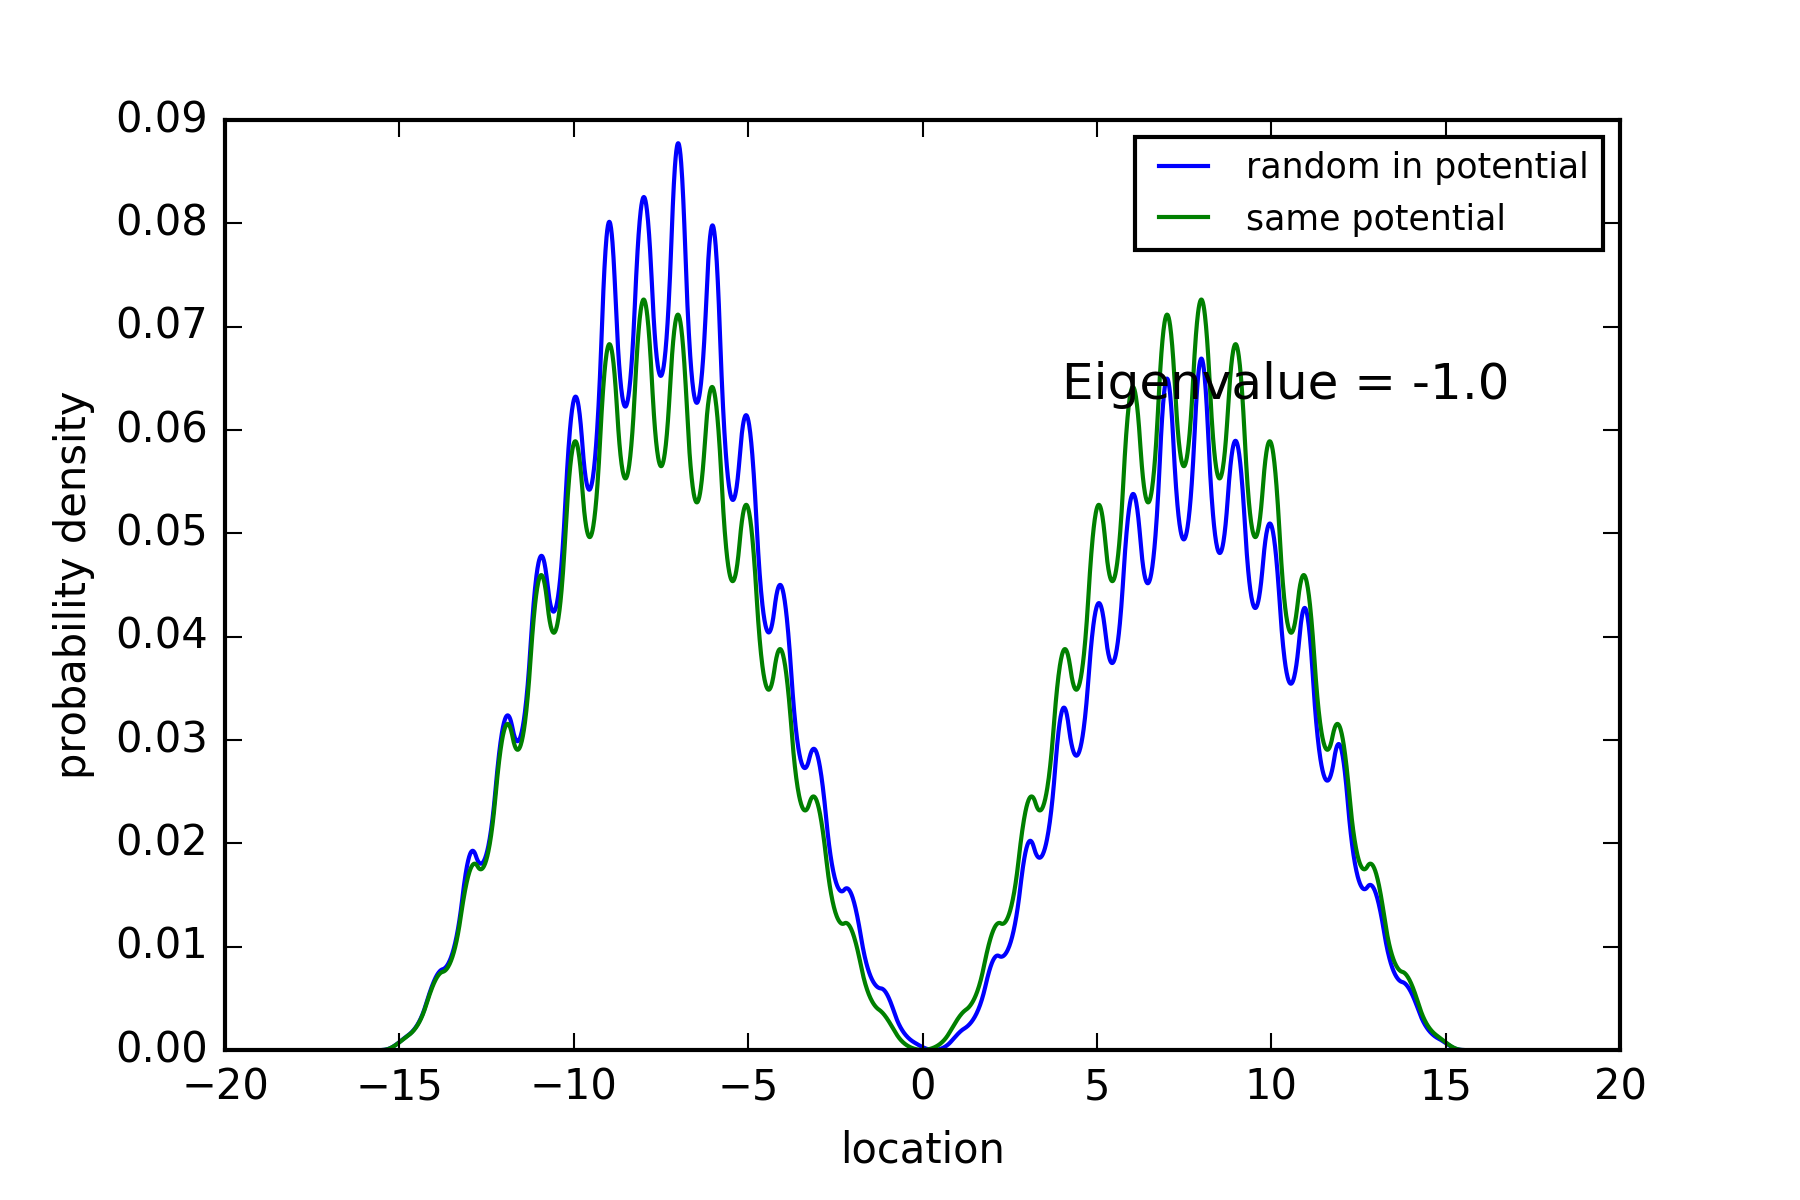
\includegraphics[width=1.1\linewidth]{RandomPotential2/1_0a_2th_Lowest_Rand0_4_0_5.png}
  \captionof{figure}{Lowest eigenvalue $V_0l$=1.0, $w_1 = 0.4 $,$w_2 = 0.5$}
  \label{fig:randPoa1_2th_0.5_0.4}
\end{minipage}\qquad
\begin{minipage}{.45\textwidth}
  \centering
  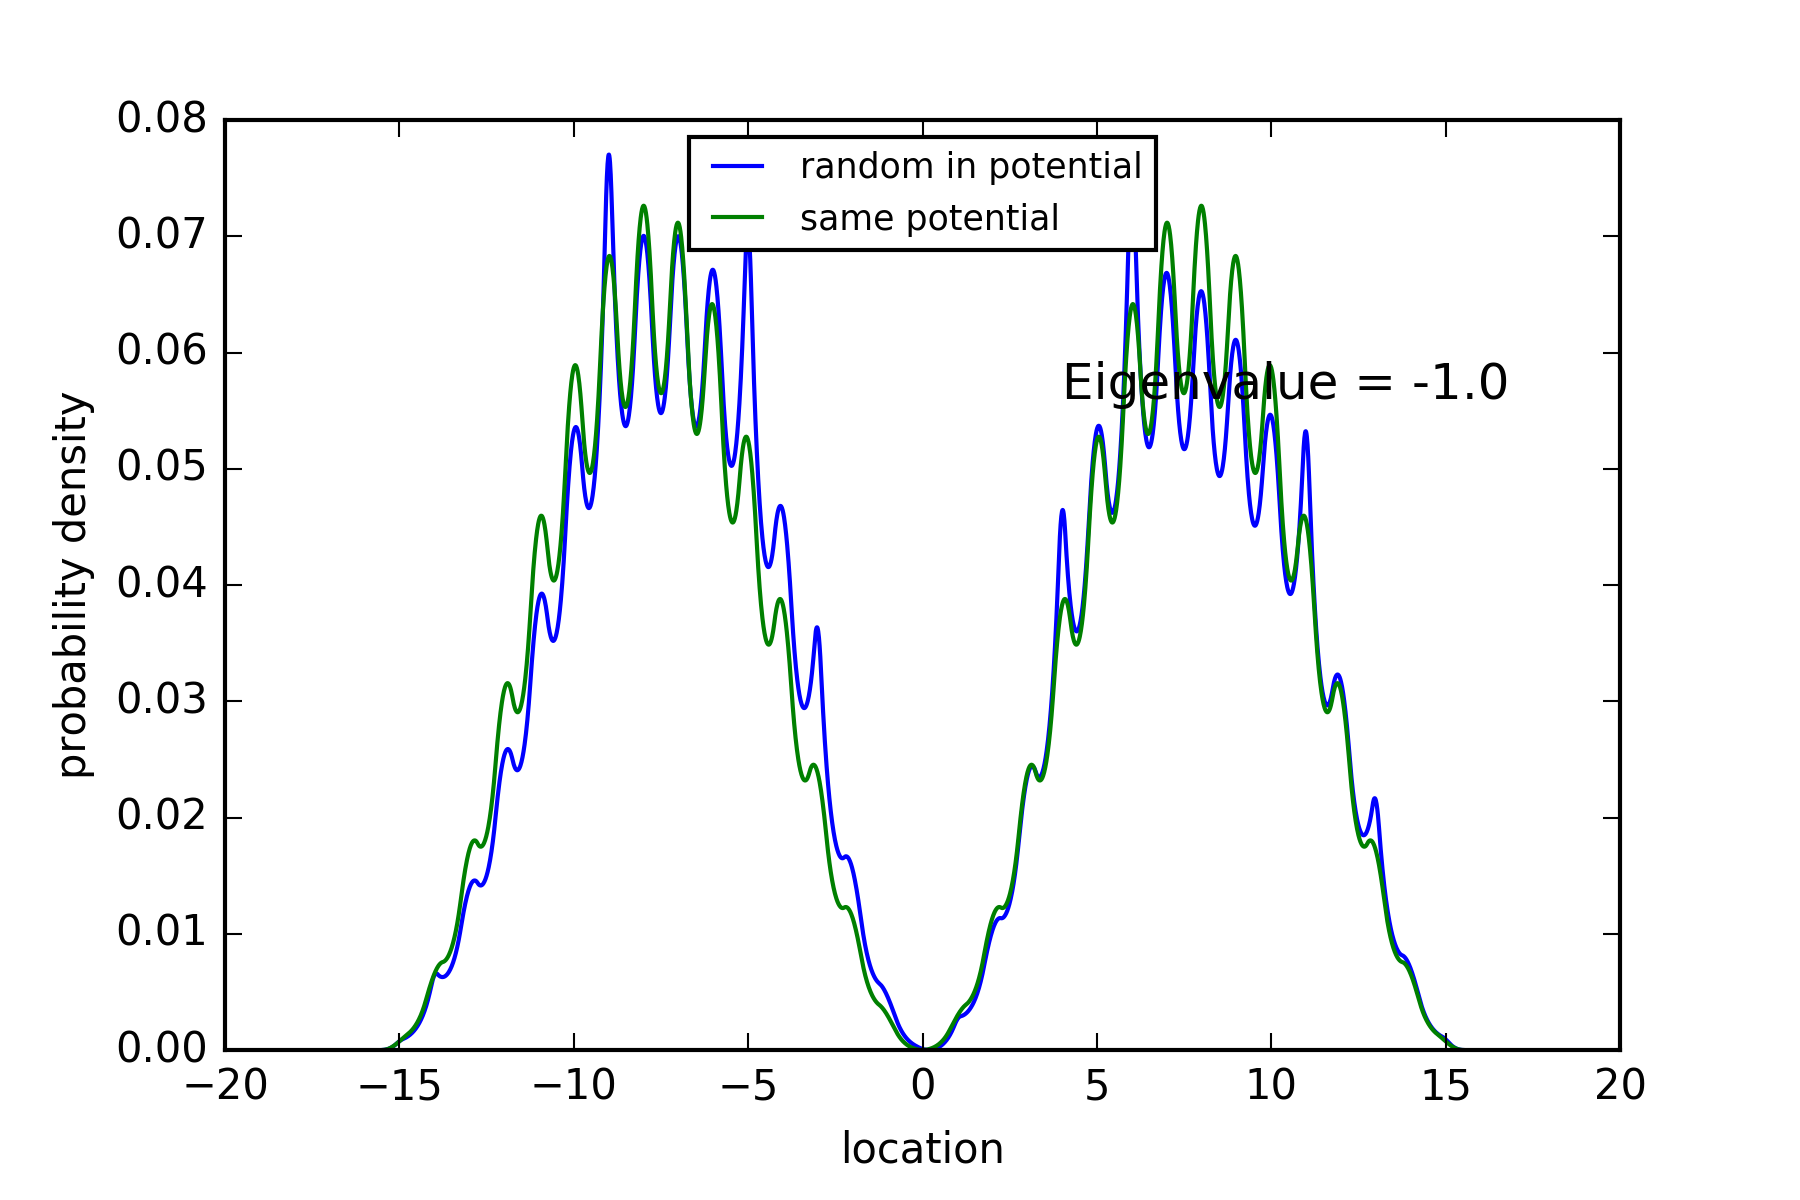
\includegraphics[width=1.1\linewidth]{RandomPotential2/1_0a_2th_Lowest_Rand0_2_0_5.png}
  \captionof{figure}{Lowest eigenvalue, $V_0l=1.0$,$w_1 = 0.2 $, $w_2 = 0.5 $}
  \label{fig:randPoa1_2th_0.5_0.4}
\end{minipage}
\end{figure}

%lowest vl = 5.0
\begin{figure}[!htbh]
\centering
\begin{minipage}{.45\textwidth}
  \centering
  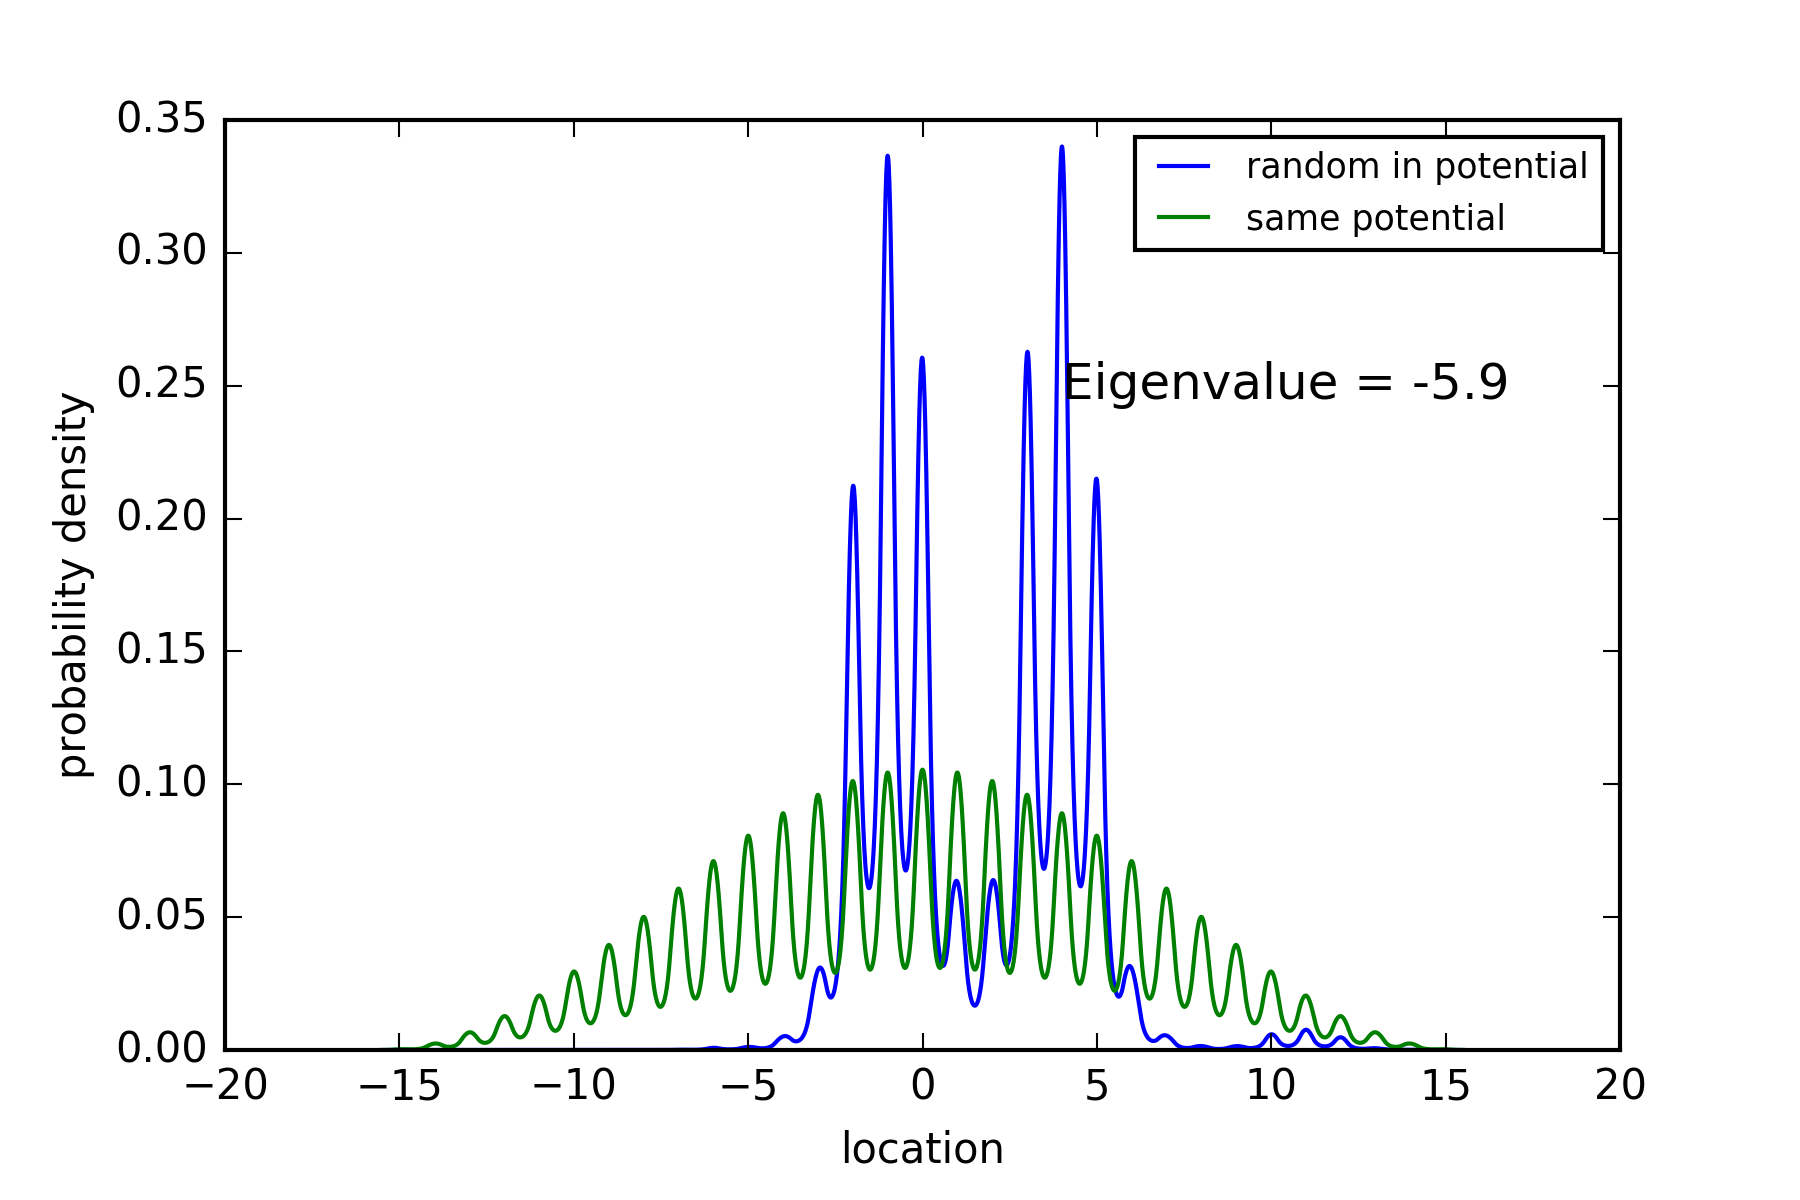
\includegraphics[width=1.1\linewidth]{RandomPotential2/5_0a_1th_Lowest_Rand0_4_0_5.png}
  \captionof{figure}{Lowest eigenvalue $V_0l=5.0$, $w_1 = 0.4 $,$w_2 = 0.5$}
  \label{fig:randPoa5_1th_0.5_0.4}
\end{minipage}\qquad
\begin{minipage}{.45\textwidth}
  \centering
  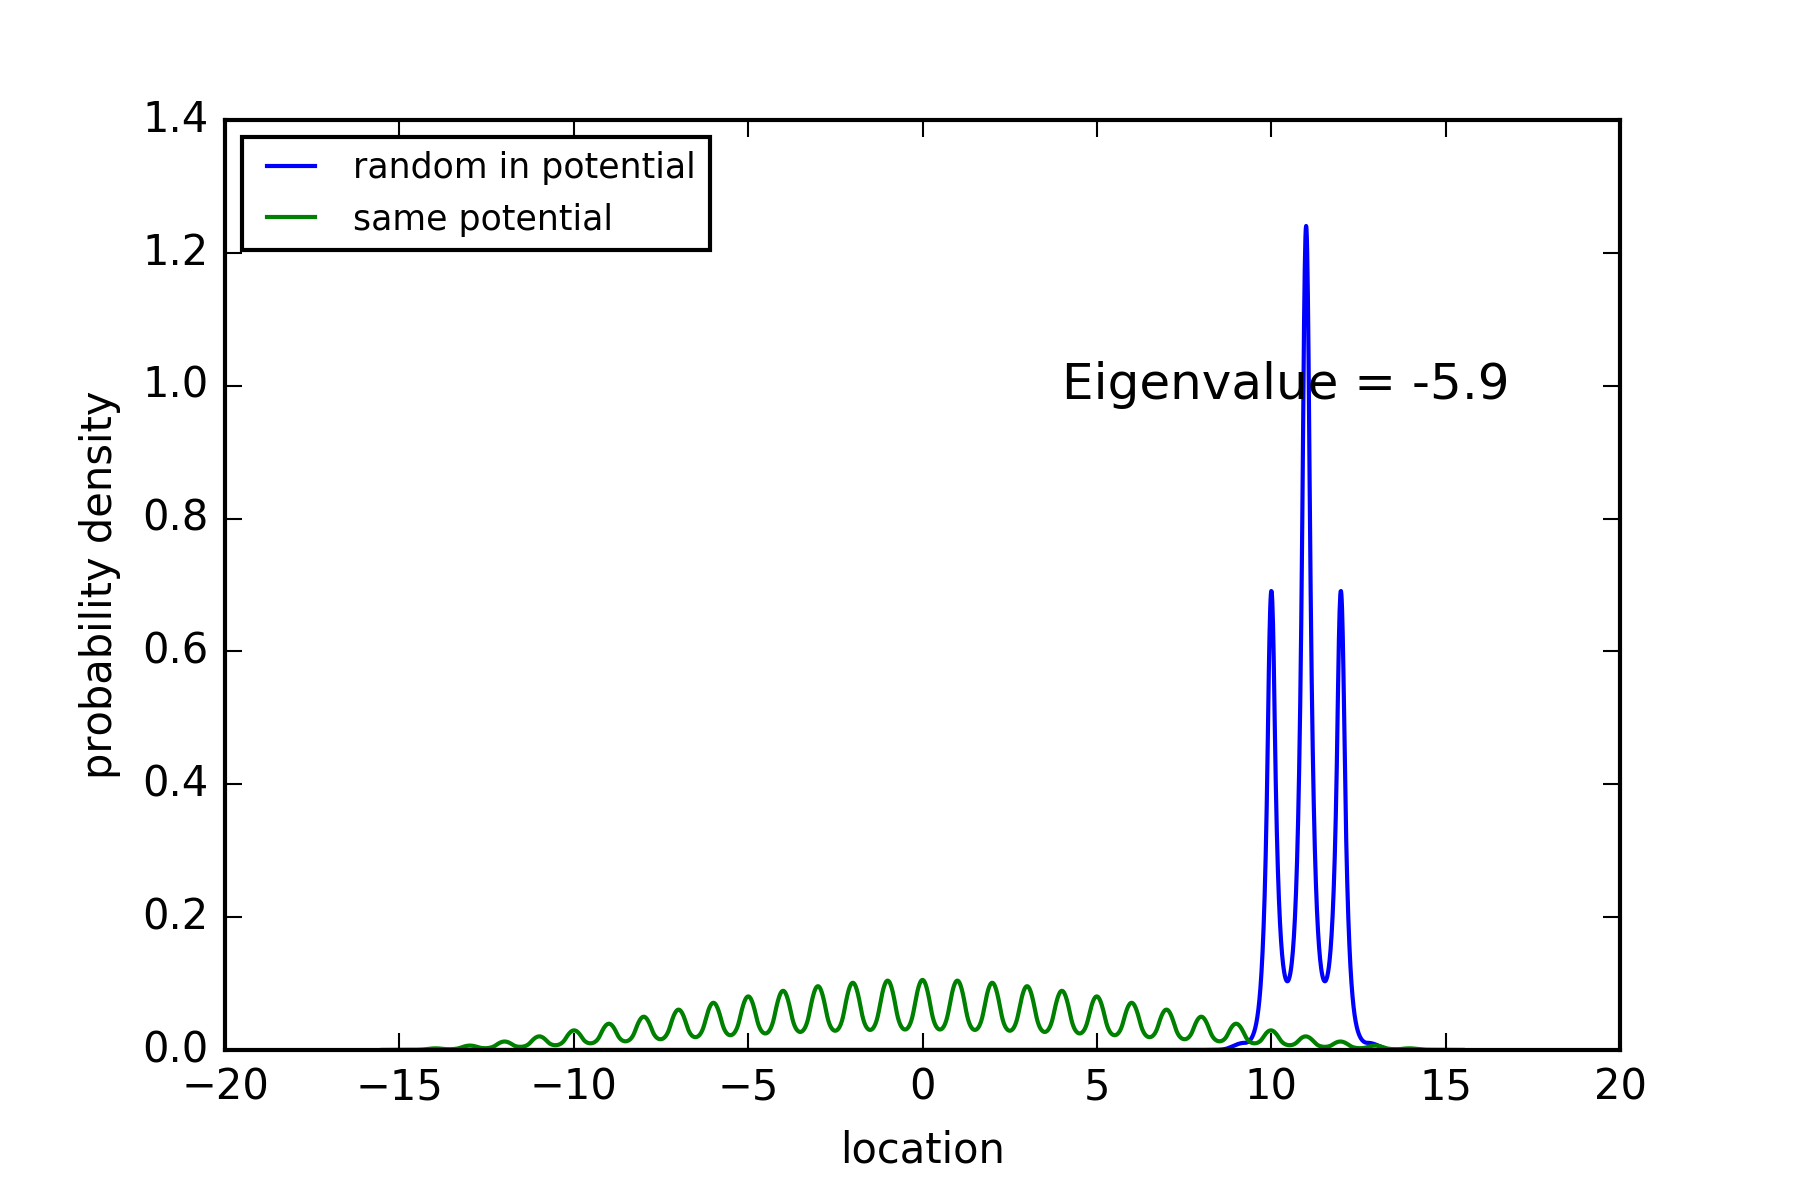
\includegraphics[width=1.1\linewidth]{RandomPotential2/5_0a_1th_Lowest_Rand0_2_0_5.png}
  \captionof{figure}{Lowest eigenvalue $V_0l=5.0$, $w_1 = 0.2 $, $w_2 = 0.5 $}
  \label{fig:randPoa5_1th_0.5_0.2}
\end{minipage}
\end{figure}

%2nd lowest vl = 5.0
\begin{figure}[!htbh]
\centering
\begin{minipage}{.45\textwidth}
  \centering
  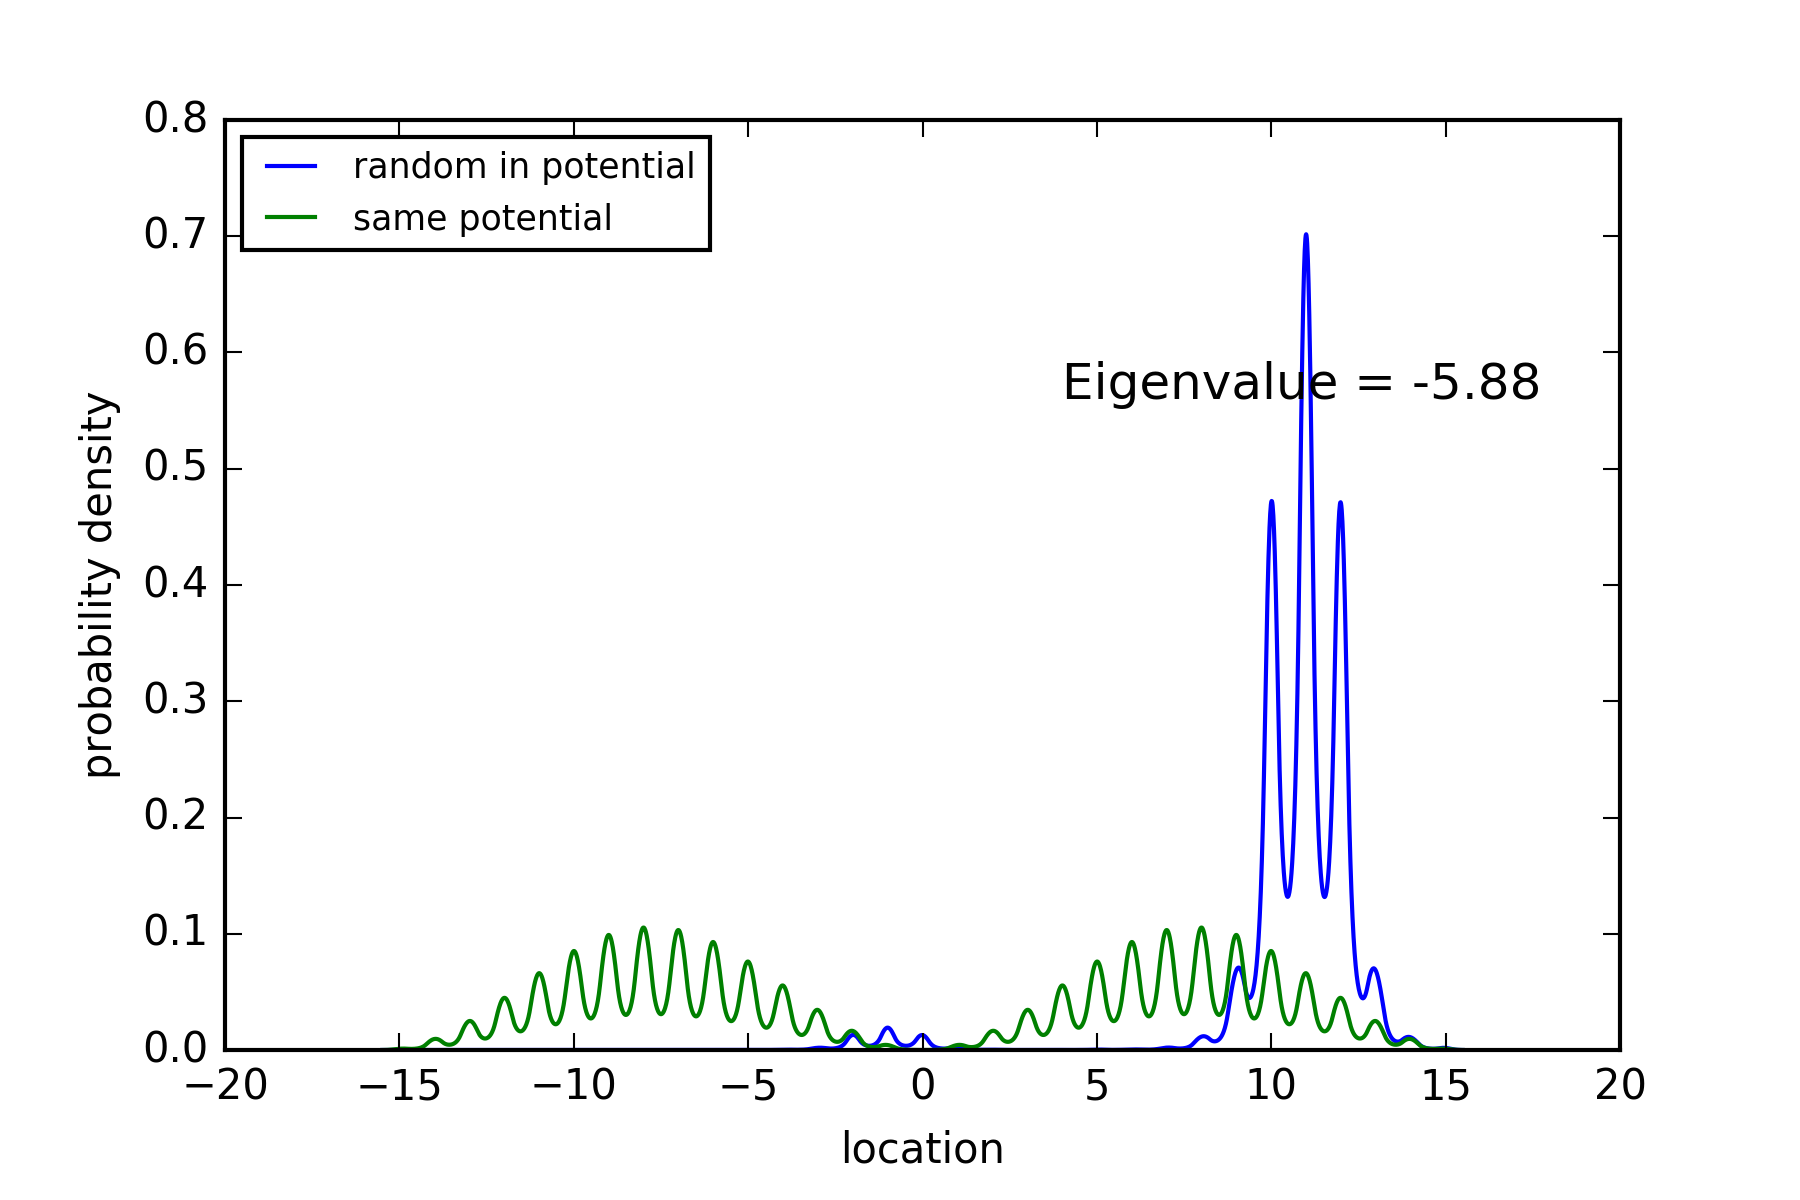
\includegraphics[width=1.1\linewidth]{RandomPotential2/5_0a_2th_Lowest_Rand0_4_0_5.png}
  \captionof{figure}{2nd Lowest eigenvalue, $V_0l=5.0$, $w_1 = 0.4 $,$w_2 = 0.5$}
  \label{fig:randPoa5_2th_0.5_0.4}
\end{minipage}\qquad
\begin{minipage}{.45\textwidth}
  \centering
  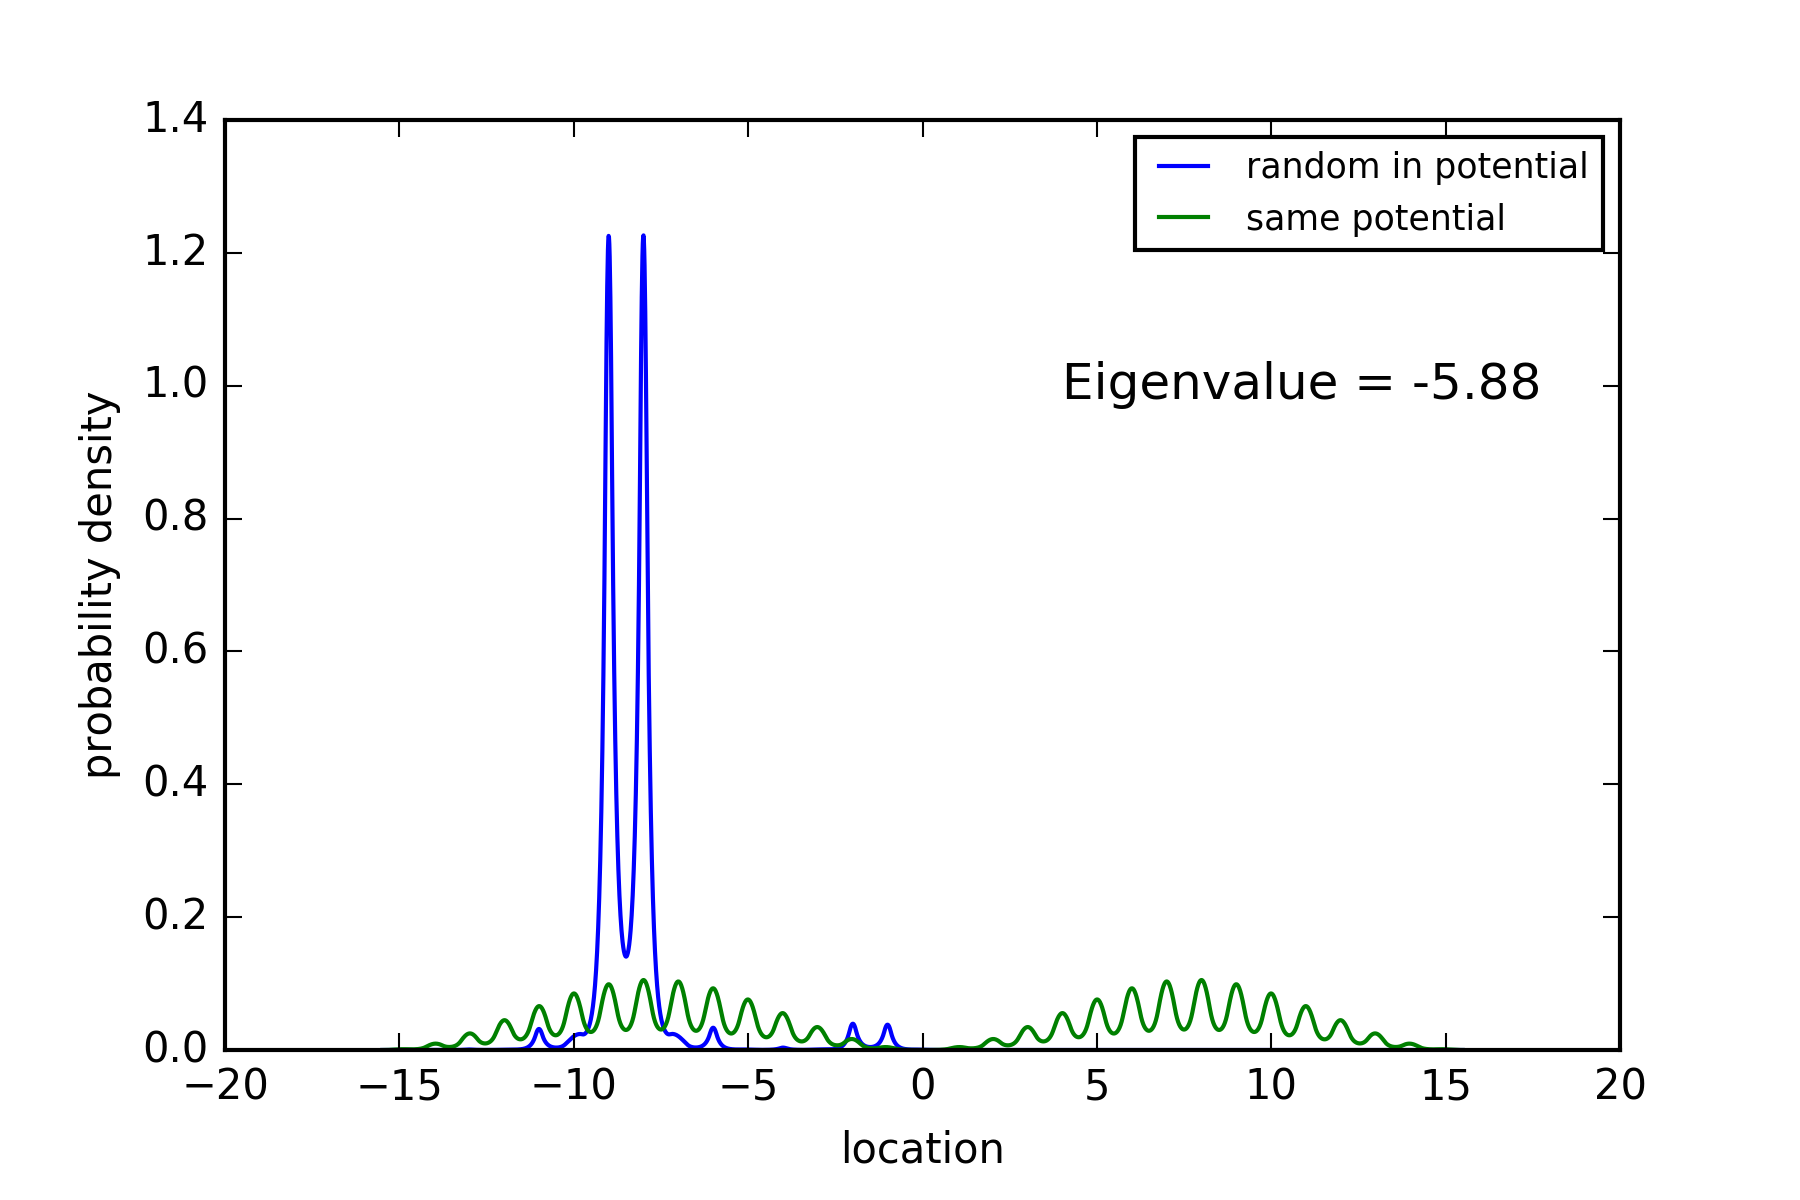
\includegraphics[width=1.1\linewidth]{RandomPotential2/5_0a_2th_Lowest_Rand0_2_0_5.png}
  \captionof{figure}{2nd Lowest eigenvalue, $V_0l=5.0$, $w_1 = 0.2 $, $w_2 = 0.5 $}
  \label{fig:randPoa5_2th_0.5_0.2}
\end{minipage}
\end{figure}

\newpage
%lowest vl = 10.0
\begin{figure}[!htbh]
\centering
\begin{minipage}{.45\textwidth}
  \centering
  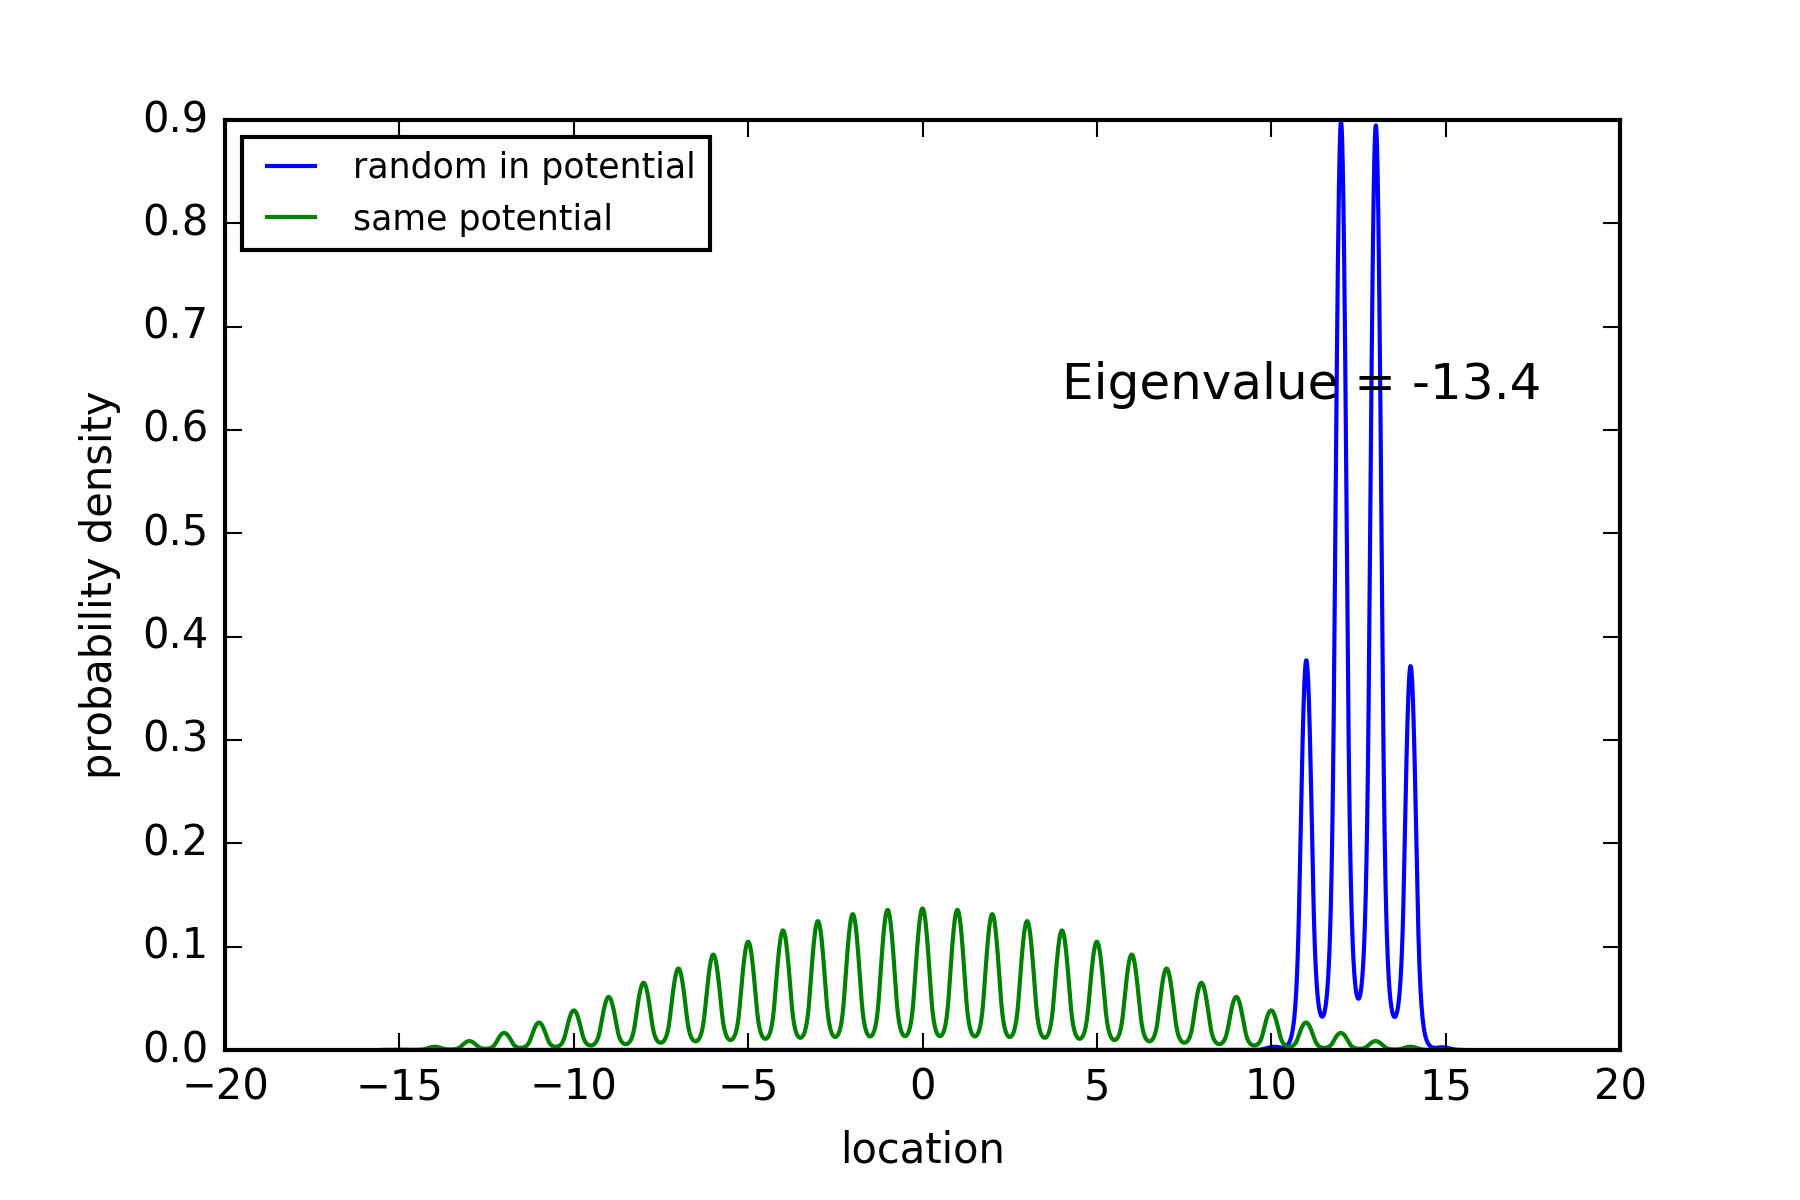
\includegraphics[width=1.1\linewidth]{RandomPotential2/10_0a_1th_Lowest_Rand0_4_0_5.png}
  \captionof{figure}{Lowest eigenvalue, $V_0l=10.0$, $w_1 = 0.4 $,$w_2 = 0.5$}
  \label{fig:randPoa10_1th_0.5_0.4}
\end{minipage}\qquad
\begin{minipage}{.45\textwidth}
  \centering
  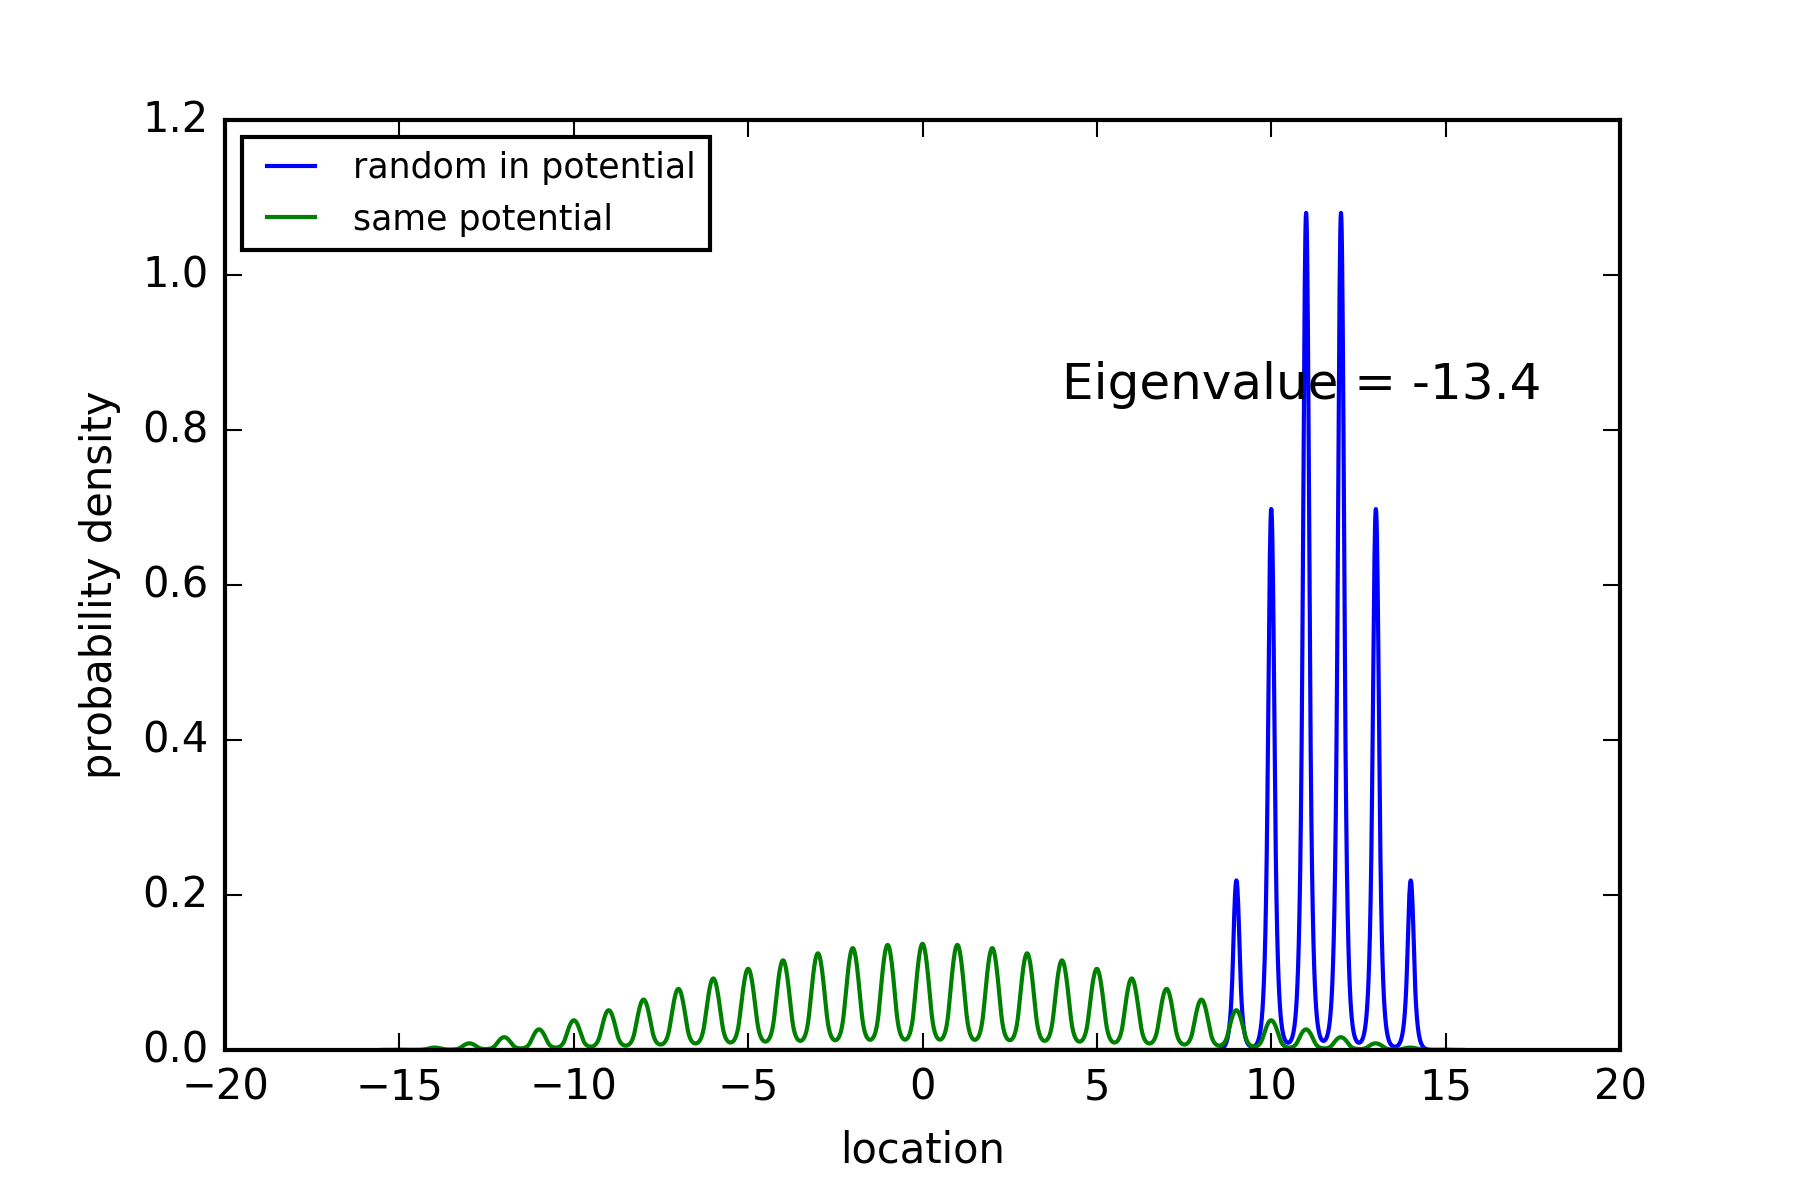
\includegraphics[width=1.1\linewidth]{RandomPotential2/10_0a_1th_Lowest_Rand0_2_0_5.png}
  \captionof{figure}{Lowest eigenvalue, $V_0l=10.0$, $w_1 = 0.2 $, $w_2 = 0.5 $}
  \label{fig:randPoa10_1th_0.5_0.2}
\end{minipage}
\end{figure}

%2nd lowest vl = 10.0
\begin{figure}[!htbh]
\centering
\begin{minipage}{.45\textwidth}
  \centering
  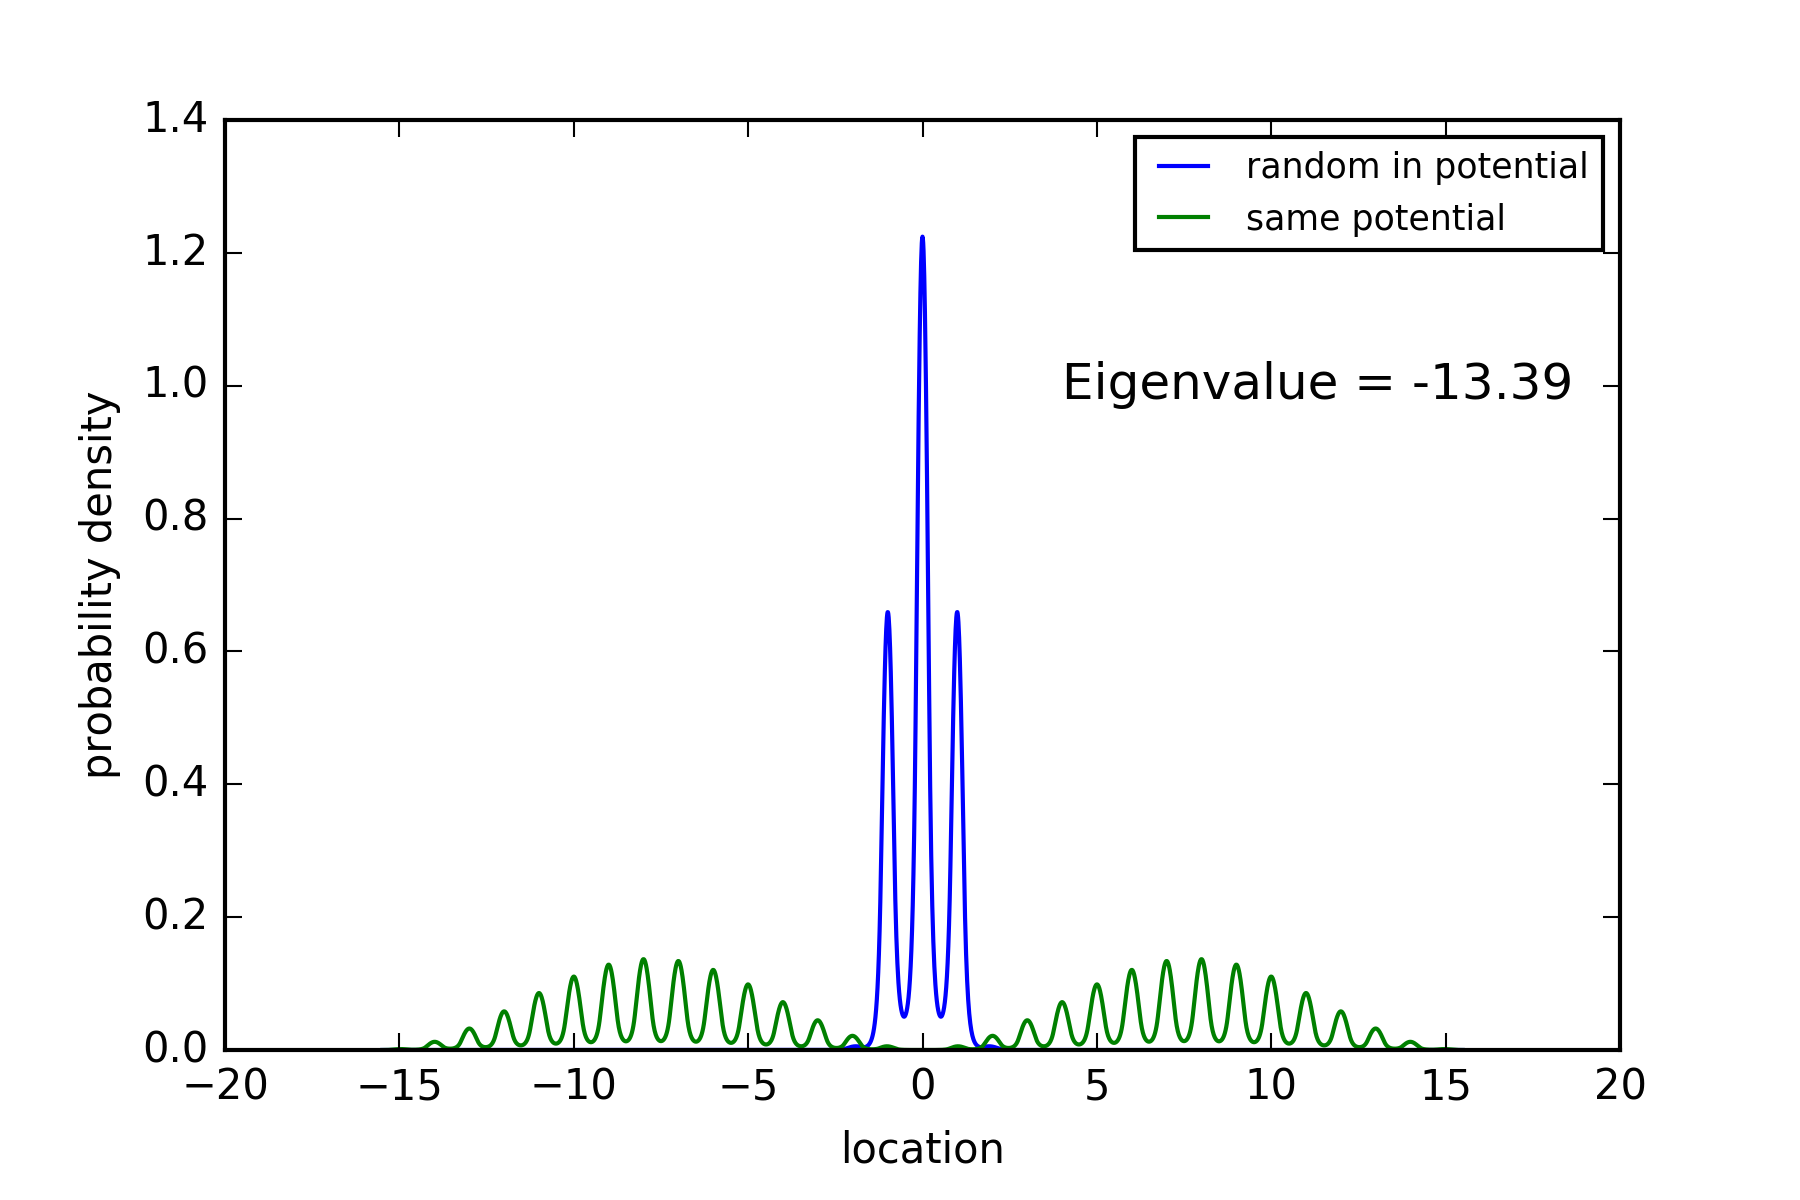
\includegraphics[width=1.1\linewidth]{RandomPotential2/10_0a_2th_Lowest_Rand0_4_0_5.png}
  \captionof{figure}{2nd Lowest eigenvalue, $V_0l =10.0$, $w_1 = 0.4 $,$w_2 = 0.5$}
  \label{fig:randPoa10_2th_0.5_0.4}
\end{minipage}\qquad
\begin{minipage}{.45\textwidth}
  \centering
  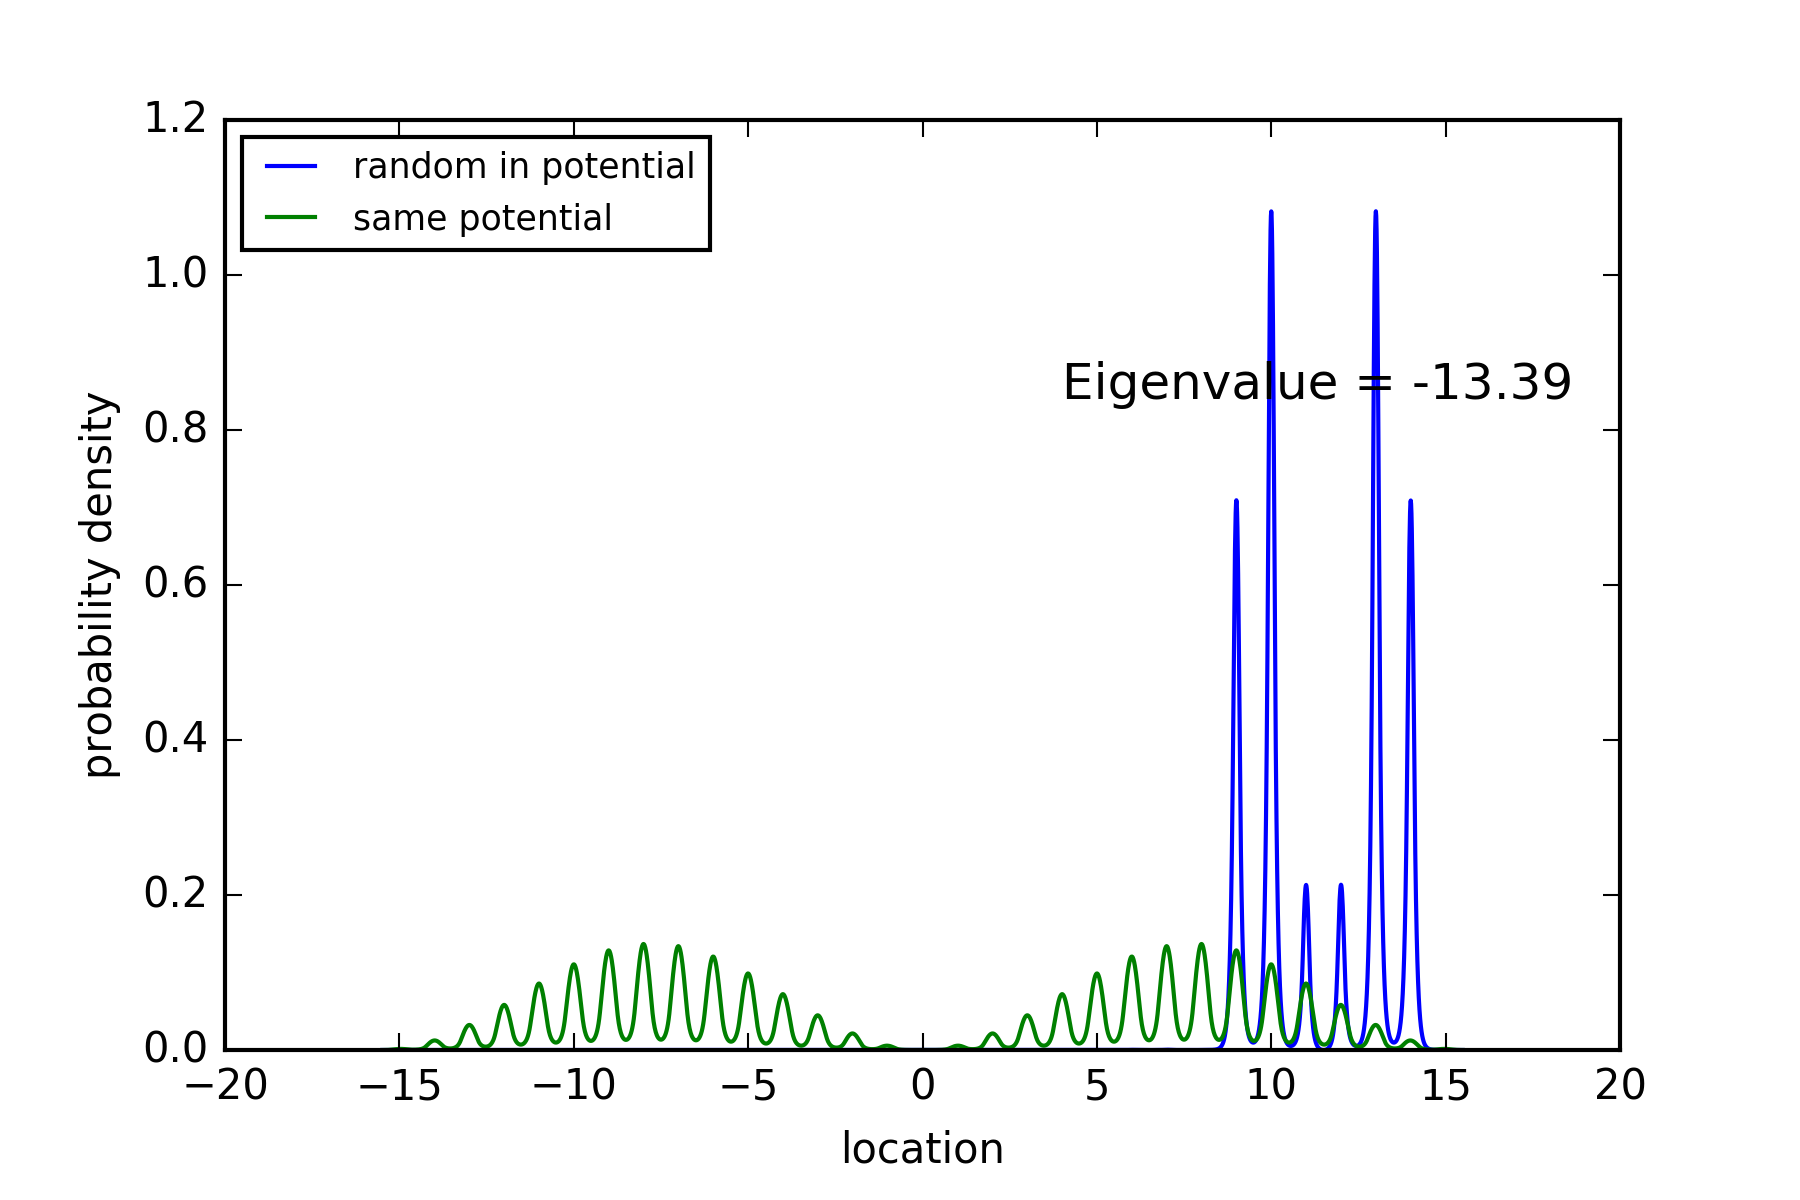
\includegraphics[width=1.1\linewidth]{RandomPotential2/10_0a_2th_Lowest_Rand0_2_0_5.png}
  \captionof{figure}{2nd Lowest eigenvalue, $V_0l=10.0$,$w_1 = 0.2 $, $w_2 = 0.5 $}
  \label{fig:randPoa10_2th_0.5_0.2}
\end{minipage}
\end{figure}


\newpage
\subsection{Localization caused by floating point precision}
This is another interesting situation where we see the localization property of disordered system caused by floating point precision and carelessly designed algorithm for determining the potential. 
Due to the binary representation in computer, most decimal cannot be represented precisely \cite{FloatingPrecision}. That means a decimal number, e.g. 0.1, may be represented in the machine as 0.09999999999999. 
When determining the potential, we iterate through the mesh points to see if it is in the closed neighborhood of some atom sites with radius of half of the well width. The problem occurs when the mesh point falls exactly on the boundary of the neighborhood because our original method didn't take the precision into consideration so that a mesh point at the boundary might be 0.00000000001 away from the boundary and not considered at a point with non-zero potential.
Our new method of determining the potential at each mesh points take the precision into consideration such that any mesh point on the boundary is correctly assigned with a potential value without any exception due to floating point precision.

The following first three figures are the eigenstates for a system with the old way of determining the potential, and the rest are that with the new way of determining the potential. 

%old 
\begin{figure}[!htbh]
\centering
\begin{minipage}{.45\textwidth}
  \centering
  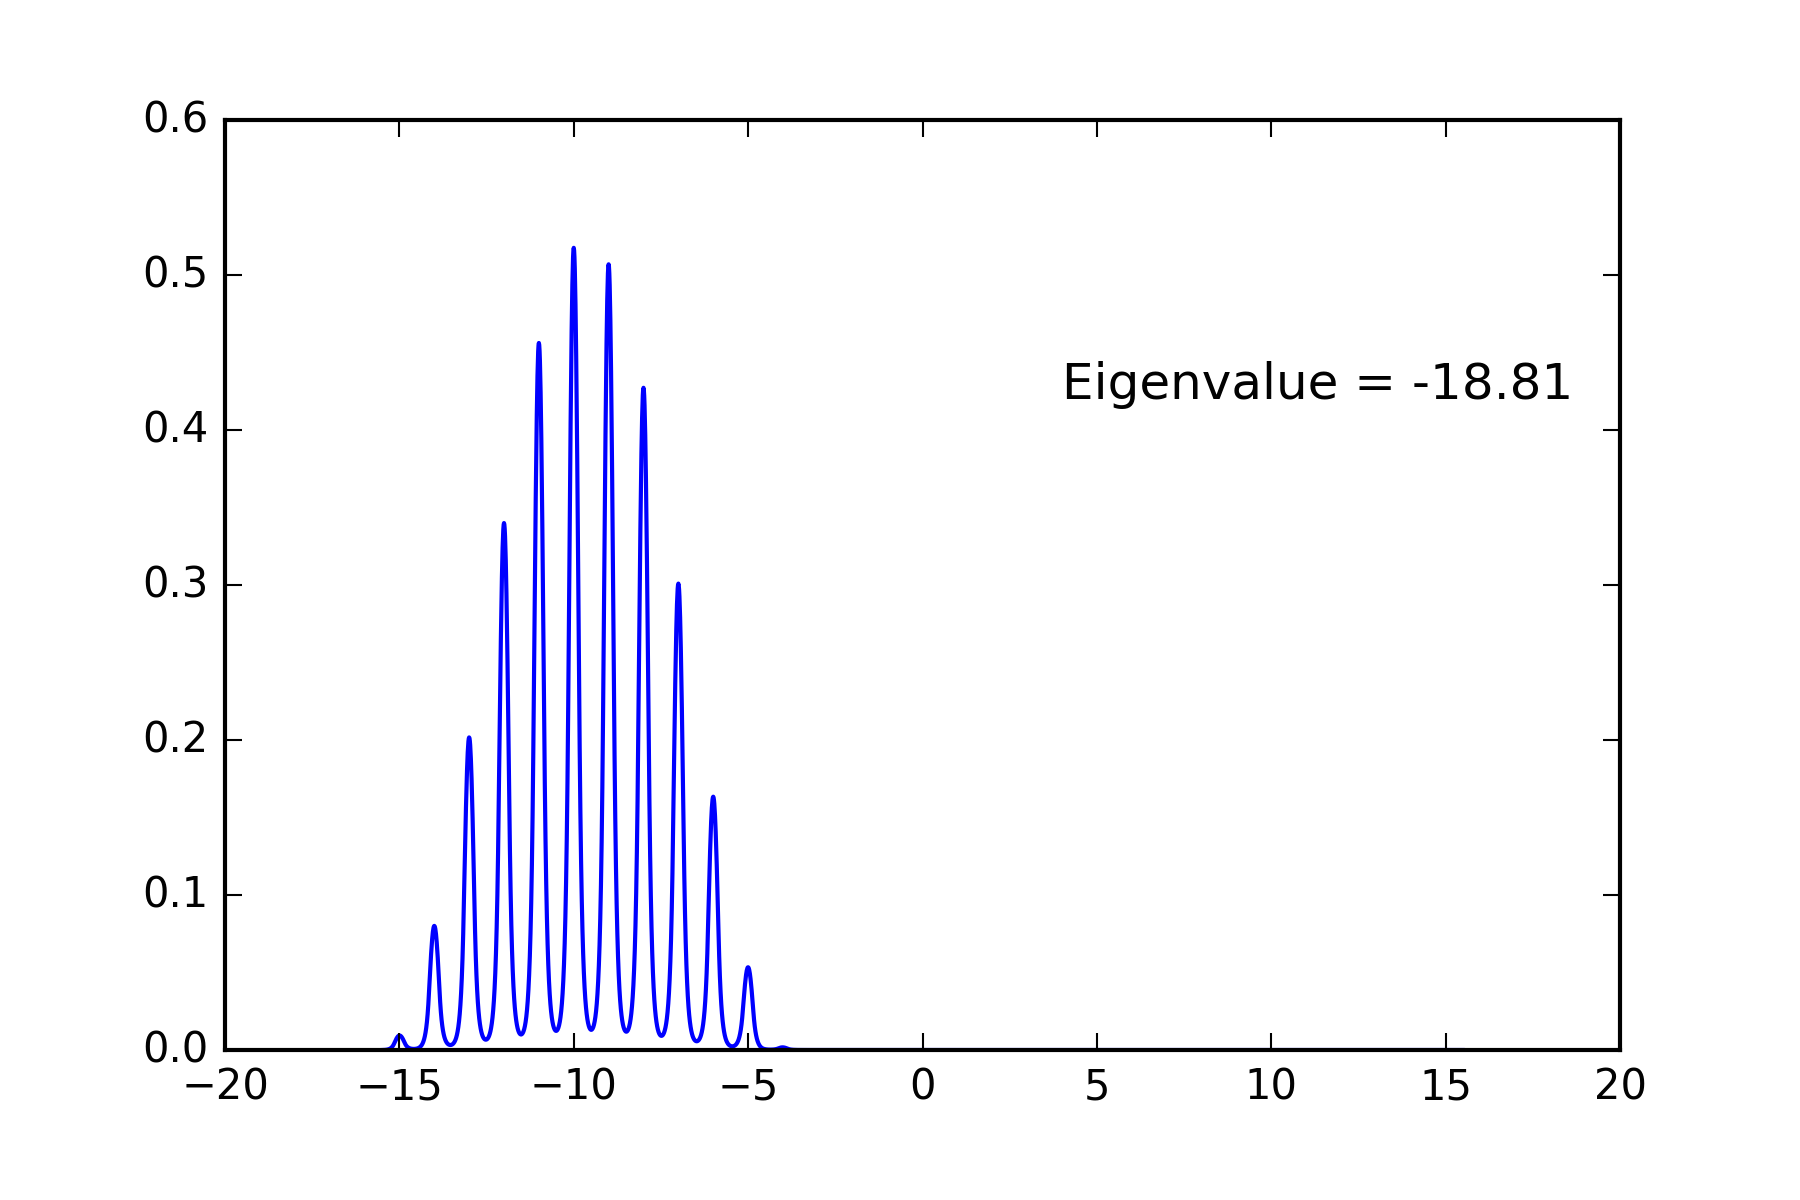
\includegraphics[width=1.1\linewidth]{floatingPrecision/oldPot100discrete_1th_Lowest0_3.png}
  \captionof{figure}{Old potential, $V_0l =10.0$, $l=0.4 $, discretization accuracy $= 0.01 $}
  \label{fig:oldPo_0.4}
\end{minipage}\qquad
\begin{minipage}{.45\textwidth}
  \centering
  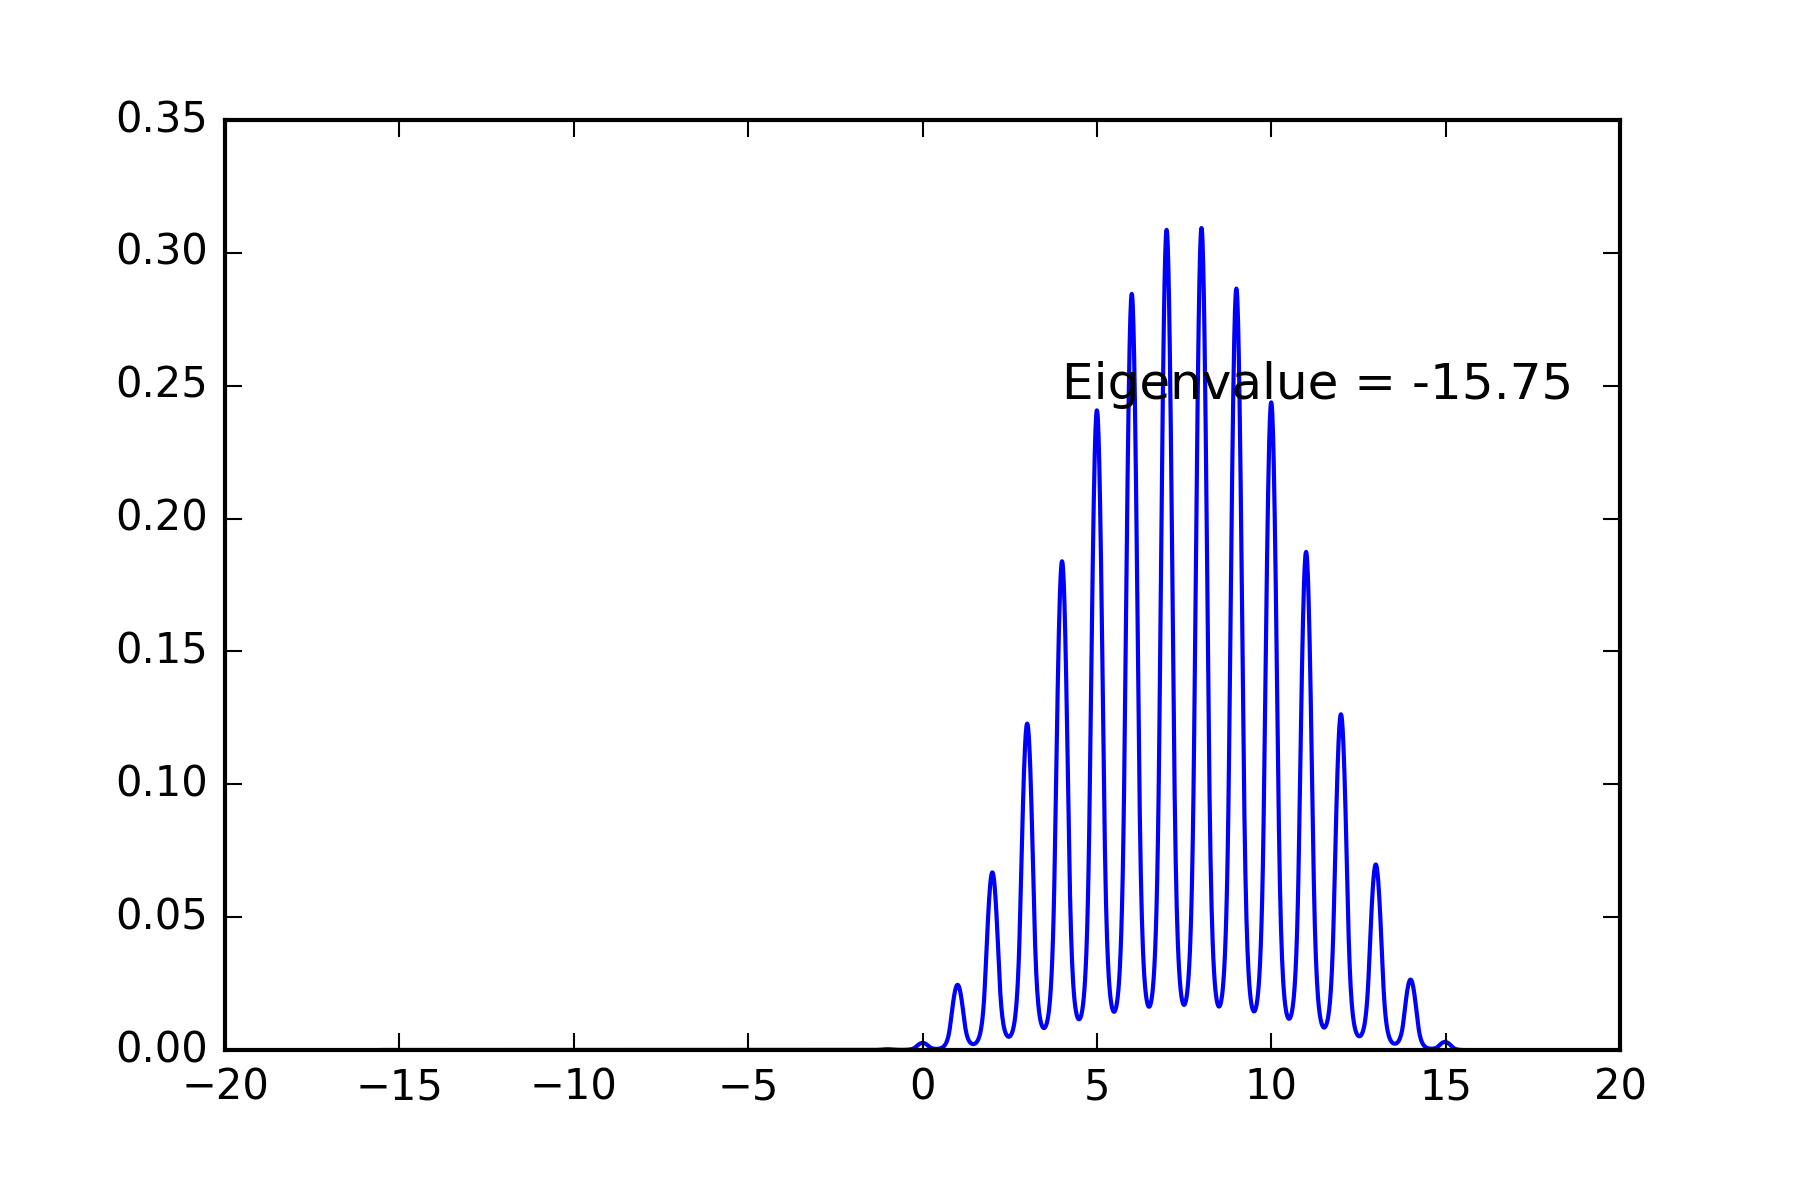
\includegraphics[width=1.1\linewidth]{floatingPrecision/oldPot100discrete_1th_Lowest0_4.png}
  \captionof{figure}{Old potential, $V_0l=10.0$, $l = 0.3 $,discretization accuracy $= 0.01$}
  \label{fig:oldPo_0.3}
\end{minipage}
\end{figure}

%old 
\begin{figure}[!htbh]
\centering
\begin{minipage}{.45\textwidth}
  \centering
  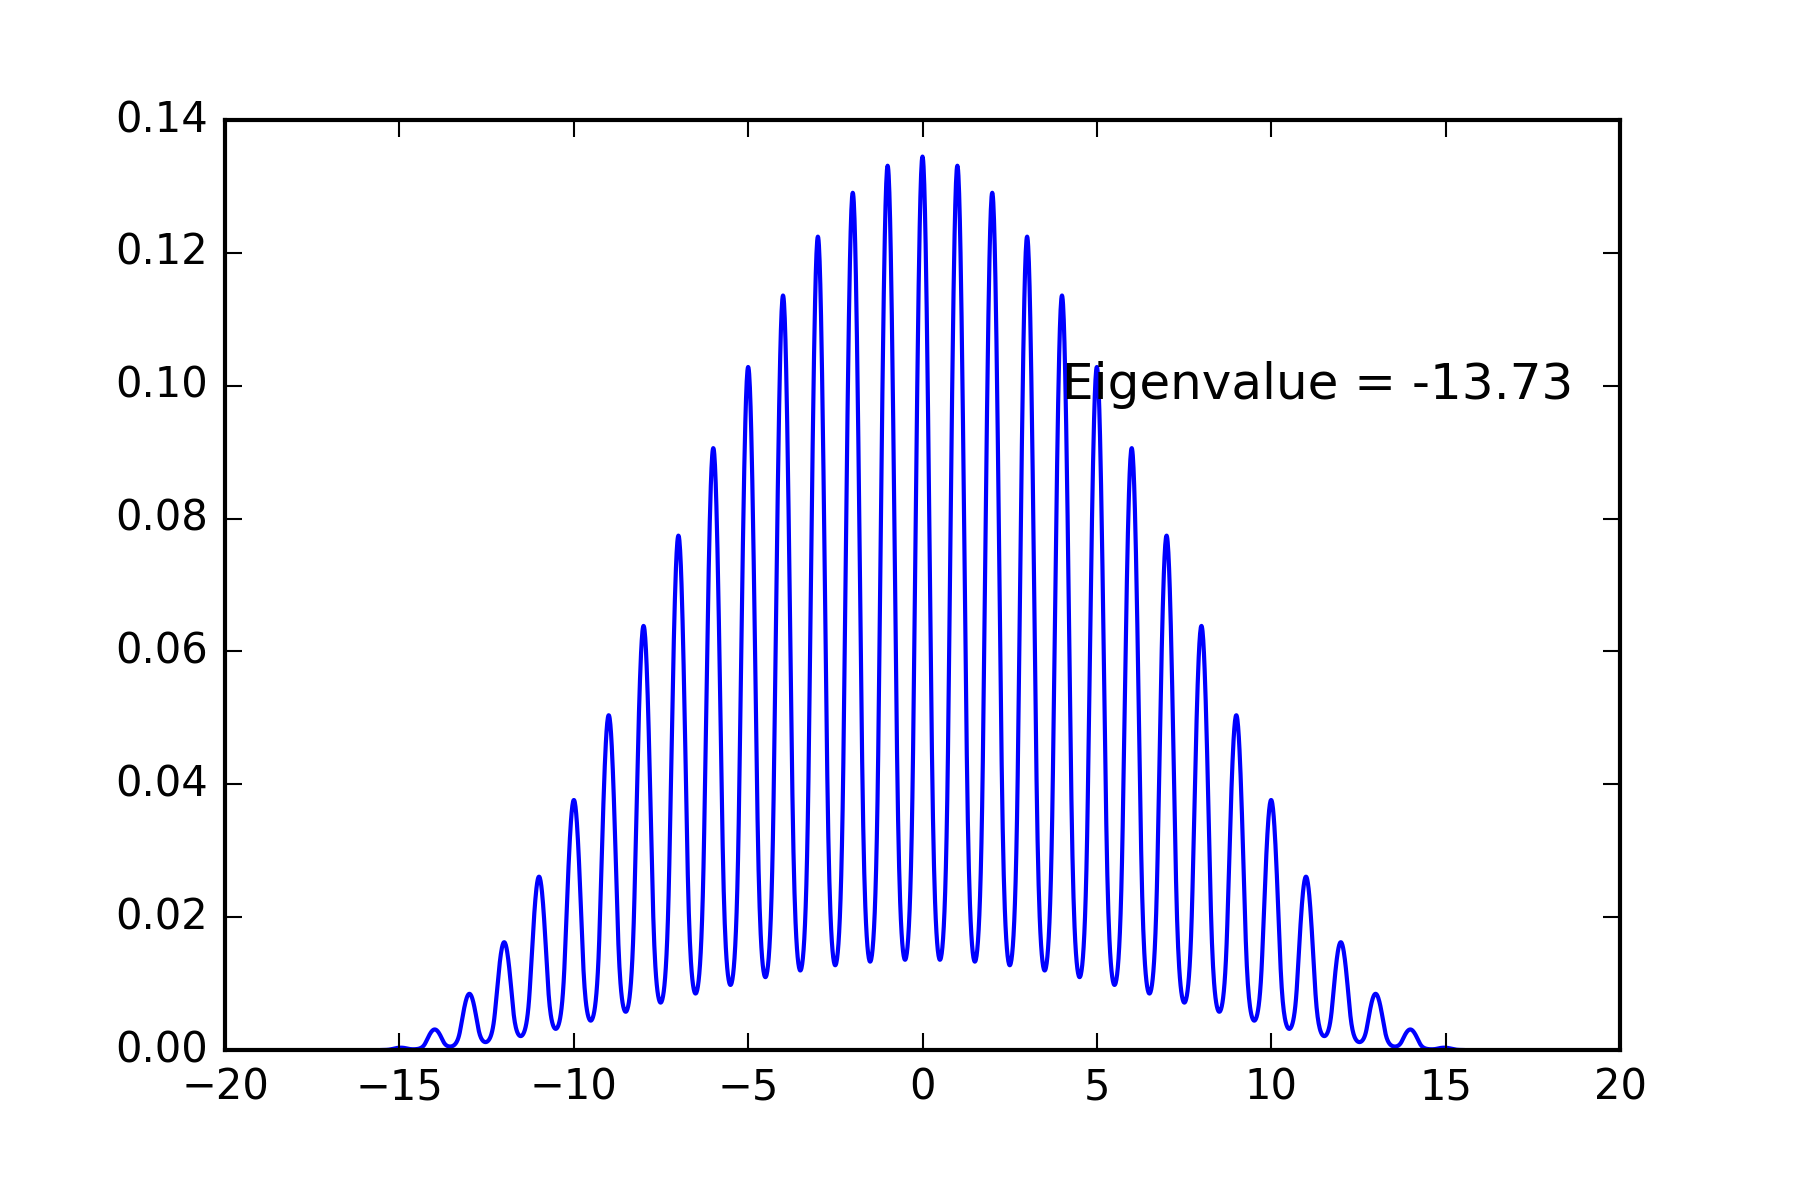
\includegraphics[width=1.1\linewidth]{floatingPrecision/oldPot100discrete_1th_Lowest0_5.png}
  \captionof{figure}{Old potential, $V_0l=10.0$, $l = 0.5 $,discretization accuracy $= 0.01 $}
  \label{fig:oldPo_0.5}
\end{minipage}\qquad
%new
\begin{minipage}{.45\textwidth}
  \centering
  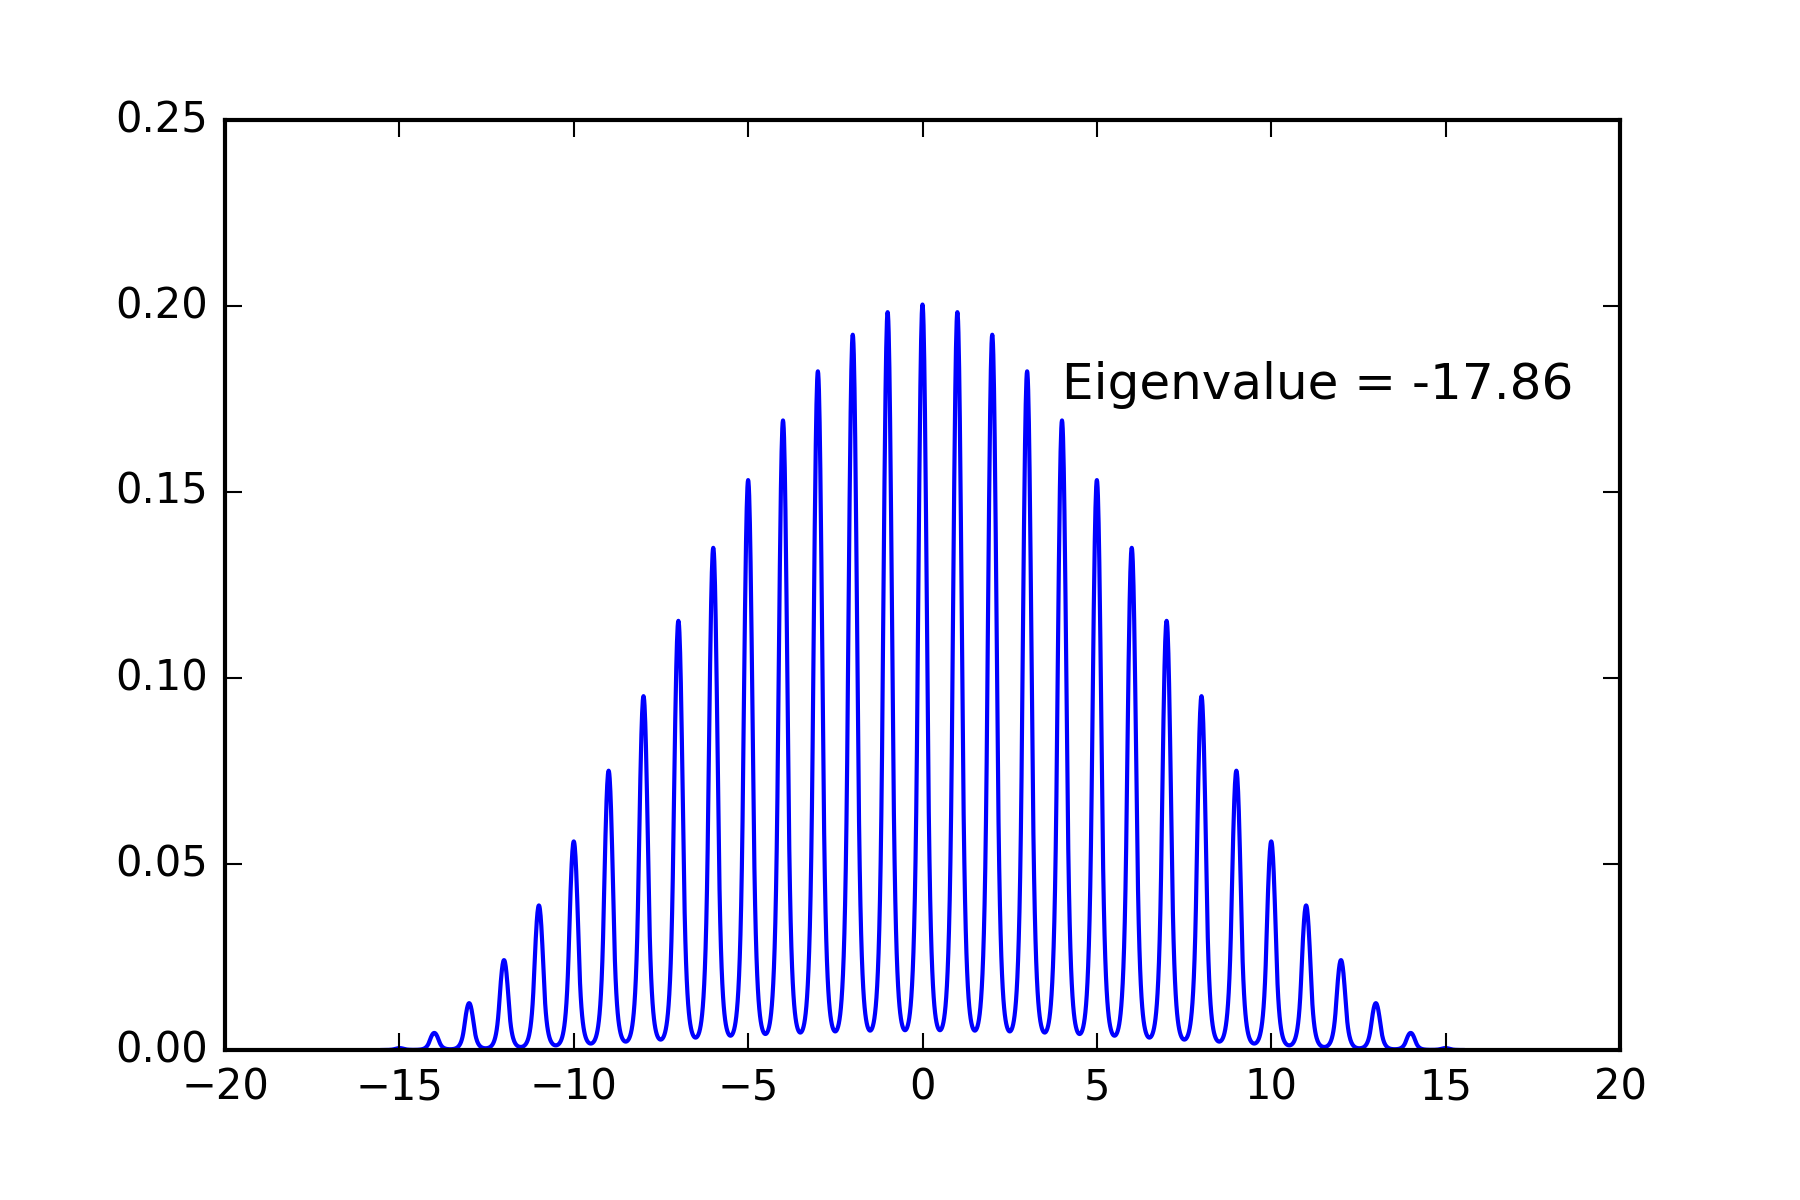
\includegraphics[width=1.1\linewidth]{floatingPrecision/newPot100discrete_1th_Lowest0_3.png}
  \captionof{figure}{New potential,  $V_0l=10.0$, $l = 0.3 $,discretization accuracy $= 0.01 $}
  \label{fig:newPo_0.3}
\end{minipage}
\end{figure}

%new
\begin{figure}[!htbh]
\centering
\begin{minipage}{.45\textwidth}
  \centering
  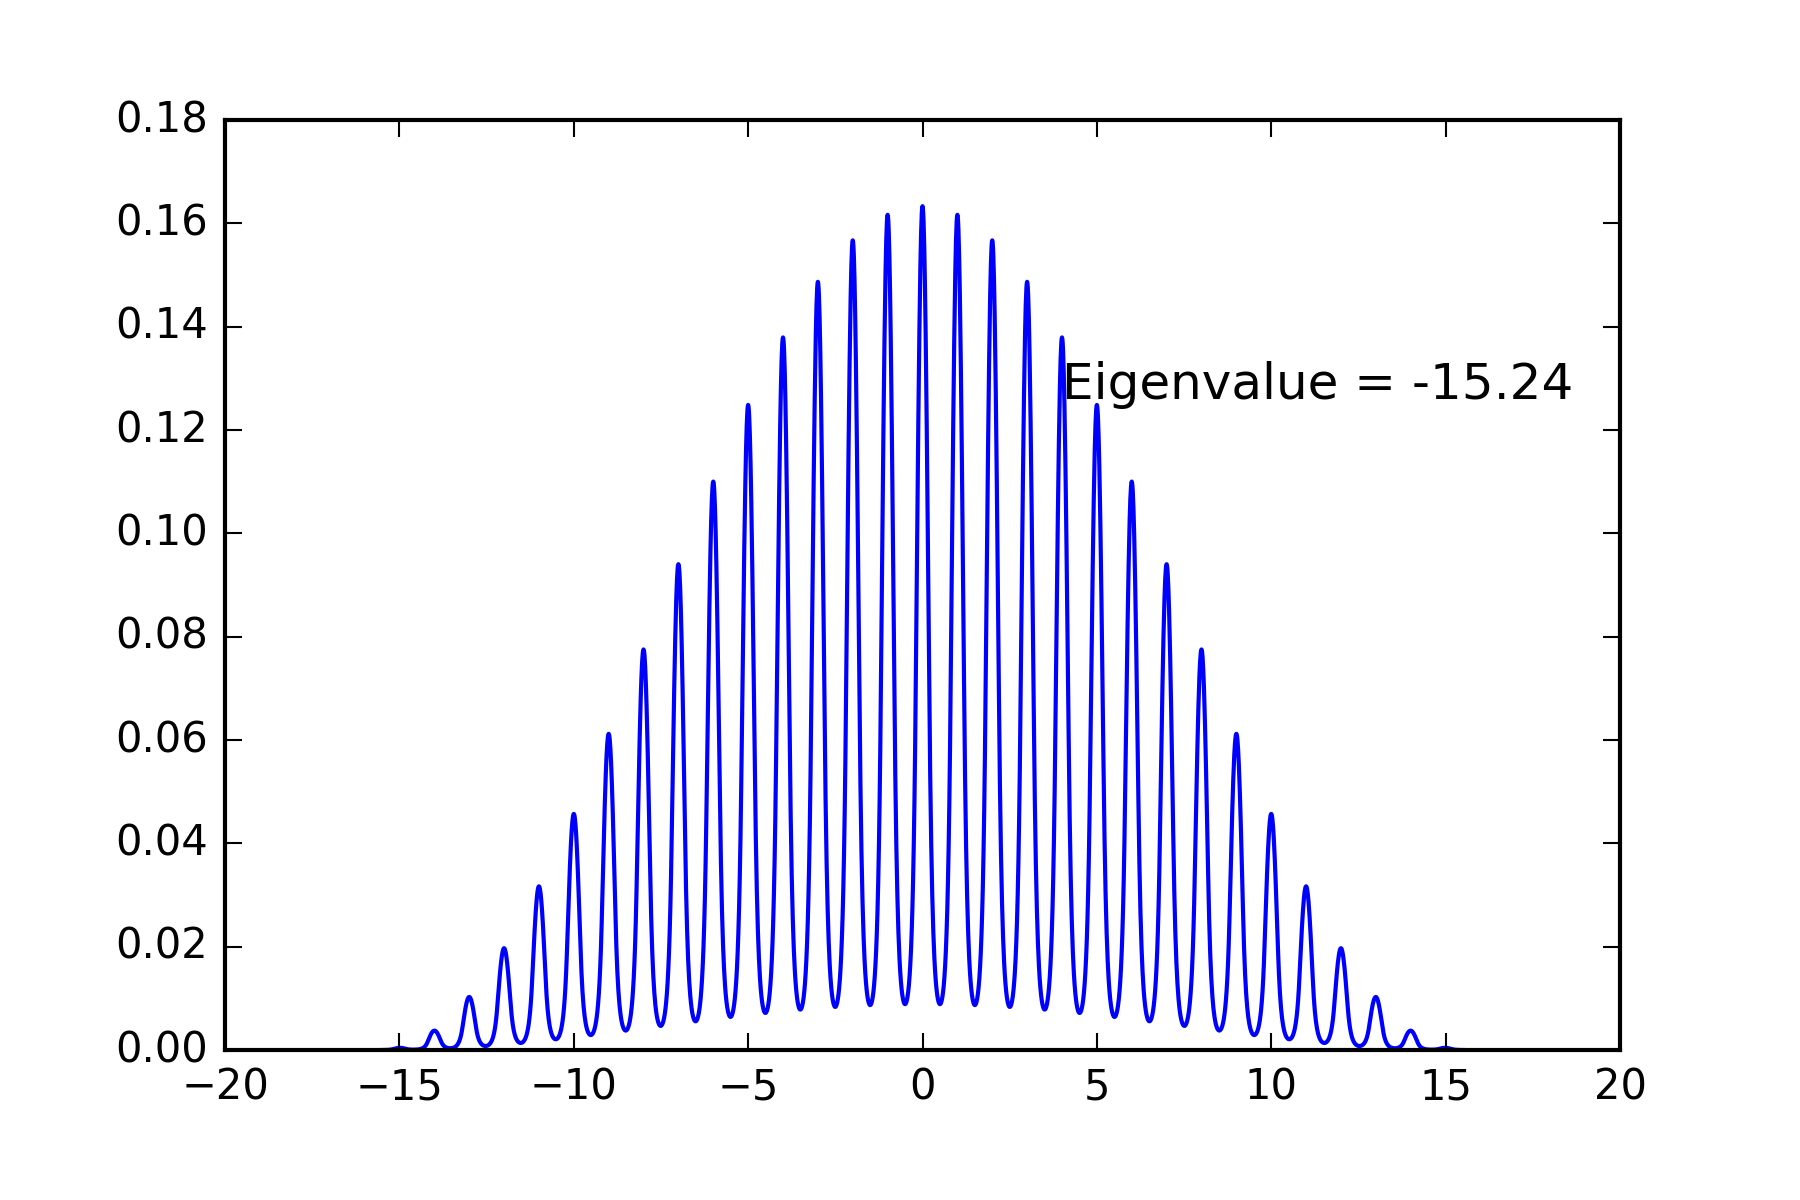
\includegraphics[width=1.1\linewidth]{floatingPrecision/newPot100discrete_1th_Lowest0_4.png}
  \captionof{figure}{New potential,  $V_0l=10.0$, $l = 0.4 $, discretization accuracy $= 0.01 $}
  \label{fig:newPo_0.4}
\end{minipage}\qquad
\begin{minipage}{.45\textwidth}
  \centering
  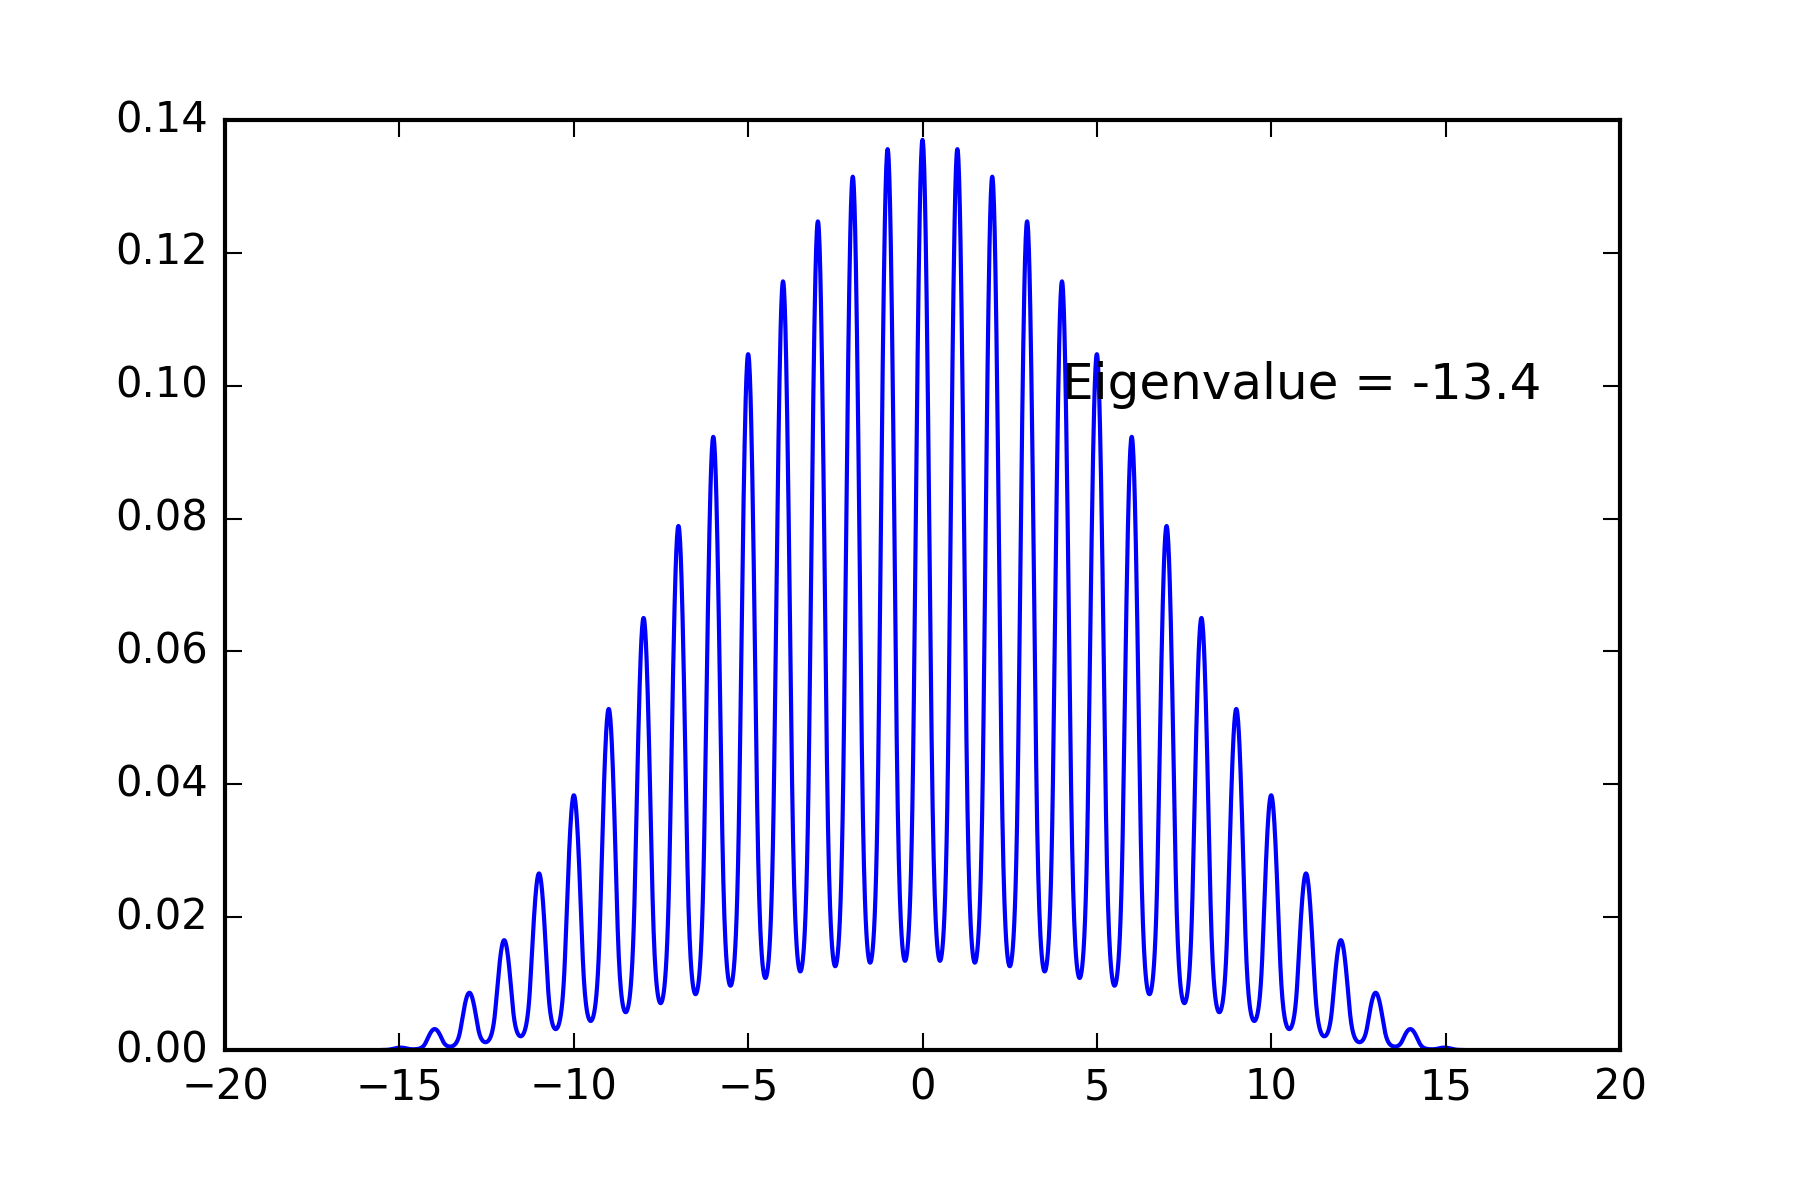
\includegraphics[width=1.1\linewidth]{floatingPrecision/newPot100discrete_1th_Lowest0_5.png}
  \captionof{figure}{New potential, $V_0l=10.0$, $l = 0.5 $, discretization accuracy $= 0.01 $}
  \label{fig:newPo_0.5}
\end{minipage}
\end{figure}

%A measure for degree of localization
\newpage
\subsection{A measure for degree of localization}
We try a way of defining degree of localization for eigenstates using standard deviation, which can be computed from the probability density function.
The advantage of defining such a measure is to allow us to compare localization quantitatively under different conditions. With this measure, we can also plot the standard deviations at different energy levels for two systems, namely a regular system, and a disordered system, in order to compare localization at different energy levels. 
Note that for the disordered system, we handle randomness by computing the standard deviations for 101 samples and taking an average.

The parameters for the regular and disordered systems are listed below in the table (Note that each parameter is defined in previous sections) followed by the corresponding figures for standard deviations against energy levels. 


\newpage
\begin{table}[]
\centering
\begin{tabular}{|l|l|l|l|l|}
\hline
	 & number of atoms  &$V_0l$& atomic spacings & probabilities   \\ \hline
Regular system&31& 10.0  & {1.0}  & {1} \\ \hline
Disordered System No.1 &31 &10.0   & {1.1,1.0}  & {0.5,0.5}    \\ \hline
Disordered System No.2 &31 &10.0   & {1.5,1.0}  & {0.5,0.5}    \\ \hline
Disordered System No.3 &31 &30.0   & {1.1,1.0}  & {0.5,0.5}    \\ \hline
Disordered System No.4 &31 &30.0   & {1.1,1.0}  & {0.5,0.5}    \\ \hline
\end{tabular}
\centering
\end{table}



%start figure
\begin{figure}[!htbh]
\centering
\begin{minipage}{.45\textwidth}
  \centering
  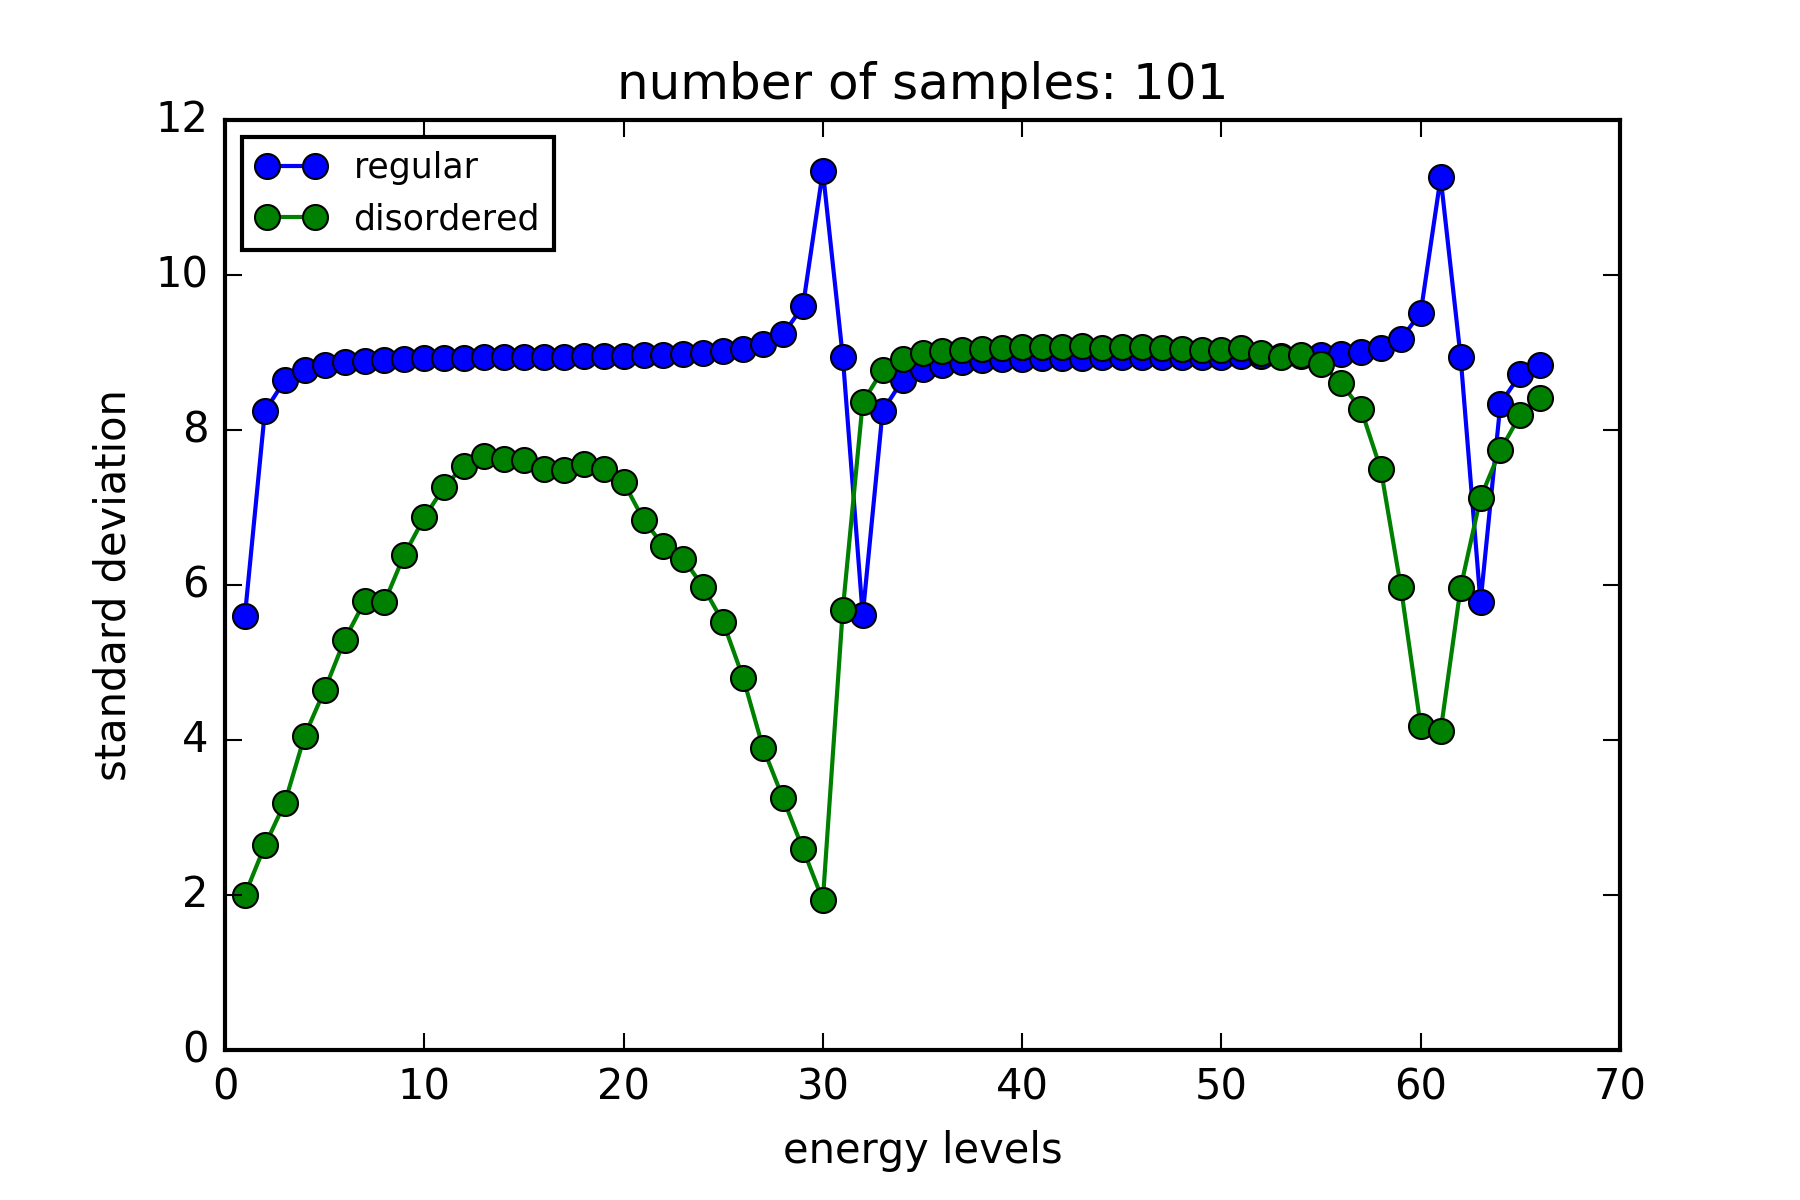
\includegraphics[width=1.1\linewidth]{standardDeviation/N_31_100a10_0_1_1_p_0_5.png}
  \captionof{figure}{Localization against energy levels, comparison between Regular System and Disordered System No.1}
  \label{fig:disordered sys num 1}
\end{minipage}\qquad
\begin{minipage}{.45\textwidth}
  \centering
  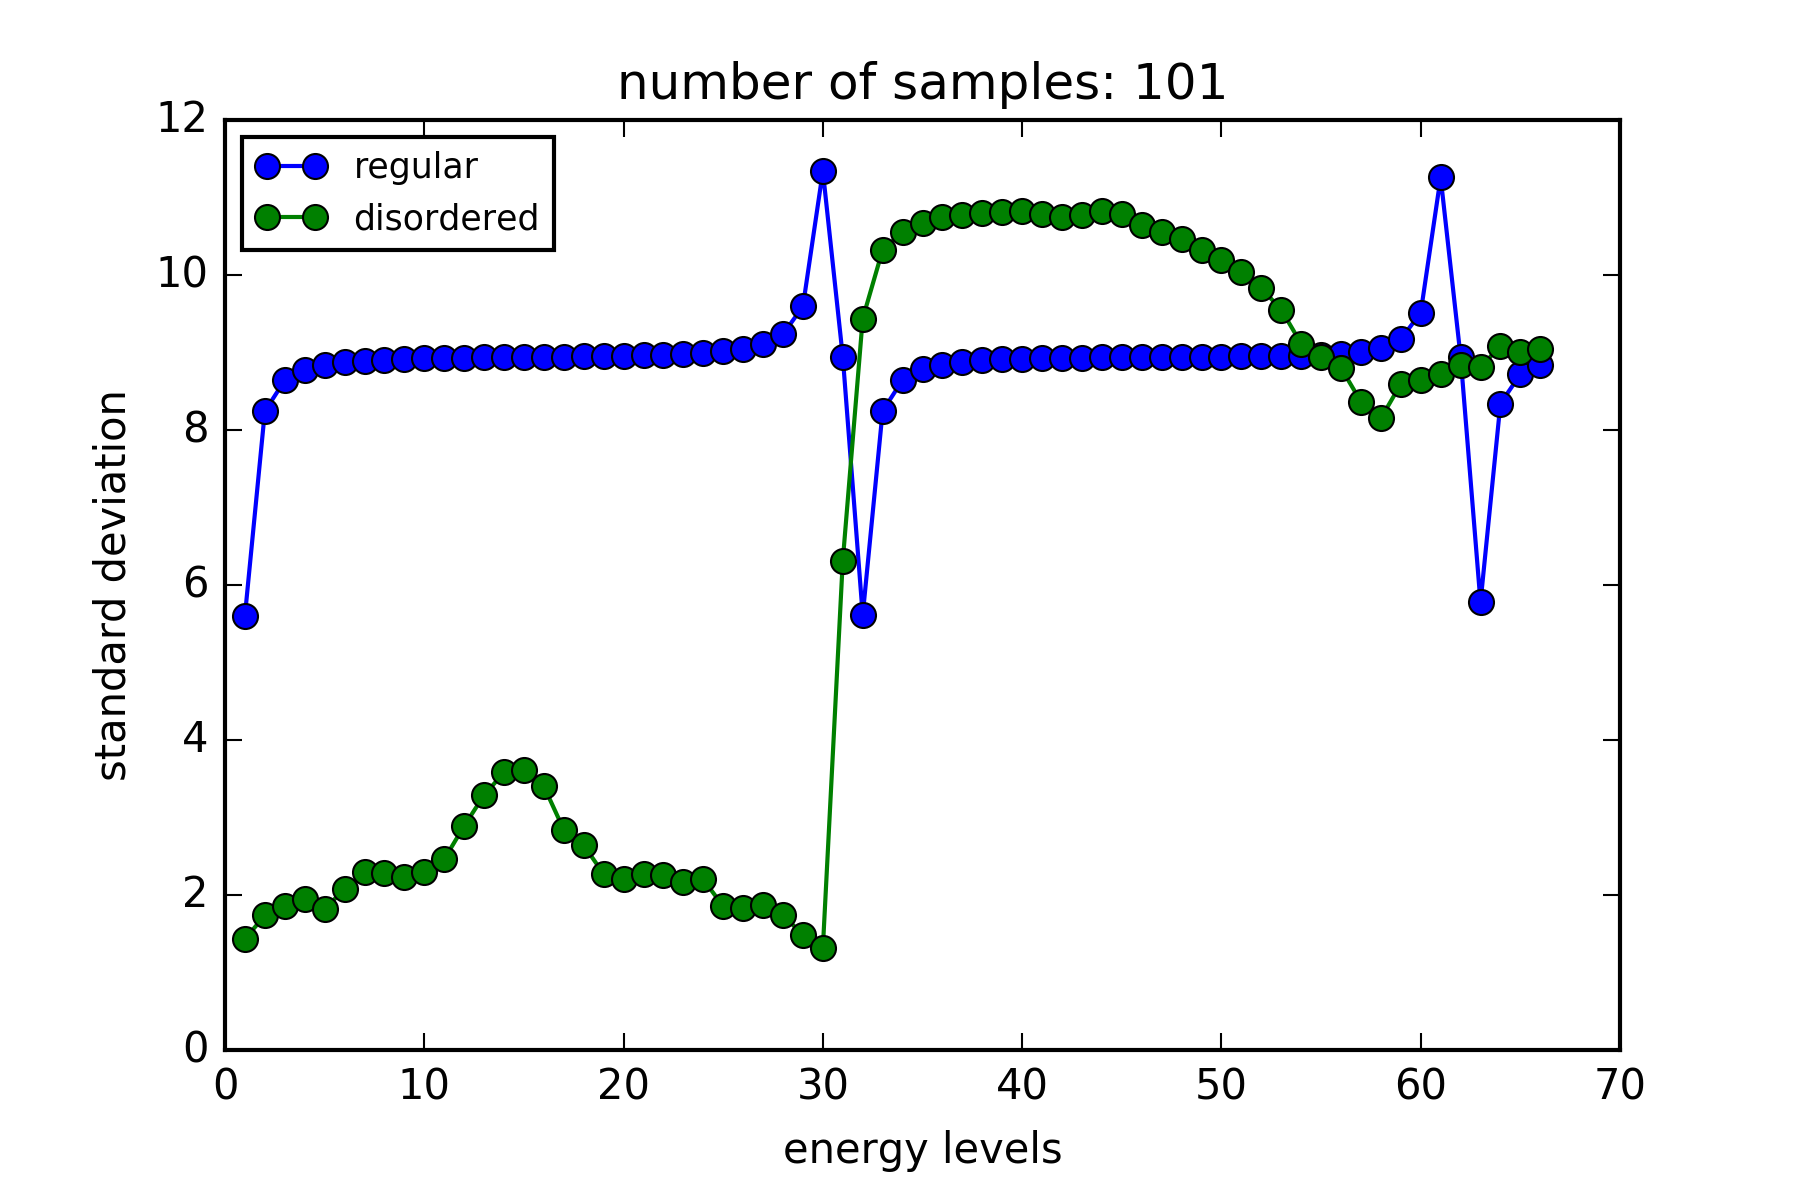
\includegraphics[width=1.1\linewidth]{standardDeviation/N_31_100a10_0_1_5_p_0_5.png}
  \captionof{figure}{Localization against energy levels, comparison between Regular System and Disordered System No.2}
  \label{fig:disordered sys num 2}
\end{minipage}
\end{figure}

%a = 30 
\begin{figure}[!htbh]
\centering
\begin{minipage}{.45\textwidth}
  \centering
  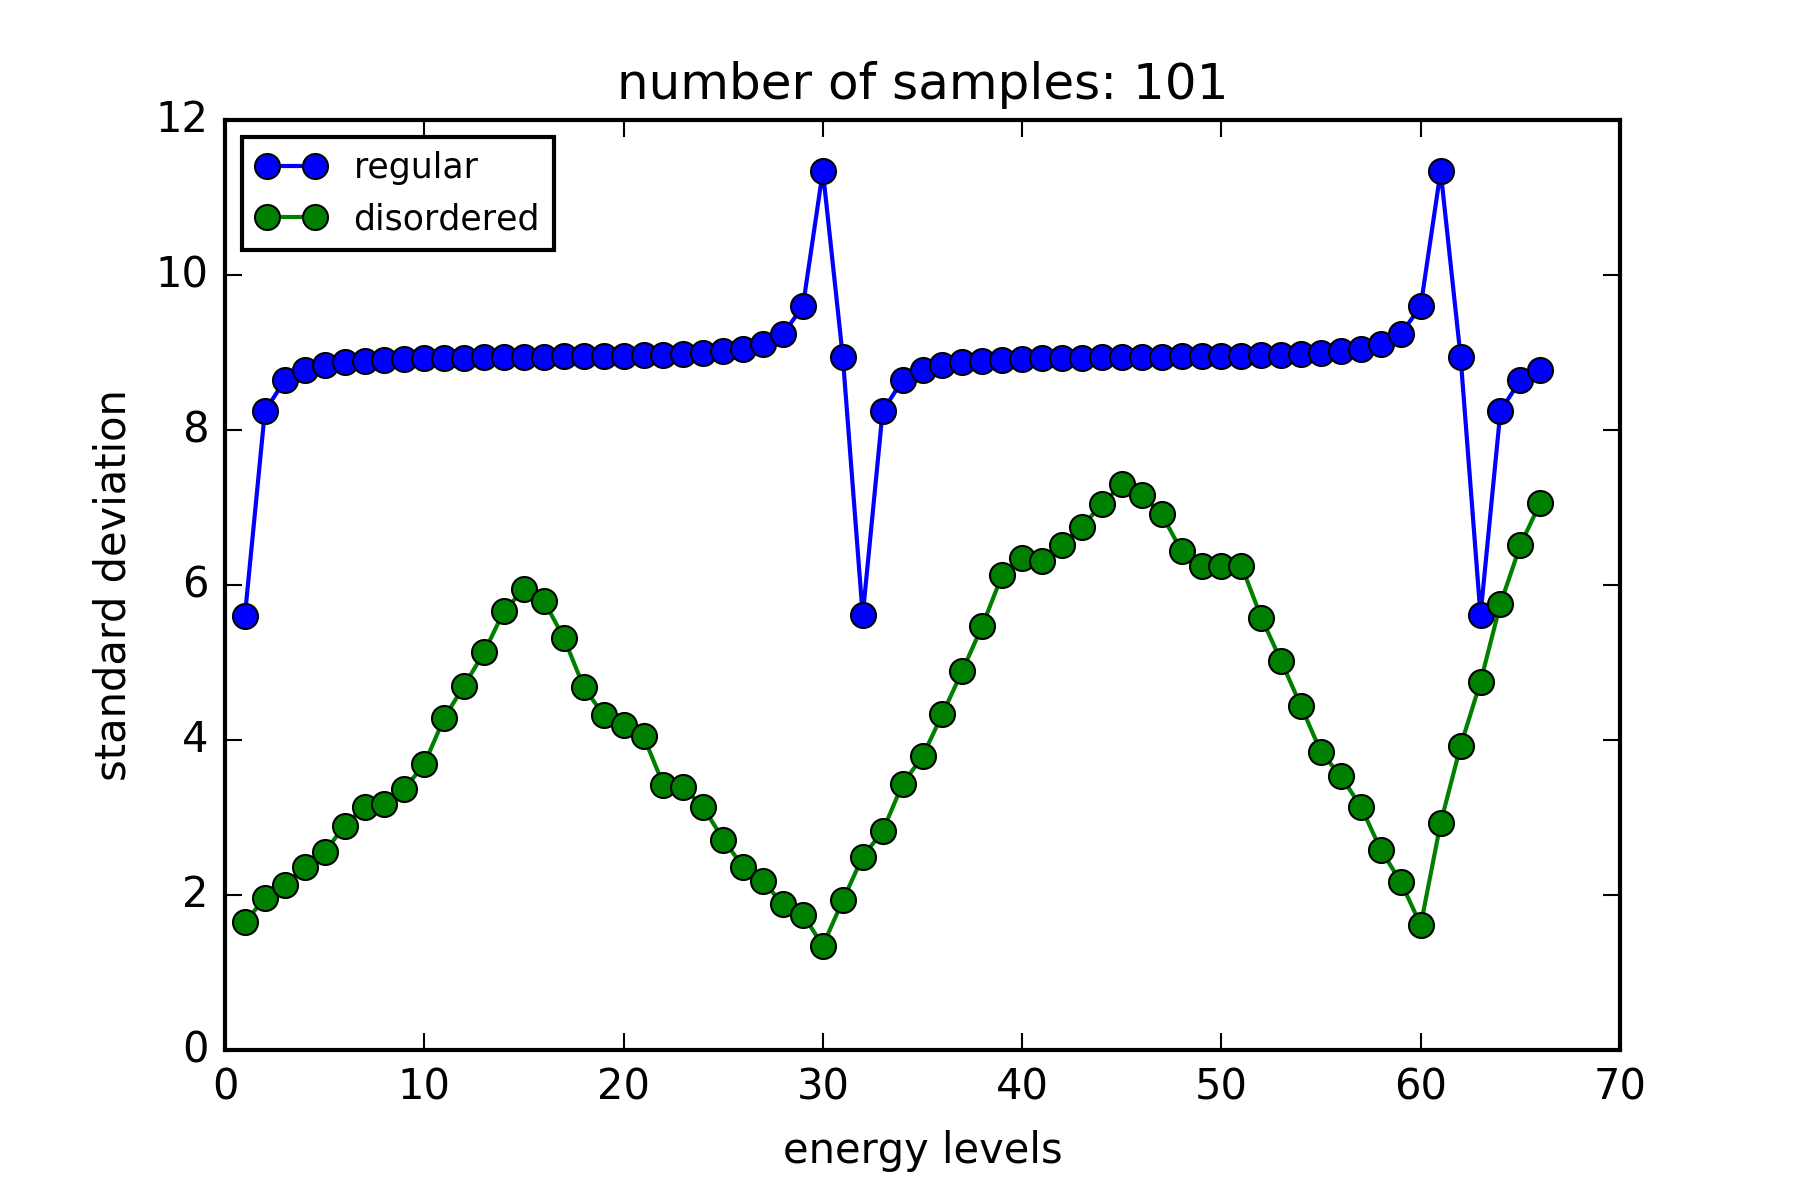
\includegraphics[width=1.1\linewidth]{standardDeviation/N_31_100a30_0_1_1_p_0_5.png}
  \captionof{figure}{Localization against energy levels, comparison between Regular System and Disordered System No.3}
  \label{fig:disordered sys num 3}
\end{minipage}\qquad
\begin{minipage}{.45\textwidth}
  \centering
  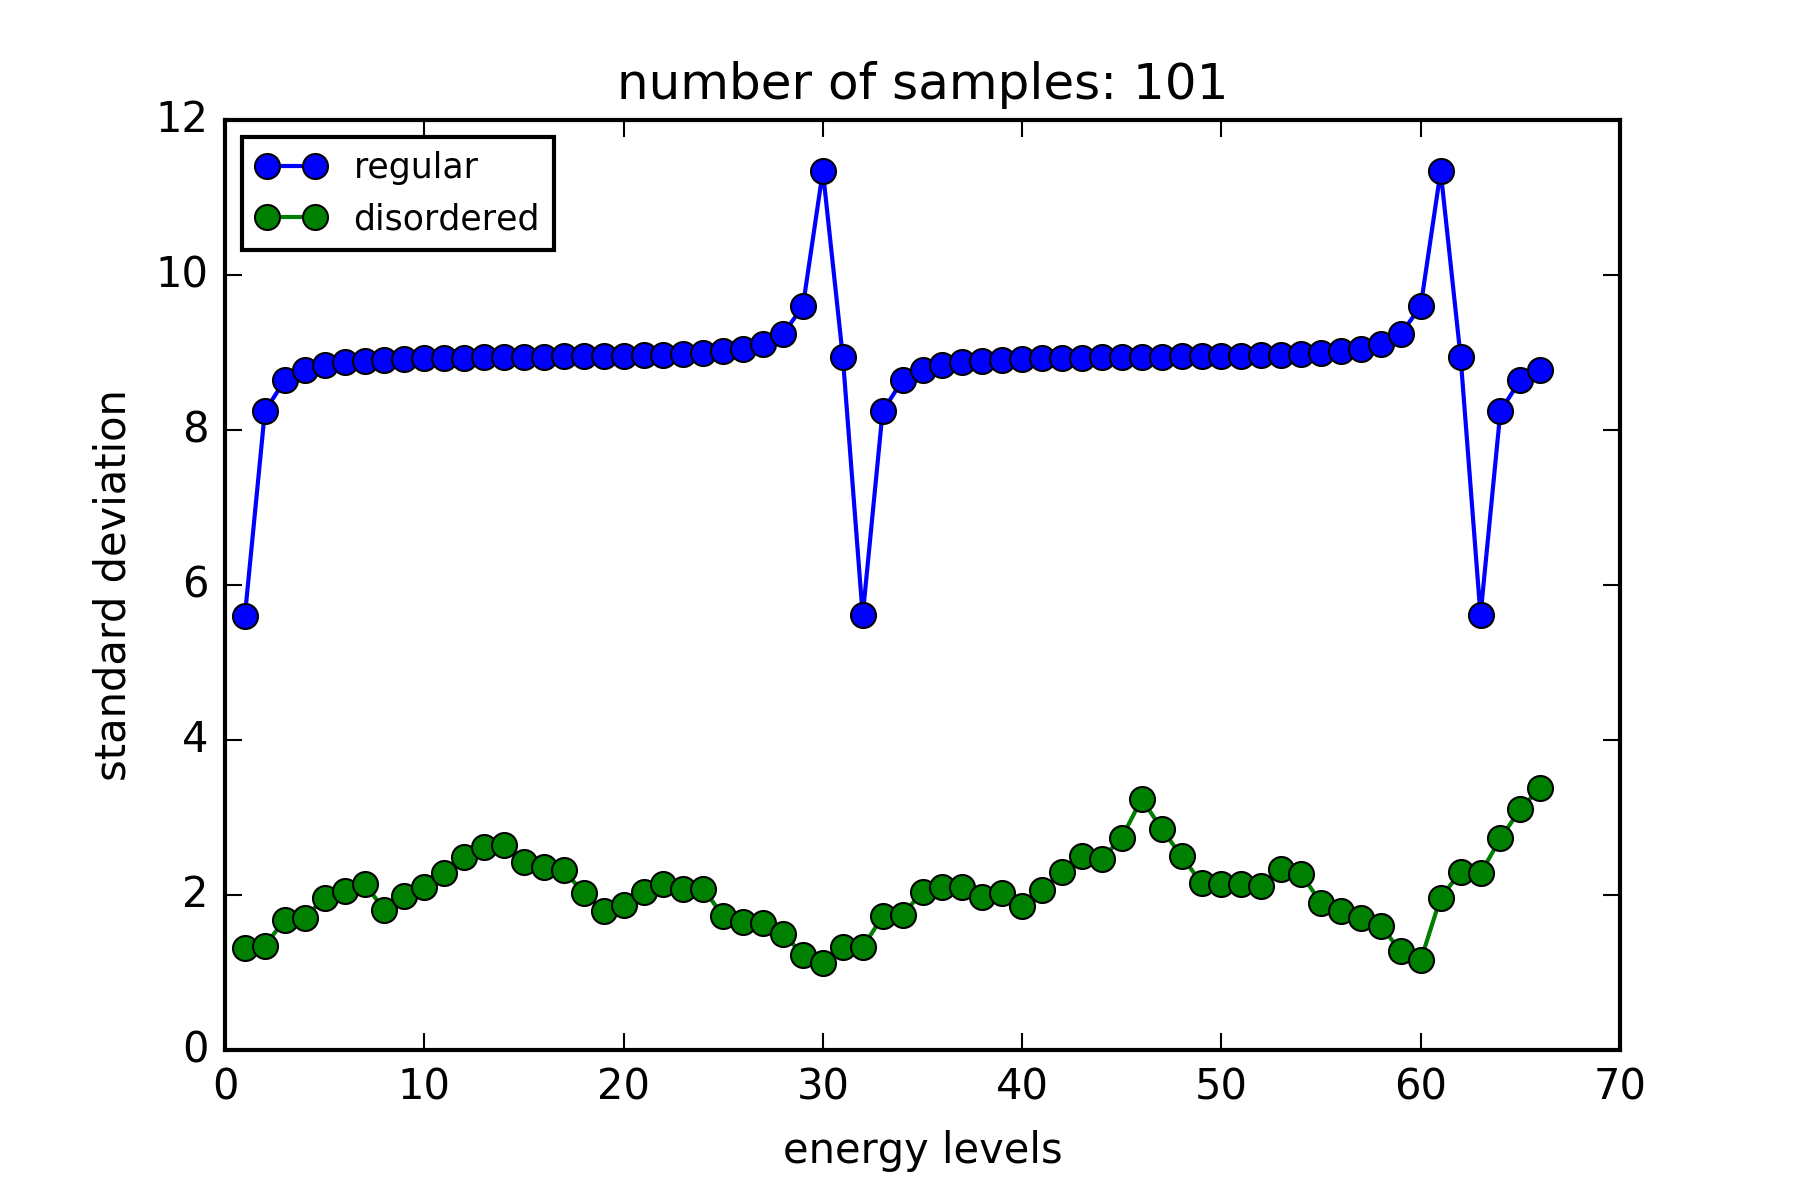
\includegraphics[width=1.1\linewidth]{standardDeviation/N_31_100a30_0_1_5_p_0_5.png}
  \captionof{figure}{Localization against energy levels, comparison between Regular System and Disordered System No.4}
  \label{fig:disordered sys num 4}
\end{minipage}
\end{figure}
%end figure

The following are figures for disordered systems with randomness in potential, in which we fix the square potential area and pick the well width from two values$\{w_1,w_2\}$ with probability $\{0.5,0.5\}$. 
The table lists the parameters for the regular system and different disordered systems. 

\newpage
\begin{table}[]
\centering
\begin{tabular}{|l|l|l|l|l|}
\hline
	 & number of atoms  &$V_0l$& well width $\{w_1,w_2\}$ & probabilities   \\ \hline
Regular system&31& 10.0  & {0.5}  & {1} \\ \hline
Disordered System No.5 &31 &10.0   & {0.4,0.5}  & {0.5,0.5}    \\ \hline
Disordered System No.6 &31 &10.0   & {0.2,0.5}  & {0.5,0.5}    \\ \hline
Disordered System No.7 &31 &30.0   & {0.4,0.5}  & {0.5,0.5}    \\ \hline
Disordered System No.8 &31 &30.0   & {0.2,0.5}  & {0.5,0.5}    \\ \hline
\end{tabular}
\centering
\end{table}

%randomness in potential 

%start figure
\begin{figure}[!htbh]
\centering
\begin{minipage}{.45\textwidth}
  \centering
  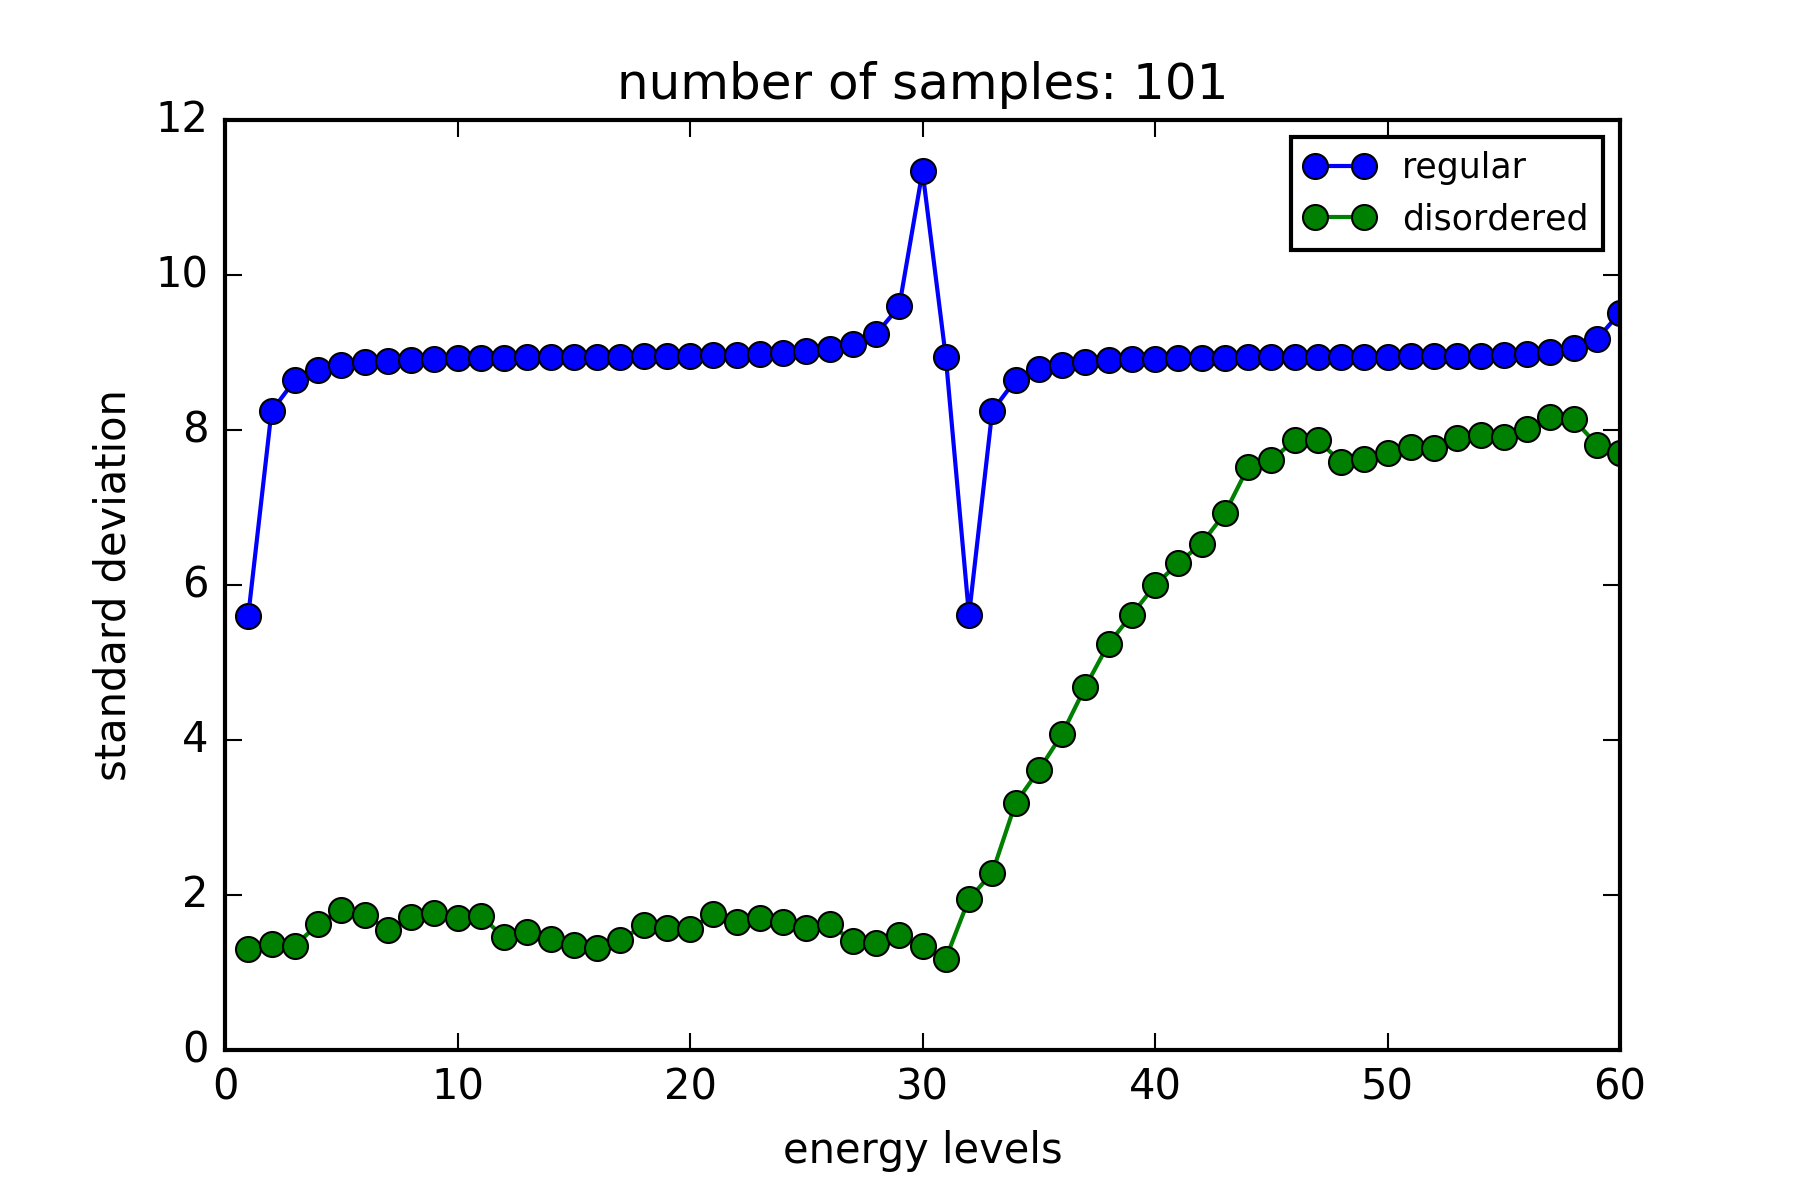
\includegraphics[width=1.1\linewidth]{standardDeviation/N_31_100a10_well0_4_p_0_5.png}
  \captionof{figure}{Localization against energy levels, comparison between Regular System and Disordered System No.5}
  \label{fig:disordered sys num 5}
\end{minipage}\qquad
\begin{minipage}{.45\textwidth}
  \centering
  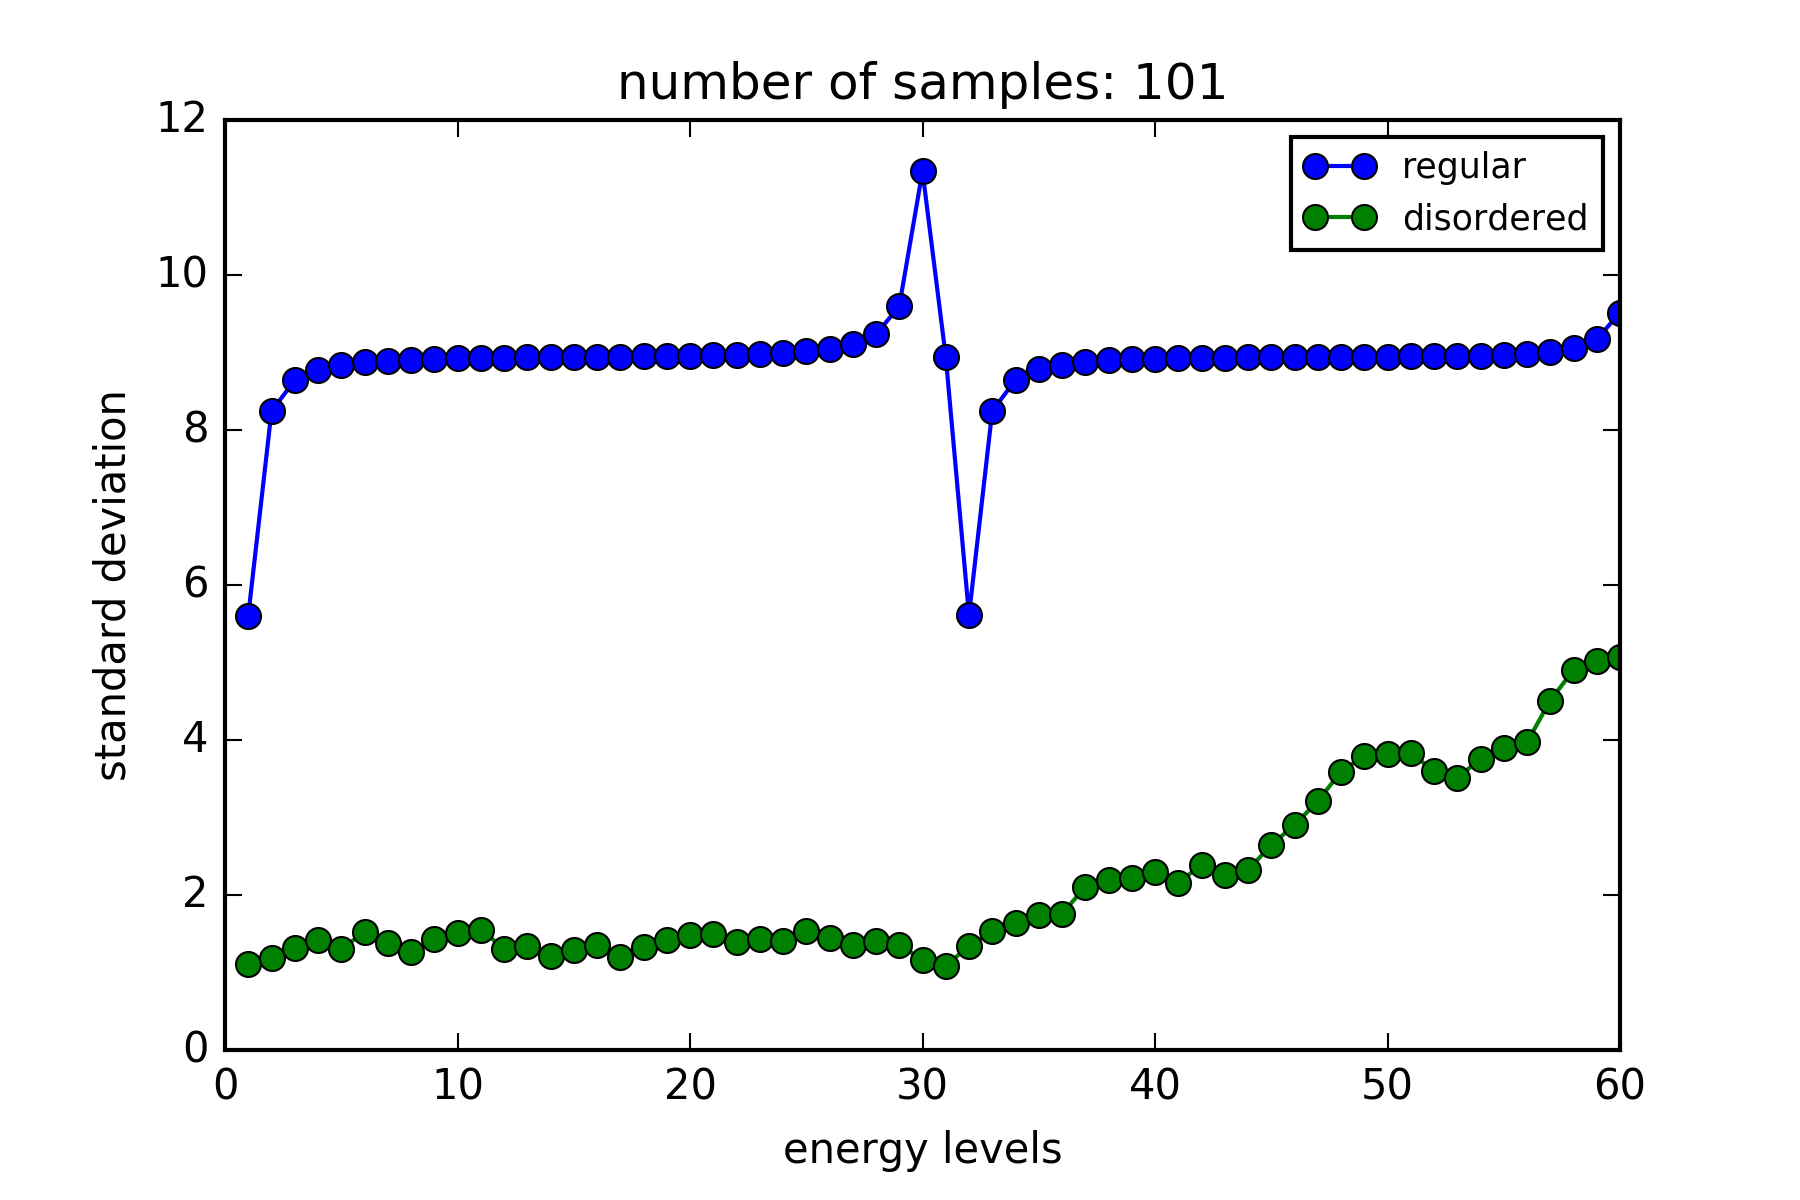
\includegraphics[width=1.1\linewidth]{standardDeviation/N_31_100a10_well0_2_p_0_5.png}
  \captionof{figure}{Localization against energy levels, comparison between Regular System and Disordered System No.6}
  \label{fig:disordered sys num 6}
\end{minipage}
\end{figure}

%a = 30 
\begin{figure}[!htbh]
\centering
\begin{minipage}{.45\textwidth}
  \centering
  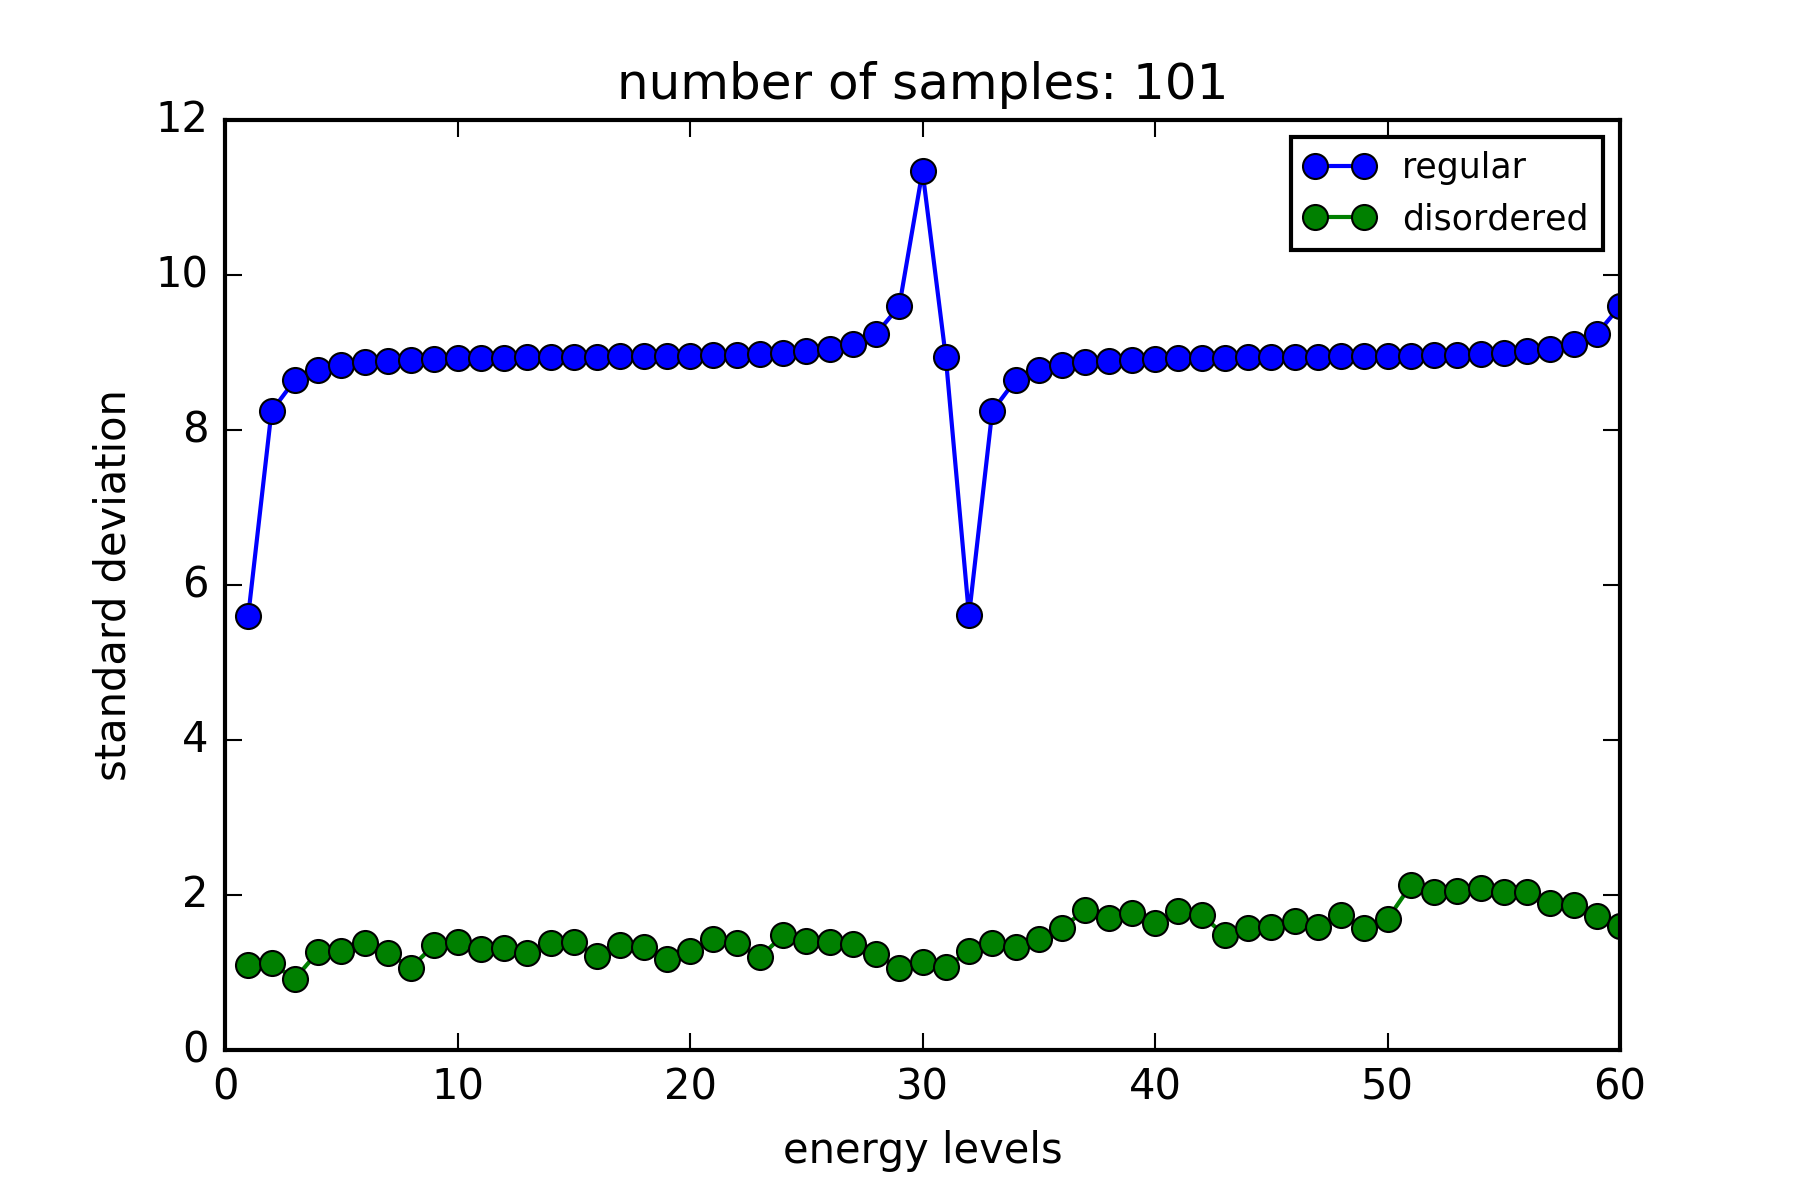
\includegraphics[width=1.1\linewidth]{standardDeviation/N_31_100a30_well0_4_p_0_5.png}
  \captionof{figure}{Localization against energy levels, comparison between Regular System and Disordered System No.7}
  \label{fig:disordered sys num 7}
\end{minipage}\qquad
\begin{minipage}{.45\textwidth}
  \centering
  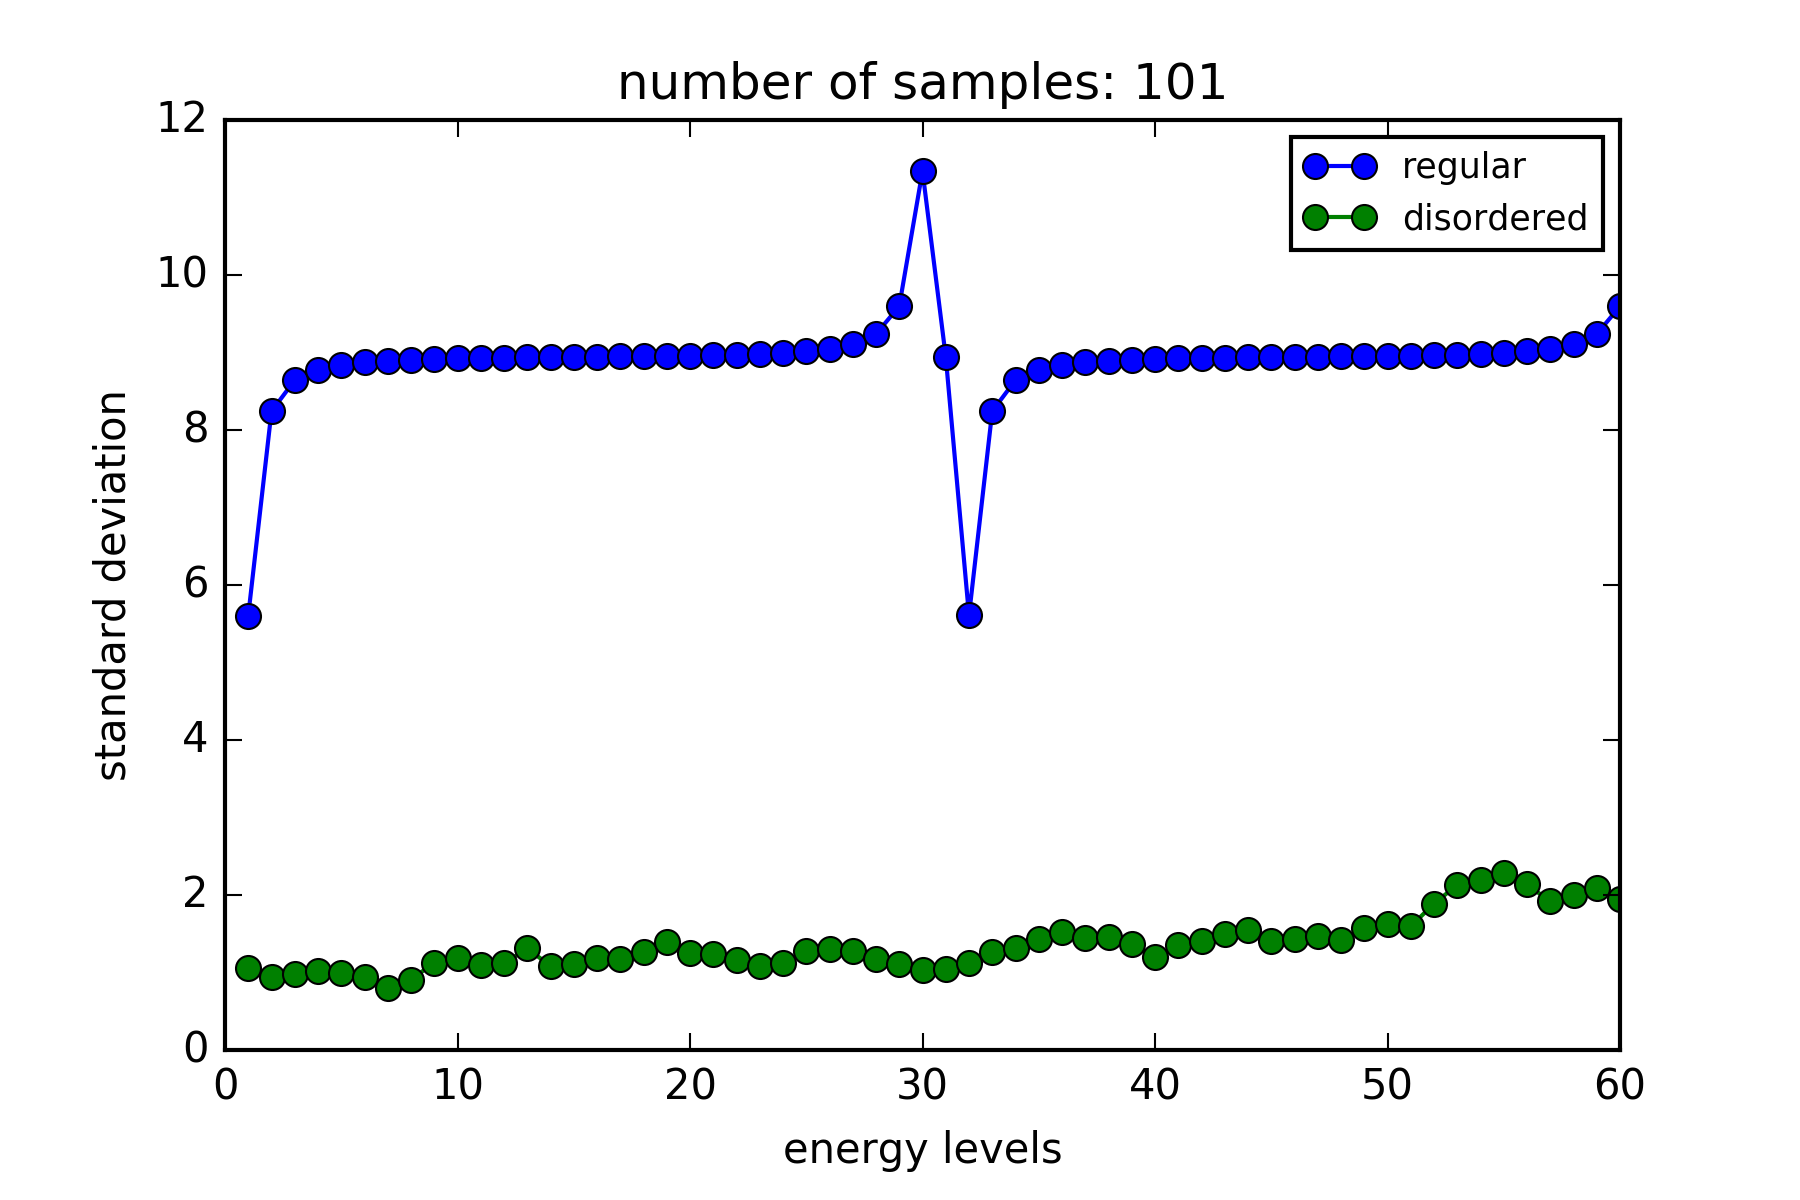
\includegraphics[width=1.1\linewidth]{standardDeviation/N_31_100a30_well0_2_p_0_5.png}
  \captionof{figure}{Localization against energy levels, comparison between Regular System and Disordered System No.8}
  \label{fig:disordered sys num 8}
\end{minipage}
\end{figure}

%end figure



\newpage
\section{Localization of normal modes in harmonic chain model}
\subsection{Randomness in atoms' mass}
The following graphs are normal modes for model 3a in which we introduce randomness to the atom mass at each site by the way we mentioned in Chapter \ref{Ch:Background} model 3b. We retain the same notation as in that section, namely $\{M_1,M_2\}$, and $\{P(M_1),P(M_2)\}$.
For better comparison, probability density function is computed by rescaling to the interval $[0,1]$ and then squaring displacements in the normal mode followed by normalization such that the total area under is 1.
The eigenvalue for each normal mode corresponds to the frequency of that normal mode.
The following are figures plotted when $\{M_1,M_2\} = \{1,2\}$ at different normal modes. Note the normal mode is on the left and the corresponding probability density function is on the left.

%0.5,{1,2} ,26th, 76th, N = 103  
\begin{figure}[!htbh]
\centering
\begin{minipage}{.45\textwidth}
  \centering
  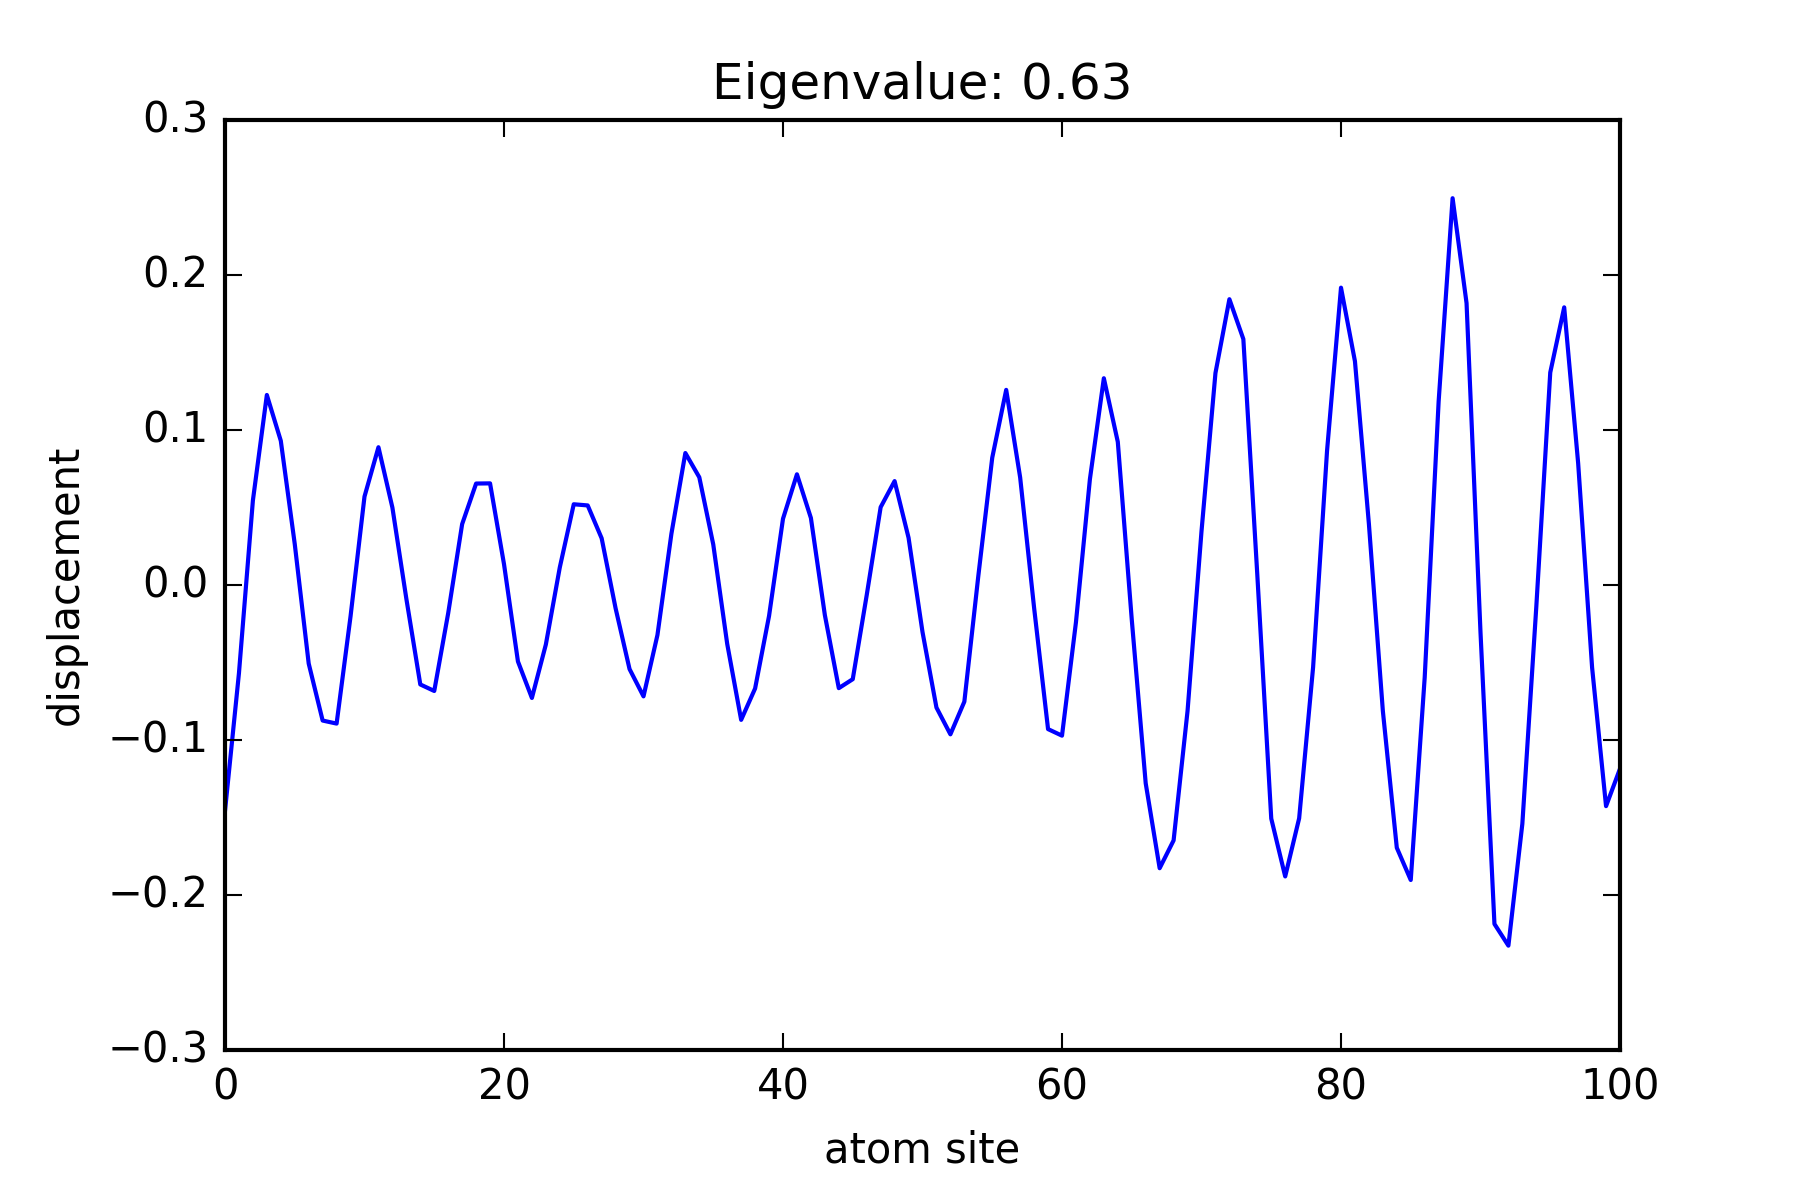
\includegraphics[width=1.1\linewidth]{Harmonic_mass_ratio/normal_Prob_0_5N_103m_2p_26th.png}
  \captionof{figure}{ $N = 103 $, $\{P(M_1),P(M_2) \}= \{0.5,0.5\} $, 26th normal mode}
  \label{fig:mass low frequency}
\end{minipage}\qquad
\begin{minipage}{.45\textwidth}
  \centering
  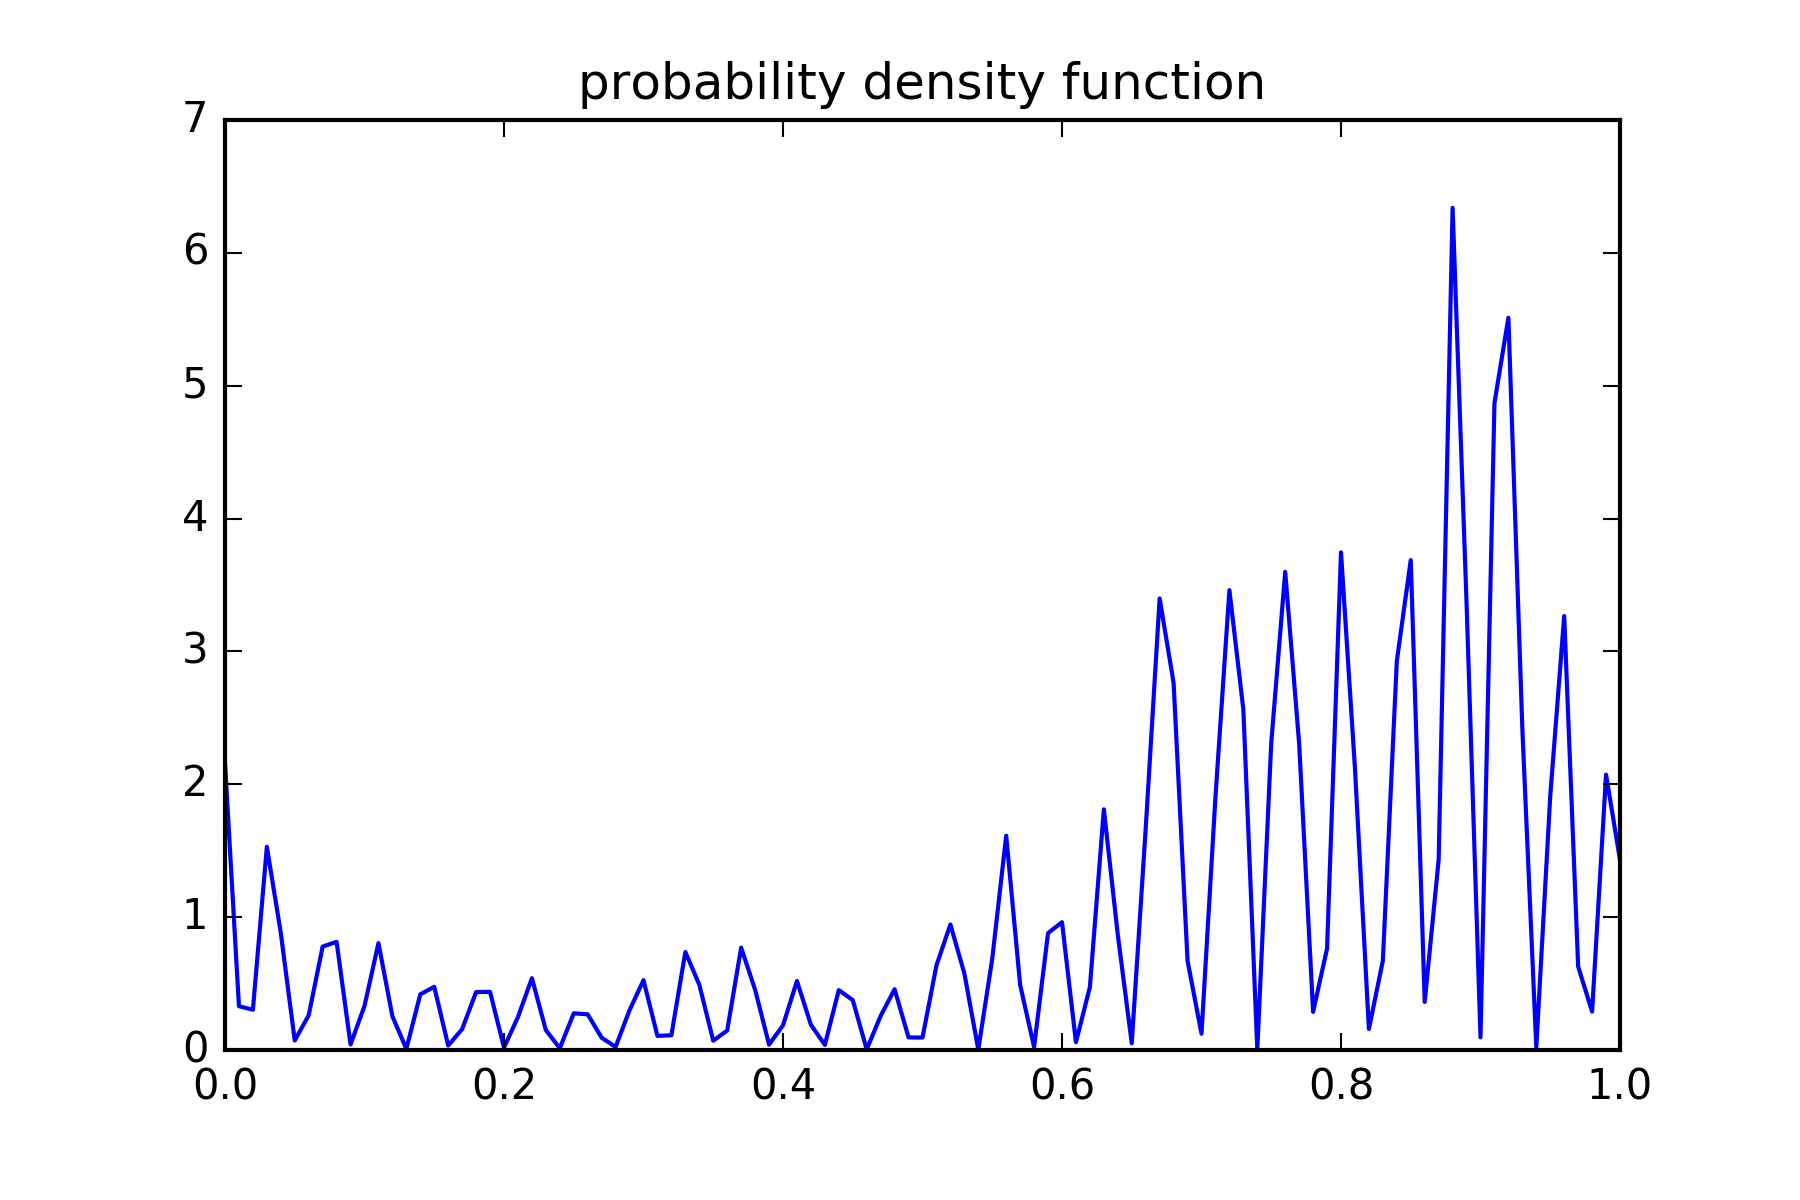
\includegraphics[width=1.1\linewidth]{Harmonic_mass_ratio/densProb_0_5N_103m_2p_26th.png}
  \captionof{figure}{ $N = 103 $, $\{P(M_1),P(M_2) \}= \{0.5,0.5\} $,26th normal mode}
  \label{fig:N103_1_2_26th_density}
\end{minipage}
\end{figure}

%0.5,{1,2} ,26th, 76th, N = 103  
\begin{figure}[!htbh]
\centering
\begin{minipage}{.45\textwidth}
  \centering
  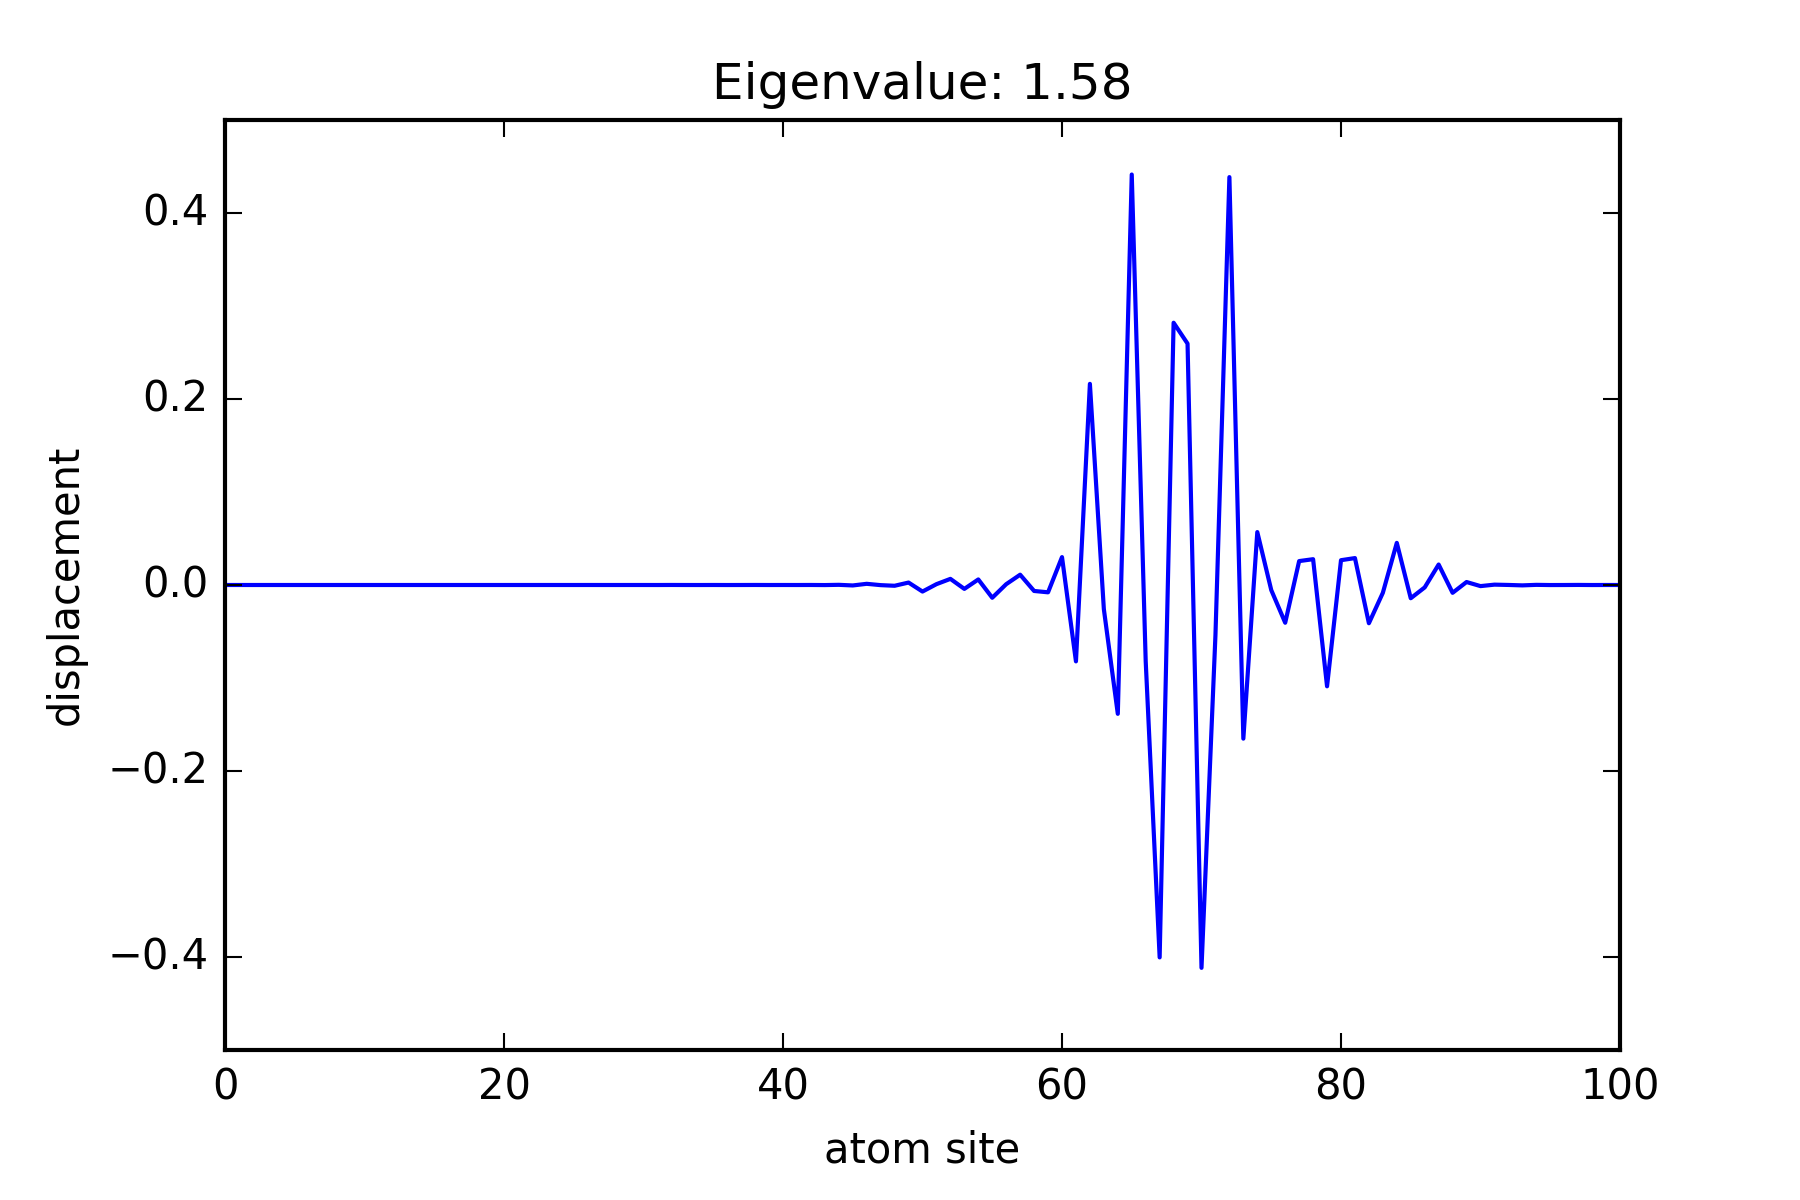
\includegraphics[width=1.1\linewidth]{Harmonic_mass_ratio/normal_Prob_0_5N_103m_2p_76th.png}
  \captionof{figure}{ $N = 103 $, $\{P(M_1),P(M_2) \}= \{0.5,0.5\} $, 76th normal mode}
  \label{fig:mass high frequency}
\end{minipage}\qquad
\begin{minipage}{.45\textwidth}
  \centering
  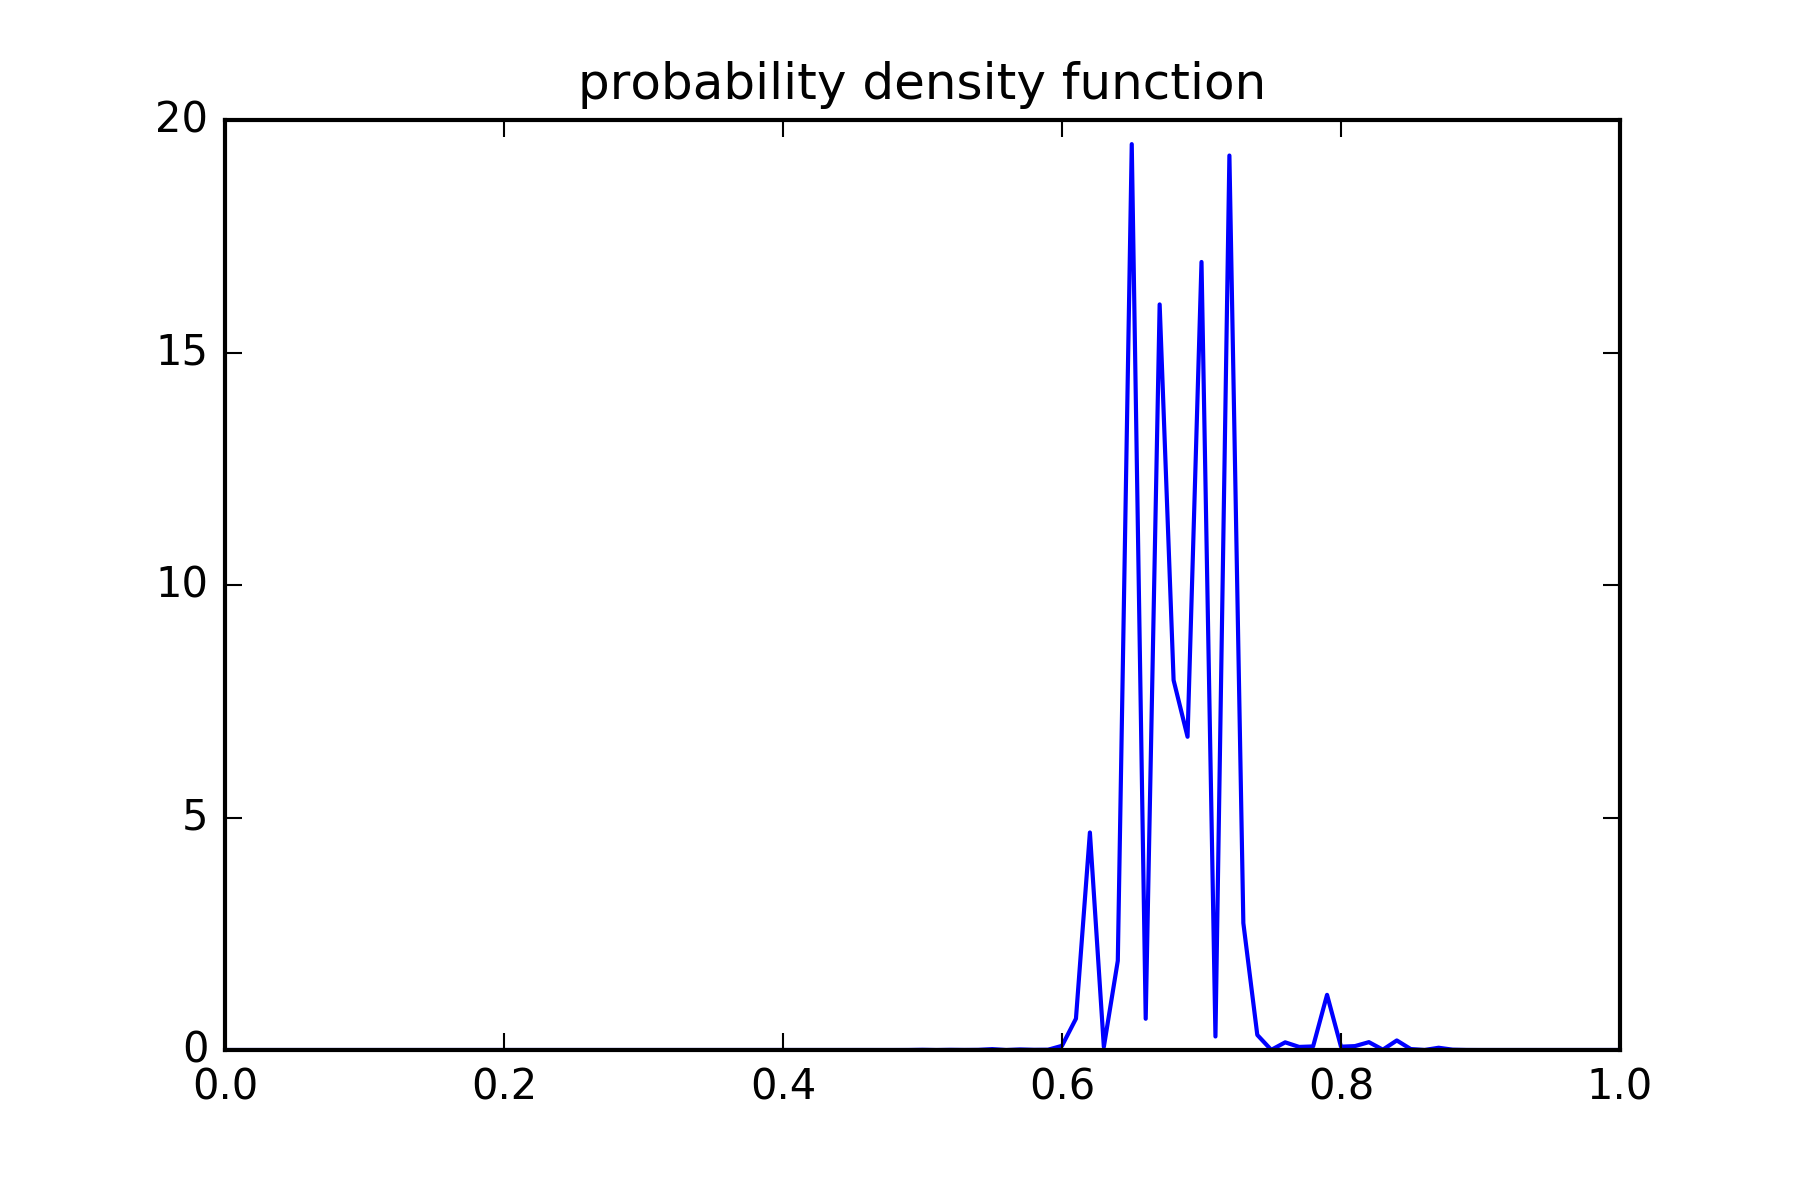
\includegraphics[width=1.1\linewidth]{Harmonic_mass_ratio/densProb_0_5N_103m_2p_76th.png}
  \captionof{figure}{ $N = 103 $, $\{P(M_1),P(M_2) \}= \{0.5,0.5\} $,76th normal mode}
  \label{fig:N103_1_2_76th_density}
\end{minipage}
\end{figure}


The following figures are for systems with different number of atoms. Only probability density functions are plotted for comparison. $\{M_1.M_2\} = \{1,2\}$.  

Since the number of normal modes is different for chains of different number of atoms. We choose a third largest frequency for comparison. That is to say for 31 atoms, we choose 28th normal mode while for 61 atoms, we choose 58th normal mode.
% N = 11, 31 ,61 , 101 

\begin{figure}[!htbh]
\centering
\begin{minipage}{.45\textwidth}
  \centering
  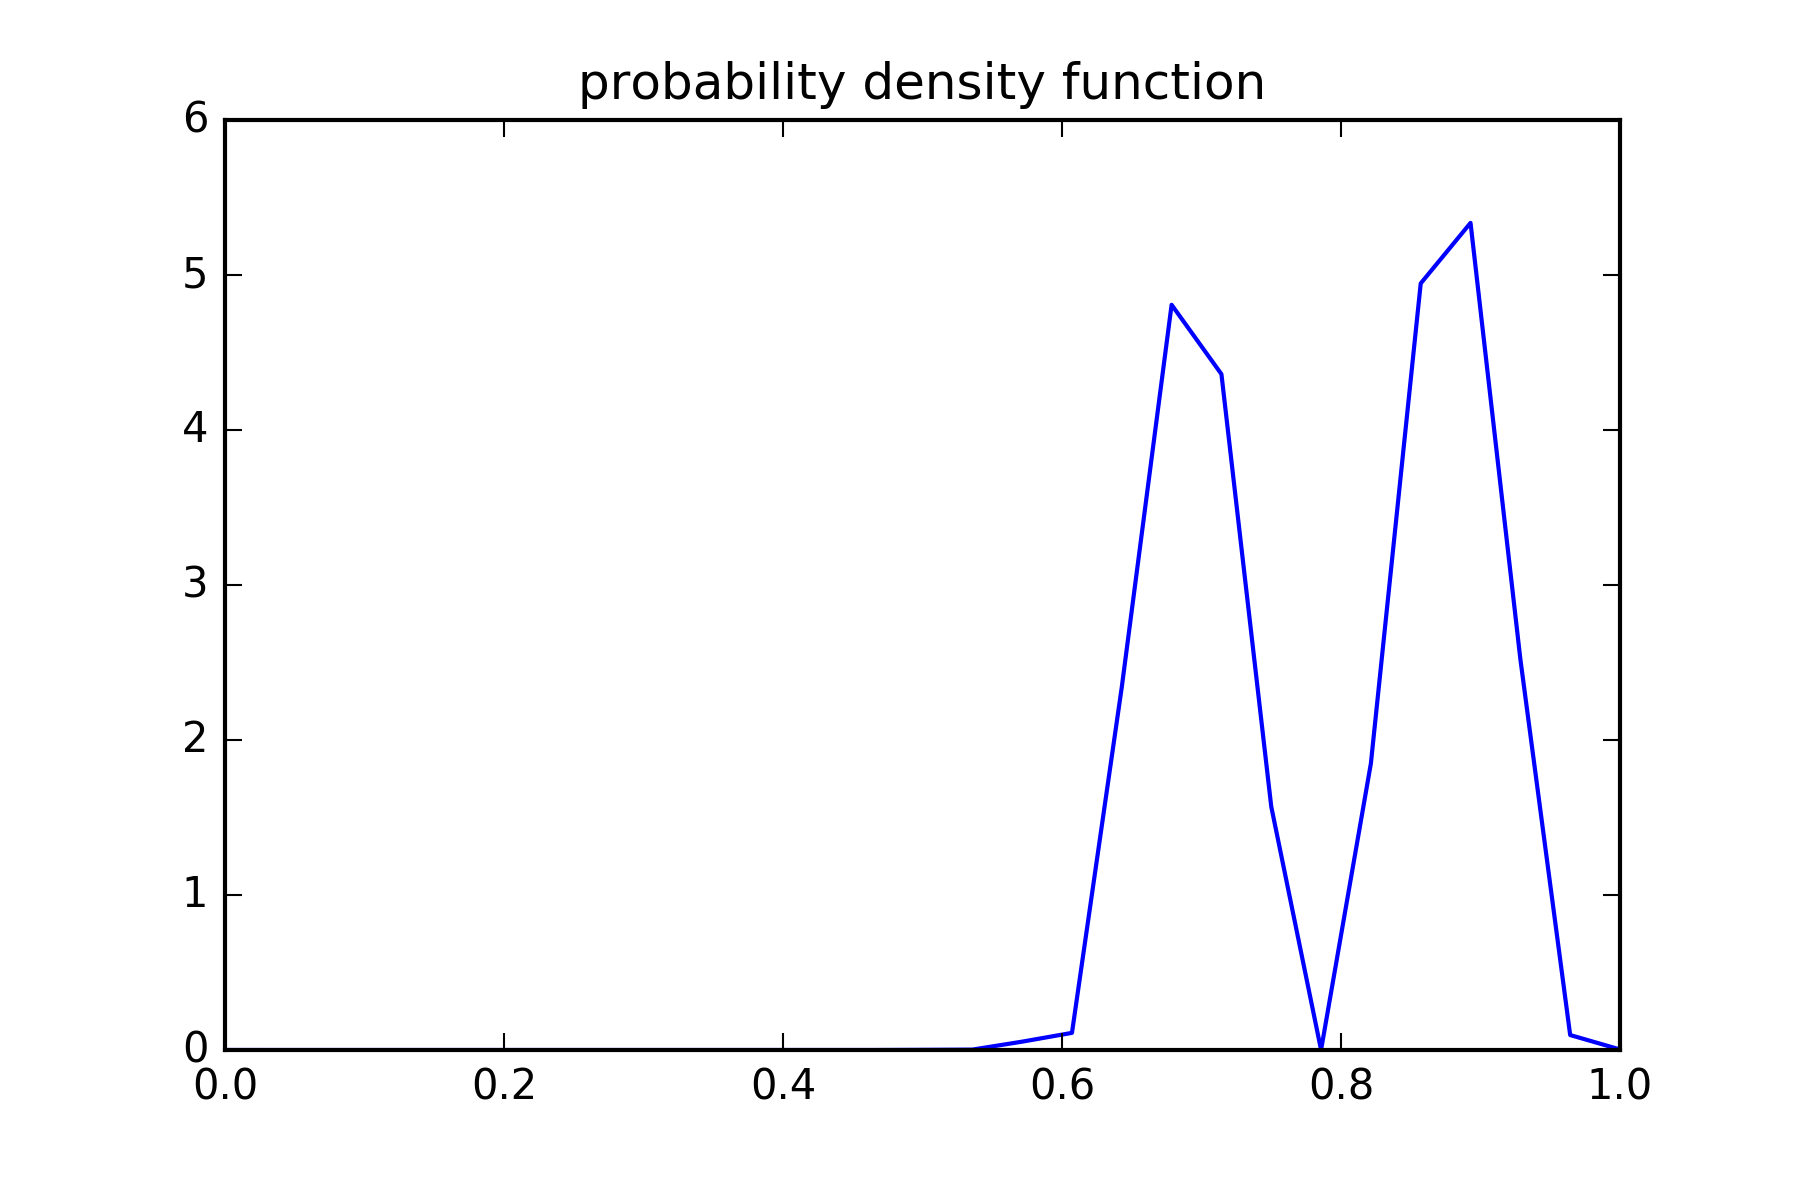
\includegraphics[width=1.1\linewidth]{Harmonic_mass_ratio/densProb_0_5N_31m_2p_28th.png}
  \captionof{figure}{ $N = 31 $, $\{P(M_1),P(M_2) \}= \{0.5,0.5\} $, 28th normal mode}
  \label{fig:mass length31 28th}
\end{minipage}\qquad
\begin{minipage}{.45\textwidth}
  \centering
  \includegraphics[width=1.1\linewidth]{Harmonic_mass_ratio/densProb_0_5N_61m_2p_58th.png}
  \captionof{figure}{ $N = 61 $, $\{P(M_1),P(M_2) \}= \{0.5,0.5\} $,58th normal mode}
  \label{fig:mass length61 58th}
\end{minipage}
\end{figure}


%101 ,201
\begin{figure}[!htbh]
\centering
\begin{minipage}{.45\textwidth}
  \centering
  \includegraphics[width=1.1\linewidth]{Harmonic_mass_ratio/densProb_0_5N_101m_2p_98th.png}
  \captionof{figure}{ $N = 101$, $\{P(M_1),P(M_2) \}= \{0.5,0.5\} $, 98th normal mode}
  \label{fig:mass length101 98th}
\end{minipage}\qquad
\begin{minipage}{.45\textwidth}
  \centering
  \includegraphics[width=1.1\linewidth]{Harmonic_mass_ratio/densProb_0_5N_201m_2p_198th.png}
  \captionof{figure}{$N = 201$, $\{P(M_1),P(M_2) \}= \{0.5,0.5\} $, 198th normal mode}
  \label{fig:mass length201 198th}
\end{minipage}
\end{figure}

\newpage
The following are figures for systems with the same number of atoms,same randomness($\{P(M_1),P(M_2) \}= \{0.5,0.5\} $), but different $\{M_1, M_2\}$. Here, we only vary $M_2$, $M_1$ is fixed to be 1. 

% N = 31, 61, 101, 201 




% M = 1.1,1.5,2.0,10.0,20.0,40.0
\begin{figure}[!htbh]
\centering
\begin{minipage}{.45\textwidth}
  \centering
  \includegraphics[width=1.1\linewidth]{Harmonic_mass_ratio/normal_Prob_0_5N_103m_1_1p_51th.png}
  \captionof{figure}{ $N = 103$, $\{M_1,M_2\} = \{1,1.1\}$, 51st normal mode}
  \label{fig:mass ratio 1.1 51st}
\end{minipage}\qquad
\begin{minipage}{.45\textwidth}
  \centering
  \includegraphics[width=1.1\linewidth]{Harmonic_mass_ratio/normal_Prob_0_5N_103m_1_5p_51th.png}
  \captionof{figure}{$N = 103$, $\{M_1,M_2\} = \{1,1.5\}$, 51st normal mode}
  \label{fig:mass ratio 1.5 51st}
\end{minipage}
\end{figure}

%2,10
\begin{figure}[!htbh]
\centering
\begin{minipage}{.45\textwidth}
  \centering
  \includegraphics[width=1.1\linewidth]{Harmonic_mass_ratio/normal_Prob_0_5N_103m_2_0p_51th.png}
  \captionof{figure}{ $N = 103$, $\{M_1,M_2\} = \{1,2\}$, 51st normal mode}
  \label{fig:mass ratio 2.0 51st}
\end{minipage}\qquad
\begin{minipage}{.45\textwidth}
  \centering
  \includegraphics[width=1.1\linewidth]{Harmonic_mass_ratio/normal_Prob_0_5N_103m_10_0p_51th.png}
  \captionof{figure}{$N = 103$, $\{M_1,M_2\} = \{1,10\}$, 51st normal mode}
  \label{fig:mass ratio 10.0 51st}
\end{minipage}
\end{figure}

%20, 40 

\begin{figure}[!htbh]
\centering
\begin{minipage}{.45\textwidth}
  \centering
  \includegraphics[width=1.1\linewidth]{Harmonic_mass_ratio/normal_Prob_0_5N_103m_20_0p_51th.png}
  \captionof{figure}{ $N = 51$, $\{M_1,M_2\} = \{1,20\}$, 51st normal mode}
  \label{fig:mass ratio 20.0 51st}
\end{minipage}\qquad
\begin{minipage}{.45\textwidth}
  \centering
  \includegraphics[width=1.1\linewidth]{Harmonic_mass_ratio/normal_Prob_0_5N_103m_40_0p_51th.png}
  \captionof{figure}{$N = 51$, $\{M_1,M_2\} = \{1,40\}$, 41th normal mode}
  \label{fig:mass ratio 40.0 51st}
\end{minipage}
\end{figure}

\newpage
The following are figures for systems with the same number of atoms,same $\{M_1, M_2\}$, but different $\{P(M_1), P(M_2)\}$. Here, we compare 2 different probabilities, namely $\{0.1, 0.9\}$ and $\{0.5, 0.5\}$. 

%26th
\begin{figure}[!htbh]
\centering
\begin{minipage}{.45\textwidth}
  \centering
  \includegraphics[width=1.1\linewidth]{Harmonic_mass_ratio/normal_Prob_0_1N_103m_2p_26th.png}
  \captionof{figure}{ $N = 103$, $\{P(M_1), P(M_2)\}= \{0.1,0.9\}$ ,$\{M_1,M_2\} = \{1,2\}$, 26th normal mode}
  \label{fig:mass prob 0.1 26th}
\end{minipage}\qquad
\begin{minipage}{.45\textwidth}
  \centering
  \includegraphics[width=1.1\linewidth]{Harmonic_mass_ratio/normal_Prob_0_5N_103m_2p_26th.png}
  \captionof{figure}{$N = 103$,$\{P(M_1), P(M_2)\}= \{0.5,0.5\}$ , $\{M_1,M_2\} = \{1,2\}$, 26th normal mode}
  \label{fig:mass prob 0.5 26th}
\end{minipage}
\end{figure}

%51st 
\begin{figure}[!htbh]
\centering
\begin{minipage}{.45\textwidth}
  \centering
  \includegraphics[width=1.1\linewidth]{Harmonic_mass_ratio/normal_Prob_0_1N_103m_2p_51th.png}
  \captionof{figure}{ $N = 103$, $\{P(M_1), P(M_2)\}= \{0.1,0.9\}$ ,$\{M_1,M_2\} = \{1,2\}$, 51st normal mode}
  \label{fig:mass prob 0.1 51th}
\end{minipage}\qquad
\begin{minipage}{.45\textwidth}
  \centering
  \includegraphics[width=1.1\linewidth]{Harmonic_mass_ratio/normal_Prob_0_5N_103m_2p_51th.png}
  \captionof{figure}{$N = 103$,$\{P(M_1), P(M_2)\}= \{0.5,0.5\}$ , $\{M_1,M_2\} = \{1,2\}$, 51st normal mode}
  \label{fig:mass prob 0.5 51th}
\end{minipage}
\end{figure}


%76th
\begin{figure}[!htbh]
\centering
\begin{minipage}{.45\textwidth}
  \centering
  \includegraphics[width=1.1\linewidth]{Harmonic_mass_ratio/normal_Prob_0_1N_103m_2p_76th.png}
  \captionof{figure}{ $N = 103$, $\{P(M_1), P(M_2)\}= \{0.1,0.9\}$ ,$\{M_1,M_2\} = \{1,2\}$, 76th normal mode}
  \label{fig:mass prob 0.1 76th}
\end{minipage}\qquad
\begin{minipage}{.45\textwidth}
  \centering
  \includegraphics[width=1.1\linewidth]{Harmonic_mass_ratio/normal_Prob_0_5N_103m_2p_76th.png}
  \captionof{figure}{$N = 103$,$\{P(M_1), P(M_2)\}= \{0.5,0.5\}$ , $\{M_1,M_2\} = \{1,2\}$, 76th normal mode}
  \label{fig:mass prob 0.5 76th}
\end{minipage}
\end{figure}

%101st
\begin{figure}[!htbh]
\centering
\begin{minipage}{.45\textwidth}
  \centering
  \includegraphics[width=1.1\linewidth]{Harmonic_mass_ratio/normal_Prob_0_1N_103m_2p_101th.png}
  \captionof{figure}{ $N = 103$, $\{P(M_1), P(M_2)\}= \{0.1,0.9\}$ ,$\{M_1,M_2\} = \{1,2\}$, 101st normal mode}
  \label{fig:mass prob 0.1 101th}
\end{minipage}\qquad
\begin{minipage}{.45\textwidth}
  \centering
  \includegraphics[width=1.1\linewidth]{Harmonic_mass_ratio/normal_Prob_0_5N_103m_2p_101th.png}
  \captionof{figure}{$N = 103$,$\{P(M_1), P(M_2)\}= \{0.5,0.5\}$ , $\{M_1,M_2\} = \{1,2\}$, 101st normal mode}
  \label{fig:mass prob 0.5 101th}
\end{minipage}
\end{figure}


\newpage
\subsection{Randomness in harmonic strings' elastic constant}
The following graphs are normal modes for model 3b in which we introduce randomness to the harmonic strings' elastic constant by the way we mentioned in section \ref{Ch:Background} model 3c. We retain the same notation as in that section, namely $\{K_1,K_2\}$, and $\{P(K_1),P(K_2)\}$. 
For better comparison between chains of different number of atoms, probability density function is sometimes computed by rescaling to the interval $[0,1]$ and then squaring displacements in the normal mode followed by normalization such that the total area under is 1.


The following are figures plotted when $\{K_1,K_2\} = \{1,2\}$ at different normal modes. Note the normal mode is on the left and the corresponding probability density function is on the left.

%spring constant ratio: 0.5,{1,2} ,26th, 76th, N = 103  
\begin{figure}[!htbh]
\centering
\begin{minipage}{.45\textwidth}
  \centering
  \includegraphics[width=1.1\linewidth]{Harmonic_spring_ratio/spr_N_103sp_2p_0_526th.png}
  \captionof{figure}{ $N = 103 $, $\{P(M_1),P(M_2) \}= \{0.5,0.5\} $, 26th normal mode}
  \label{fig:spring normal mode low frequency}
\end{minipage}\qquad
\begin{minipage}{.45\textwidth}
  \centering
  \includegraphics[width=1.1\linewidth]{Harmonic_spring_ratio/densProb_0_5N_103m_2p_26th.png}
  \captionof{figure}{ $N = 103 $, $\{P(M_1),P(M_2) \}= \{0.5,0.5\} $,26th normal mode}
  \label{fig:spring prob density low frequency}
\end{minipage}
\end{figure}

%56th 
\begin{figure}[!htbh]
\centering
\begin{minipage}{.45\textwidth}
  \centering
  \includegraphics[width=1.1\linewidth]{Harmonic_spring_ratio/spr_N_103sp_2p_0_551th.png}
  \captionof{figure}{ $N = 103 $, $\{P(M_1),P(M_2) \}= \{0.5,0.5\} $, 51st normal mode}
  \label{fig:spring normal mode mid range frequency}
\end{minipage}\qquad
\begin{minipage}{.45\textwidth}
  \centering
  \includegraphics[width=1.1\linewidth]{Harmonic_spring_ratio/densProb_0_5N_103m_2p_51th.png}
  \captionof{figure}{ $N = 103 $, $\{P(M_1),P(M_2) \}= \{0.5,0.5\} $,51st normal mode}
  \label{fig:spring prob density mid range frequency}
\end{minipage}
\end{figure}

%76th 
\begin{figure}[!htbh]
\centering
\begin{minipage}{.45\textwidth}
  \centering
  \includegraphics[width=1.1\linewidth]{Harmonic_spring_ratio/spr_N_103sp_2p_0_576th.png}
  \captionof{figure}{ $N = 103 $, $\{P(M_1),P(M_2) \}= \{0.5,0.5\} $, 76th normal mode}
  \label{fig:spring normal mode high frequency}
\end{minipage}\qquad
\begin{minipage}{.45\textwidth}
  \centering
  \includegraphics[width=1.1\linewidth]{Harmonic_spring_ratio/densProb_0_5N_103m_2p_76th.png}
  \captionof{figure}{ $N = 103 $, $\{P(M_1),P(M_2) \}= \{0.5,0.5\} $,76th normal mode}
  \label{fig:spring prob density high frequency}
\end{minipage}
\end{figure}


%2 
\newpage
The following figures are for systems with different number of atoms. Only probability density functions are plotted for comparison. 

%spring N = 31, 61 
\begin{figure}[!htbh]
\centering
\begin{minipage}{.45\textwidth}
  \centering
  \includegraphics[width=1.1\linewidth]{Harmonic_spring_ratio/densProb_0_5N_31m_2p_28th.png}
  \captionof{figure}{ $N = 31 $, $\{P(K_1),P(K_2) \}= \{0.5,0.5\} $, 28th normal mode}
  \label{fig:spring_N_31m_2_28th}
\end{minipage}\qquad
\begin{minipage}{.45\textwidth}
  \centering
  \includegraphics[width=1.1\linewidth]{Harmonic_spring_ratio/densProb_0_5N_61m_2p_58th.png}
  \captionof{figure}{ $N = 61 $, $\{P(K_1),P(K_2) \}= \{0.5,0.5\} $,58th normal mode}
  \label{fig:spring_N_61m_2_58th}
\end{minipage}
\end{figure}


%101 ,201
\begin{figure}[!htbh]
\centering
\begin{minipage}{.45\textwidth}
  \centering
  \includegraphics[width=1.1\linewidth]{Harmonic_spring_ratio/densProb_0_5N_101m_2p_98th.png}
  \captionof{figure}{ $N = 101$, $\{P(K_1),P(K_2) \}= \{0.5,0.5\} $, 98th normal mode}
  \label{fig:spring_N_101m_2_98th}
\end{minipage}\qquad
\begin{minipage}{.45\textwidth}
  \centering
  \includegraphics[width=1.1\linewidth]{Harmonic_spring_ratio/densProb_0_5N_201m_2p_198th.png}
  \captionof{figure}{$N = 201$, $\{P(K_1),P(K_2) \}= \{0.5,0.5\} $, 198th normal mode}
  \label{fig:spring_N_201m_2_198th}
\end{minipage}
\end{figure}


%3
\newpage
The following are figures for systems with the same number of atoms,same randomness($\{P(K_1),P(K_2) \}= \{0.5,0.5\} $), but different $\{K_1, K_2\}$. Here, we only vary $K_2$. $K_1$ is fixed to be 1. 



% K_2 = 1.1,1.5,2.0,10.0,20.0,40.0
\begin{figure}[!htbh]
\centering
\begin{minipage}{.45\textwidth}
  \centering
  \includegraphics[width=1.1\linewidth]{Harmonic_spring_ratio/spr_N_103sp_1_1p_0_576th.png}
  \captionof{figure}{ $N = 103$, $\{K_1,K_2\} = \{1,1.1\}$, 76th normal mode}
  \label{fig:spring_N_103m_1.1_p_0_5_76th}
\end{minipage}\qquad
\begin{minipage}{.45\textwidth}
  \centering
  \includegraphics[width=1.1\linewidth]{Harmonic_spring_ratio/spr_N_103sp_1_5p_0_576th.png}
  \captionof{figure}{$N = 103$, $\{K_1,K_2\} = \{1,1.5\}$, 76th normal mode}
  \label{fig:spring_N_103m_1.5_p_0_5_51st}
\end{minipage}
\end{figure}
%2, 5 
\begin{figure}[!htbh]
\centering
\begin{minipage}{.45\textwidth}
  \centering
  \includegraphics[width=1.1\linewidth]{Harmonic_spring_ratio/spr_N_103sp_2_0p_0_576th.png}
  \captionof{figure}{ $N = 103$, $\{K_1,K_2\} = \{1,2\}$, 76th normal mode}
  \label{fig:spring_N_103m_2.0_p_0_5_76th}
\end{minipage}\qquad
\begin{minipage}{.45\textwidth}
  \centering
  \includegraphics[width=1.1\linewidth]{Harmonic_spring_ratio/spr_N_103sp_5_0p_0_576th.png}
  \captionof{figure}{$N = 103$, $\{K_1,K_2\} = \{1,5\}$, 76th normal mode}
  \label{fig:spring_N_103m_5.0_p_0_5_51st}
\end{minipage}
\end{figure}

%10, 20
\begin{figure}[!htbh]
\centering
\begin{minipage}{.45\textwidth}
  \centering
  \includegraphics[width=1.1\linewidth]{Harmonic_spring_ratio/spr_N_103sp_10_0p_0_576th.png}
  \captionof{figure}{ $N = 103$, $\{K_1,K_2\} = \{1,10\}$, 76th normal mode}
  \label{fig:spring_N_103m_10.0_p_0_5_76th}
\end{minipage}\qquad
\begin{minipage}{.45\textwidth}
  \centering
  \includegraphics[width=1.1\linewidth]{Harmonic_spring_ratio/spr_N_103sp_20_0p_0_576th.png}
  \captionof{figure}{$N = 103$, $\{K_1,K_2\} = \{1,20\}$, 76th normal mode}
  \label{fig:spring_N_103m_20.0_p_0_5_51st}
\end{minipage}
\end{figure}

\newpage
The following are figures for systems with the same number of atoms,same $\{K_1, K_2\}$, but different $\{P(K_1), P(K_2)\}$. Here, we compare 2 different probabilities, namely $\{0.1, 0.9\}$ and $\{0.5, 0.5\}$. 

%26th
\begin{figure}[!htbh]
\centering
\begin{minipage}{.45\textwidth}
  \centering
  \includegraphics[width=1.1\linewidth]{Harmonic_spring_ratio/prob_spr_N_103sp_2_0p_0_126th.png}
  \captionof{figure}{ $N = 103$, $\{P(K_1), P(K_2)\}= \{0.1,0.9\}$ ,$\{K_1,K_2\} = \{1,2\}$, 26th normal mode}
  \label{fig:prob_spring_N_103m_2p_0_1_26th}
\end{minipage}\qquad
\begin{minipage}{.45\textwidth}
  \centering
  \includegraphics[width=1.1\linewidth]{Harmonic_spring_ratio/prob_spr_N_103sp_2_0p_0_526th.png}
  \captionof{figure}{$N = 103$,$\{P(K_1), P(K_2)\}= \{0.5,0.5\}$ , $\{K_1,K_2\} = \{1,2\}$, 26th normal mode}
  \label{fig:prob_spring_N_103m_2p_0_5_26th}
\end{minipage}
\end{figure}

%51st
\begin{figure}[!htbh]
\centering
\begin{minipage}{.45\textwidth}
  \centering
  \includegraphics[width=1.1\linewidth]{Harmonic_spring_ratio/prob_spr_N_103sp_2_0p_0_151th.png}
  \captionof{figure}{ $N = 103$, $\{P(K_1), P(K_2)\}= \{0.1,0.9\}$ ,$\{K_1,K_2\} = \{1,2\}$, 51st normal mode}
  \label{fig:prob_spring_N_103m_2p_0_1_51st}
\end{minipage}\qquad
\begin{minipage}{.45\textwidth}
  \centering
  \includegraphics[width=1.1\linewidth]{Harmonic_spring_ratio/prob_spr_N_103sp_2_0p_0_551th.png}
  \captionof{figure}{$N = 103$,$\{P(K_1), P(K_2)\}= \{0.5,0.5\}$ , $\{K_1,K_2\} = \{1,2\}$, 51st normal mode}
  \label{fig:prob_spring_N_103m_2p_0_5_51st}
\end{minipage}
\end{figure}

%76th
\begin{figure}[!htbh]
\centering
\begin{minipage}{.45\textwidth}
  \centering
  \includegraphics[width=1.1\linewidth]{Harmonic_spring_ratio/prob_spr_N_103sp_2_0p_0_176th.png}
  \captionof{figure}{ $N = 103$, $\{P(K_1), P(K_2)\}= \{0.1,0.9\}$ ,$\{K_1,K_2\} = \{1,2\}$, 76th normal mode}
  \label{fig:prob_spring_N_103m_2p_0_1_76th}
\end{minipage}\qquad
\begin{minipage}{.45\textwidth}
  \centering
  \includegraphics[width=1.1\linewidth]{Harmonic_spring_ratio/prob_spr_N_103sp_2_0p_0_576th.png}
  \captionof{figure}{$N = 103$,$\{P(K_1), P(K_2)\}= \{0.5,0.5\}$ , $\{K_1,K_2\} = \{1,2\}$, 76th normal mode}
  \label{fig:prob_spring_N_103m_2p_0_5_76th}
\end{minipage}
\end{figure}

%101st
\begin{figure}[!htbh]
\centering
\begin{minipage}{.45\textwidth}
  \centering
  \includegraphics[width=1.1\linewidth]{Harmonic_spring_ratio/prob_spr_N_103sp_2_0p_0_1101th.png}
  \captionof{figure}{ $N = 103$, $\{P(K_1), P(K_2)\}= \{0.1,0.9\}$ ,$\{K_1,K_2\} = \{1,2\}$, 101st normal mode}
  \label{fig:prob_spring_N_103m_2p_0_1_101st}
\end{minipage}\qquad
\begin{minipage}{.45\textwidth}
  \centering
  \includegraphics[width=1.1\linewidth]{Harmonic_spring_ratio/prob_spr_N_103sp_2_0p_0_5101th.png}
  \captionof{figure}{$N = 103$,$\{P(K_1), P(K_2)\}= \{0.5,0.5\}$ , $\{K_1,K_2\} = \{1,2\}$, 101st normal mode}
  \label{fig:prob_spring_N_103m_2p_0_5_101st}
\end{minipage}
\end{figure}


\endinput